%%%%%%%%%%%%%%%%%%%%%%%%%%%%%%%%%%%%%%%%%
% Short Sectioned Assignment LaTeX Template Version 1.0 (5/5/12)
% This template has been downloaded from: http://www.LaTeXTemplates.com
% Original author:  Frits Wenneker (http://www.howtotex.com)
% License: CC BY-NC-SA 3.0 (http://creativecommons.org/licenses/by-nc-sa/3.0/)
%%%%%%%%%%%%%%%%%%%%%%%%%%%%%%%%%%%%%%%%%

% \documentclass[paper=a4, fontsize=11pt]{scrartcl} % A4 paper and 11pt font size
\documentclass[11pt, a4paper]{book}
\usepackage[T1]{fontenc} % Use 8-bit encoding that has 256 glyphs
\usepackage[utf8]{inputenc}
\usepackage{fourier} % Use the Adobe Utopia font for the document - comment this line to return to the LaTeX default
\usepackage{listings} % para insertar código con formato similar al editor
\usepackage[spanish, es-tabla]{babel} % Selecciona el español para palabras introducidas automáticamente, p.ej. "septiembre" en la fecha y especifica que se use la palabra Tabla en vez de Cuadro
\usepackage{url} % ,href} %para incluir URLs e hipervínculos dentro del texto (aunque hay que instalar href)
\usepackage{graphics,graphicx, float} %para incluir imágenes y colocarlas
\usepackage[gen]{eurosym} %para incluir el símbolo del euro
\usepackage{cite} %para incluir citas del archivo <nombre>.bib
\usepackage{enumerate}
\usepackage{hyperref}
\usepackage{graphicx}
\usepackage{tabularx}
\usepackage{booktabs}
\usepackage{amsmath}
\usepackage{amsfonts,amssymb}
\usepackage[center]{caption}

\usepackage[table,xcdraw]{xcolor}
\hypersetup{
	colorlinks=true,	% false: boxed links; true: colored links
	linkcolor=black,	% color of internal links
	urlcolor=cyan,		% color of external links
	citecolor=blue
}
\renewcommand{\familydefault}{\sfdefault}
\usepackage{fancyhdr} % Custom headers and footers
\pagestyle{fancyplain} % Makes all pages in the document conform to the custom headers and footers
\fancyhead[L]{} % Empty left header
\fancyhead[C]{} % Empty center header
\fancyhead[R]{Sergio García Cabrera} % My name
\fancyfoot[L]{} % Empty left footer
\fancyfoot[C]{} % Empty center footer
\fancyfoot[R]{\thepage} % Page numbering for right footer
%\renewcommand{\headrulewidth}{0pt} % Remove header underlines
\renewcommand{\footrulewidth}{0pt} % Remove footer underlines
\definecolor{backcolour}{rgb}{0.95,0.95,0.92}
\lstset{
	backgroundcolor=\color{backcolour},
	basicstyle=\ttfamily,
	columns=fullflexible,
	frame=single,
	breaklines=true,
	escapeinside={\%*}{*)},
	aboveskip=\bigskipamount,
	belowskip=\bigskipamount,
	showstringspaces=false,
	tabsize=2
}
\setlength{\headheight}{13.6pt} % Customize the height of the header

\usepackage{titlesec, blindtext, color}
\definecolor{gray75}{gray}{0.75}
\newcommand{\hsp}{\hspace{20pt}}
\titleformat{\chapter}[hang]{\Huge\bfseries}{\thechapter\hsp\textcolor{gray75}{|}\hsp}{0pt}{\Huge\bfseries}
\setcounter{secnumdepth}{4}
\usepackage[Lenny]{fncychap}
\graphicspath{{./pictures/}}
\newcommand{\shellcmd}[1]{\\\indent\indent\texttt{\footnotesize\# #1}\\}

\begin{document}

	% Plantilla portada UGR
	\begin{titlepage}
\newlength{\centeroffset}
\setlength{\centeroffset}{-0.5\oddsidemargin}
\addtolength{\centeroffset}{0.5\evensidemargin}
\thispagestyle{empty}

\noindent\hspace*{\centeroffset}\begin{minipage}{\textwidth}

\centering

\includegraphics[width=0.9\textwidth]{logos/logo_ugr.jpg}\\[1.4cm]

\textsc{ \Large TRABAJO FIN DE GRADO\\[0.2cm]}
\textsc{ GRADO EN INGENIERIA INFORMATICA}\\[1cm]

{\Huge\bfseries Título \\}
\noindent\rule[-1ex]{\textwidth}{3pt}\\[3.5ex]
{\large\bfseries Subtítulo }
\end{minipage}

\vspace{2.5cm}
\noindent\hspace*{\centeroffset}
\begin{minipage}{\textwidth}
\centering

\textbf{Autor}\\ {Estudiante}\\[2.5ex]
\textbf{Director}\\ {Tutor(a)(es)}\\[2cm]

\includegraphics[width=0.3\textwidth]{logos/etsiit_logo.png}\\[0.1cm]
\textsc{Escuela Técnica Superior de Ingenierías Informática y de Telecomunicación}\\
\textsc{---}\\
Granada, Junio de 201x
\end{minipage}
\end{titlepage}


	% Plantilla prefacio UGR
	\thispagestyle{empty}

\begin{center}
{\large\bfseries Introducción al Fuzzing, uso y estrategias de Fuzzing
para encontrar vulnerabilidades en dispositivos IoT}\\
\end{center}
\begin{center}
Sergio García Cabrera\\
\end{center}

%\vspace{0.7cm}

\vspace{0.5cm}
\noindent{\textbf{Palabras clave}: \textit{Fuzzing, IoT, Emulación, Vulnerabilidad, Sistemas empotrados,
,Black-box fuzzing, AFL++, QEMU, Open Source.}
\vspace{0.7cm}

\noindent{\textbf{Resumen}\\
Dado el creciente incremento de dispositivos conectados a internet a nuestro alrededor y la cada vez más 
sensible información que estos manejan, es una necesidad innegable el invertir una mayor cantidad de
recursos en la protección y evaluación de la seguridad de estos productos. Por desgracia, la seguridad de 
estos es en numerosas ocasiones dejada de lado debido a diferentes motivos como las 
grandes restricciones de rendimiento y de entorno normalmente asociadas a dichos dispositivos o los intentos por parte
de los fabricantes de abaratar costes de producción en productos low-cost del internet de las cosas. \\

Esta misma tendencia se puede observar respecto a la técnica del fuzzing. Aunque el fuzzing se ha consolidado 
en los últimos años como una técnica estándar en la industria del 
software gracias a su gran capacidad para encontrar fallos y vulnerabilidades, el fuzzing orientado a 
dispositivos IoT y por ende, dispositivos empotrados es un campo de investigación considerablemente 
reciente en el que aún se están dando los primeros pasos. Sumando a las causas descritas anteriormente, 
esto se debe a que aplicar técnicas de fuzzing a este tipo de dispositivos supone nuevos retos como la 
dificultad de obtener feedback sobre la ejecución de los bloques básicos de código sin disponer del código
fuente original.

En este proyecto se investigarán y aplicarán diversos enfoques y técnicas estado del arte con el fin de 
conocer el estado actual de esta novedosa rama del fuzzing orientado a dispositivos IoT.
\cleardoublepage

\begin{center}
	{\large\bfseries Introduction to Fuzzing, use cases and strategies 
	to find vulnerabilities in IoT devices}\\
\end{center}
\begin{center}
	Sergio García Cabrera\\
\end{center}
\vspace{0.5cm}
\noindent{\textbf{Keywords}: \textit{Fuzzing, IoT, Emulation, Vulnerability, Embedded systems,
,Black-box fuzzing, AFL++, QEMU, Open Source.}
\vspace{0.7cm}

\noindent{\textbf{Abstract}\\
Given the ever-increasing rise in the number of devices connected to the internet around us and the fact 
that nowadays these are made to handle more sensible information, it is clear that it has become a 
necessity to invest more time and resources in the protection and evaluation of the security of these 
products. Unfortunately, the security measures found on these are often left aside due to reasons such as 
the performance and environment constraints commonly associated with these kinds of devices or manufacturers
trying to reduce production costs of low-cost IoT devices.\\

The same trend can be observed regarding fuzzing. Even though fuzzing has consolidated as an industry 
standard thanks to its great success finding bugs and vulnerabilities in code, IoT oriented 
fuzzing and, by extension, embedded oriented fuzzing is a research field that is not nearly as mature.
Adding up to the aforementioned issues, applying fuzzing techniques to this kind of devices comes with new 
challenges such as the difficulty to get feedback about execution of basic code blocks due to the lack of 
original source code.

In this thesis, different state-of-the-art techniques and approaches will be discussed and applied in order
to learn about the current state of such a novel research field that is IoT oriented fuzzing.
\cleardoublepage

\thispagestyle{empty}

\noindent\rule[-1ex]{\textwidth}{2pt}\\[4.5ex]

D. \textbf{Gustavo Romero López}, Profesor(a) del ...

\vspace{0.5cm}

\textbf{Informo:}

\vspace{0.5cm}

Que el presente trabajo, titulado \textit{\textbf{Introducción al Fuzzing, uso y estrategias de Fuzzing
para encontrar vulnerabilidades en dispositivos IoT}},
ha sido realizado bajo mi supervisión por \textbf{Sergio García Cabrera}, y autorizo la defensa de dicho trabajo ante el tribunal
que corresponda.

\vspace{0.5cm}

Y para que conste, expiden y firman el presente informe en Granada a Junio de 2022.

\vspace{1cm}

\textbf{El/la director(a)/es: }

\vspace{5cm}

\noindent \textbf{Gustavo Romero López}

\chapter*{Agradecimientos}
Quiero agradecer a mi familia por haberme acompañado y apoyado durante todo este viaje, especialmente
en esos momentos en los que creía que no sería capaz de seguir adelante. A mis amigos y mi pareja por 
ayudarme cuando tanto necesitaba desconectar y despejarme y por último a mi tutor, Gustavo Romero López
por orientarme pacientemente cuando ni siquiera sabía cómo enfocar el TFG.





	% Índice de contenidos
	\newpage
	\tableofcontents

	% Índice de imágenes y tablas
	\newpage
	\listoffigures

	% Si hay suficientes se incluirá dicho índice
	\listoftables 
	\newpage

	% Introducción 
	\chapter{Introducción}
\label{introduccion}

\section{Motivación}
En la actualidad, podemos fácilmente apreciar cómo los fabricantes de productos de todo tipo de
ámbitos como pueden ser la medicina, la industria, la seguridad o incluso el hogar, apuestan cada vez 
más por desarrollar nuevas iteraciones de estos productos con funcionalidades comúnmente agrupadas bajo el 
adjetivo de inteligentes o ''smart''. Este nuevo paradigma de dispositivos inteligentes capaces de 
comunicarse entre sí y trabajar de forma coordinada conocido como el ''Internet de las Cosas'' o IoT por 
sus siglas en Inglés ha experimentado un crecimiento descontrolado durante la última década debido 
principalmente a los avances realizados en campos como las telecomunicaciones o el diseño de procesadores y
SoCs con una mayor potencia y menor consumo. Tal es el crecimiento que actualmente se espera que la industria del
IoT pueda alcanzar un valor económico potencial de entre 5.5 y 12.6 miles de millones de dólares para
2030 \cite{McKinsey}.
\bigskip
Dispositivos no tan novedosos como cámaras IP o routers, al igual que otros más 
propios de la última década como asistentes de voz, Smart TVs o wearables son todos ejemplos 
de dispositivos IoT que han conseguido ser una parte esencial de nuestro día a día facilitándonos
multitud de tareas. Aunque no es secreto que este tipo de dispositivos suelen basar su funcionalidad en 
la recopilación y comunicación de información que puede llegar a ser considerada sensible, es una realidad 
que los fabricantes de dichos dispositivos no están realizando una inversión suficiente en su seguridad y 
la de los datos que manejan. Un claro ejemplo de ello es el hecho de que en Europa, casi la mitad 
de dispositivos del fabricante TP-Link utiliza credenciales por defecto \cite{Deepak}, sin forzar al usuario 
a cambiarlas o incluso el gran número de estos que son puestos a la venta a día de hoy utilizando software 
considerablemente desactualizado y vulnerable como pueden ser versiones del kernel de linux publicadas hace cerca de 
diez años y ya consideradas ''End Of Life''. Problemas como los mencionados dan lugar a grandes brechas de
seguridad, que explotadas por un atacante pueden tener consecuencias desastrosas. Ejemplo de ello es 
Mirai\cite{mirai}, un malware que identificaba dispositivos IoT como routers o cámaras IP que usaran credenciales 
por defecto conocidas para infectarlos y crear una botnet que permitiera realizar ataques DDoS a gran escala.\\

Existen diversas causas que nos pueden ayudar a comprender el estado actual de la seguridad en el campo del IoT.
En primer lugar, es necesario tener en cuenta que estamos ante una industria relativamente 
joven, en claro auge y con un gran interés para todo tipo de compañías que quieren introducirse en ella diseñando 
nuevos productos pero muchas de ellas con la dificultad añadida de carecer de experiencia previa en el sector.
Esta falta de experiencia puede llevar a tomar decisiones como el realizar lanzamientos apresurados en los que la seguridad del producto no haya 
sido evaluada adecuadamente o el buscar reducir costes obviando aspectos de seguridad que puedan afectar a 
la tríada CIA (Confidentiality, Integrity, Availability) en productos de gamas low-cost donde el margen de beneficio 
es más estrecho. Respecto a vulnerabilidades software, un factor clave a tener en cuenta es la dificultad en muchos de estos 
dispositivos para que el usuario final actualice su firmware. Los altos niveles de complejidad y el gran número de dependencias del software
que es desarrollado hoy en día convierte la pregunta de \textit{¿Es este producto software vulnerable?} en algo más parecido a 
\textit{¿Cuánto tiempo tardará su seguridad en verse comprometida?} Esta realidad ejemplifica la necesidad de los fabricantes de 
proporcionar actualizaciones de firmware con parches de seguridad y de incentivar su instalación de cara al usuario, pero por 
desgracia, un gran número de sistemas empotrados o carece de actualizaciones ''Over The Air'' (OTA) o presenta una alta complejidad para 
llevar a cabo su proceso de actualización, llevando así a una baja adopción por parte de los usuarios.
Por último, cabe destacar también lo sumamente limitado que está en la mayoría de ocasiones el IoT respecto a factores como 
rendimiento, limitado por los bajos consumos requeridos, memoria, limitada por costes/tamaño del dispositivo o tiempo, limitado en sistemas de tiempo real. 
Se ha demostrado cómo para un STM32, hacer uso de un algoritmo de cifrado para las comunicaciones puede suponer 
penalizaciones de hasta 111ms\cite{performance} para cifrar y descifrar 1KB de información usando un algoritmo como AES\_CBC.\bigskip

Aplicar técnicas que pudieran ayudar a mejorar la seguridad ''automatizando'' la búsqueda de vulnerabilidades presentes en los componentes software 
de estos dispositivos sería de gran ayuda para facilitar y agilizar el proceso de identificación, análisis y corrección 
de bugs y fallos de seguridad. El fuzzing es una técnica utilizada para encontrar bugs en software mediante la ejecución de 
programas de forma repetida, haciendo uso de datos de entrada generados artificialmente a través de mutaciones aplicadas a otros
inputs. Estos inputs generados suelen distar considerablemente de los inputs para los que el software fue diseñado 
originalmente, por lo que se busca forzar a este a entrar en estados indefinidos potencialmente problemáticos. Aplicar
fuzzing a dispositivos IoT se vuelve especialmente interesante debido a que estos trabajan con grandes cantidades de inputs,
sea información en formato JSON, XML, un mensaje MQTT, se trata de inputs que provienen del exterior a través de la red y que en teoría deberían de ser validados 
de forma exhaustiva para asegurar un correcto funcionamiento incluso si la información recibida no respeta el formato o protocolo 
utilizado. Por ejemplo, aplicando fuzzing sobre un componente del firmware de un dispositivo IoT encargado de parsear información en formato JSON
se podría detectar si este presenta un comportamiento indeterminado en casos concretos como al recibir datos con caracteres especiales, lo cual
podría dar lugar a vulnerabilidades potenciales como denegación de servicio, corrupción de memoria o filtración de información. Respecto a casos reales
de vulnerabilidades críticas encontradas en dispositivos IoT a través de fuzzing podemos destacar entre otros los descubrimientos realizados por la firma 
de ciberseguridad ''Comsecuris'', que gracias a aplicar fuzzing descubrieron una vulnerabilidad en el gestor de red usado en el 
sistema operativo de los vehículos Tesla la cual permitía a un atacante realizar ejecución de código de forma remota y sin autenticar \cite{TeslaMCU}.

Cabe mencionar que emplear fuzzing orientado a IoT también presenta sus propios retos y complicaciones no tan presentes en el fuzzing tradicional. 
Ejemplos de estos retos son el disponer exclusivamente de binarios compilados para otras arquitecturas, la baja velocidad de ejecución al fuzzear o la 
dificultad de aplicar rehosting entre otros y serán discutidos a lo largo del documento.\bigskip

En resumen, el fuzzing es una técnica que ha demostrado excelentes resultados a la hora de identificar bugs 
que hubieran sido difícilmente encontrados a través de otros medios y que, aún presentando retos difíciles de abordar, resulta de especial interés en
el campo del IoT ya que ayudaría a paliar el reto de las actualizaciones de firmware en sistemas empotrados previamente mencionado, reduciendo el número de bugs con el que 
estos salen al mercado y facilitaría la mejora de los estándares de seguridad actuales de la industria. Durante este proyecto trataremos de investigar
e implementar algunos de los distintos enfoques existentes en la actualidad del fuzzing IoT orientado a código y se intentará proponer 
soluciones a los retos planteados anteriormente.

\section{Objetivos}
El objetivo principal de este proyecto, es llevar a cabo una investigación sobre el estado del arte de la aplicación de fuzzing de código en dispositivos IoT
a través de emulación, es decir, ejecutando el código a fuzzear sin requerir el hardware del dispositivo en cuestión.
Además, como objetivos complementarios a cumplir durante la realización de este proyecto se plantea lo siguiente:
\begin{itemize}
    \item Estudiar y poner en práctica los enfoques más punteros y 
    conceptos relacionados al respecto como el reversing de firmware, rehosting, emulación de sistema, binarios y de instrucciones máquina, 
    sanitizadores de memoria, black-box y grey-box fuzzing. Esto se llevará a cabo desarrollando diversas pruebas de concepto que hagan uso
    de estas tecnologías.
    \item Comparar la efectividad a la hora de identificar vulnerabilidades mediante fuzzing de los distintos enfoques que serán objeto de estudio. 
    Se tendrán en cuenta parámetros como diferencias de tiempo hasta alcanzar una misma vulnerabilidad, número de ejecuciones por segundo o estabilidad.
    \item Proporcionar un entorno de trabajo a modo de contenedor Docker que contenga todas las herramientas necesarias para llevar a cabo tareas de 
    fuzzing y emulación de dispositivos IoT (fuzzing de arquitectura cruzada). Esto no solo facilitará la reproducibilidad de las pruebas de 
    concepto desarrolladas sino que también puede ser de utilidad para todo aquel dispuesto a iniciarse en este campo. Además, se hará uso de 
    integración continua para automatizar el compilado y publicación de la imagen en DockerHub.
\end{itemize}

Con la realización de este proyecto también se plantean una serie de objetivos más personales como son el poder utilizar el conocimiento obtenido 
para colaborar con fabricantes y desarrolladores de software en la búsqueda y reporte de vulnerabilidades presentes en sus productos, además de también
aportar a la comunidad de software libre generando reportes de problemas y fallos encontrados en las herramientas utilizadas, contribuyendo así
a mejorar su calidad. 

\section{Estructura del documento}
Tras realizar una introducción al problema de la seguridad en dispositivos IoT, comentar la motivación que ha impulsado
el llevar a cabo este proyecto y definir los objetivos planteados durante el primer capítulo ''\nameref{introduccion}'', a continuación en el capítulo 2 
''\nameref{planificacion}'' se procederá a tratar cómo se ha planificado el proyecto y qué metodologías se han seguido, en el capítulo 3 ''\nameref{estado_del_arte}'' se llevará a
cabo una crítica al estado del arte del fuzzing de código IoT, además de proponer soluciones y enfoques alternativos. Más adelante en el 
capítulo 4 ''\nameref{descripcion}'' se describirá el problema que se ha planteado para a continuación analizarlo en el capítulo 5 ''\nameref{analisis}'' e implementar una solución en 
el capítulo 6 ''\nameref{implementacion}''. Por último, el capítulo 7 ''\nameref{conclusiones}'' se harán unas 
conclusiones finales tratando también los trabajos futuros que se planea llevar a cabo haciendo uso del conocimiento 
adquirido durante la realización de este proyecto.

	\chapter{Estado del arte}
\label{estado_del_arte}
Tradicionalmente, en el fuzzing orientado a dispositivos IoT no se aplicaban técnicas
específicas para este tipo de dispositivos, es decir, el principal foco de atención era el fuzzing de sus portales web a través 
de peticiones HTTP(s) con un enfoque de caja negra. Este tipo de fuzzers conocidos como fuzzers no inteligentes tratan al software como si de una caja negra se tratase, 
algo que recibe unos datos de entrada y genera otros de salida. El código que se haya alcanzado para procesar la entrada internamente no es tenido en
cuenta a la hora de modificar los inputs durante el fuzzing.

\section{Fuzzing de caja negra}
El fuzzing de caja negra sigue un flujo de ejecución simple el cual comienza con la mutación de un input válido.
A partir de ahí este input mutado es utilizado como parámetro del objetivo a fuzzear, si el 
objetivo (web, binario, etc.) produce un timeout o crashea, el fuzzer registra el input que 
ha provocado este comportamiento y si el funcionamiento del objetivo es correcto se vuelve a empezar. Dentro de los fuzzers no inteligentes hay también
distintos niveles de complejidad, algunos autores proponen fuzzers extremadamente básicos que 
llevan a cabo sus modificaciones al input de forma completamente aleatoria. Este enfoque utilizado por 
herramientas como\cite{zzuf}, sigue la filosofía que dio lugar originalmente al fuzzing en 
los años 80 de la mano de Barton Miller\cite{Miller1990}.

\subsection{Fuzzing basado en mutaciones}
Modificar inputs de forma completamente aleatoria
ejemplifica el principal problema de los fuzzers no inteligentes, la baja cobertura de código. Para conseguir encontrar 
el mayor número de fallos en el código, es necesario intentar ejecutar el mayor porcentaje de este posible. Cuando 
un input está siendo generado de manera completamente aleatoria, es bastante probable que este no cumpla con
ciertas comprobaciones que el software realice sobre el formato del input. Esto provoca que el input sea descartado 
de manera prematura en la ejecución del software y no se lleguen a alcanzar secciones críticas de código.
Con el objetivo de intentar hacer frente a este reto, otros autores proponen lo que es 
conocido como el fuzzing basado en mutaciones, donde aún aplicando todavía un enfoque de caja negra se infiere
información sobre el input original a partir de la identificación de patrones y se aplican heurísticas para generar
nuevas mutaciones. Estas heurísticas pueden ser modificables en tiempo de ejecución como hace Radamsa\cite{radamsa}
para conseguir una mayor tasa de éxito de cara a encontrar vulnerabilidades. Esta herramienta ejemplifica que incluso 
un buen fuzzer de caja negra es capaz de identificar de forma efectiva vulnerabilidades críticas en productos comerciales 
ampliamente utilizados como Cisco AnyConnect, Mozilla Firefox o Google Chrome.

\subsection{Fuzzing basado en modelos}
Otros fuzzers de caja negra categorizados como fuzzers basados en modelos o ''Generation-based fuzzers''\cite{Felderer2016} en inglés, van un paso más allá y utilizan diccionarios o modelos para solo 
mutar determinados campos de forma que se maximice el número de inputs ''válidos'' generados para la aplicación a fuzzear. Esto es de 
especial interés en aplicaciones que utilizan datos con una sintaxis especialmente compleja o verbose como HTML, SQL o XML.
Boofuzz\cite{boofuzz} es un fuzzer que implementa esta idea permitiendo al usuario crear scripts de Python en los que 
se defina un formato a seguir para el input y los campos de información que pueden ser fuzzeados sin dar lugar a inputs 
inválidos. Usando esta herramienta, el equipo de ''Security for Everyone'' descubrió un 0-day (CVE-2020-29596)\cite{securityforeveryone}
en MiniWeb HTTP server, un servidor HTTP básico orientado a dispositivos empotrados por su bajo uso de recursos.
Xiaotao et al.\cite{snipuzz} proponen ''Snipuzz'', una técnica de fuzzing de caja negra orientada a IoT en la que el fuzzer es capaz de obtener feedback 
de las respuestas que devuelve el dispositivo. La idea principal es poder deducir qué código ha sido ejecutado internamente en base a 
la respuesta obtenida al realizar una petición, aunque esto suponga depender de que el fabricante utilice mensajes de respuesta descriptivos.
Gracias a esta información adicional, ''Snipuzz'' es capaz de identificar qué rol cumple cada 
byte de un input y cómo afecta su modificación a la respuesta del dispositivo.

\subsection{Fuzzing basado en aplicaciones móviles}
Otros autores hacen frente al reto de conseguir generar inputs 
válidos a través de la invocación de métodos internos de las propias aplicaciones móviles de los fabricantes de dispositivos IoT para generar los 
inputs que enviar al dispositivo.
Basados en este planteamiento surgen ''IoTFuzzer''\cite{Chen2018} y ''DIANE''\cite{Redini2021}, dos fuzzers IoT que delegan la creación de mensajes 
a las aplicaciones para smartphone de fabricantes como TP-Link o Belkin diseñadas para gestionar remotamente los dispositivos IoT. 
Se trata de un enfoque interesante a tener en cuenta ya que estas aplicaciones siempre van a generar mensajes que respeten el formato esperado
por el dispositivo receptor. Partiendo de dicho concepto, estos fuzzers analizan automáticamente el código de las aplicaciones móvil en busca de secuencias de 
métodos que envíen mensajes al dispositivo y mediante instrumentación dinámica, ejecutan estos métodos cambiando el valor de sus parámetros. La principal diferencia 
entre ambos reside en qué componente de la aplicación móvil toman como punto de partida. ''IoTFuzzer'' parte de los métodos a nivel de interfaz de usuario de la app
para introducir la información mutada de forma similar a como lo haría un usuario real. Dicho planteamiento presenta el inconveniente de que este tipo 
de aplicaciones suelen filtrar los datos introducidos, por lo que una gran cantidad de las mutaciones serán descartadas sin siquiera salir de la aplicación.
''DIANE'' soluciona el problema tomando como punto de partida aquellos métodos que sean ejecutados después del filtrado de los inputs pero antes de
que se realice el envío del mensaje al dispositivo IoT. Por desgracia, las técnicas de fuzzing de caja negra que trabajan sobre el dispositivo IoT
directamente, ya sea haciéndole peticiones o ejecutando código en el hardware, suponen un gran sacrificio respecto a rendimiento ya que un hardware 
tan limitado como el encontrado en dispositivos empotrados nunca será capaz de aportar una alta tasa de ejecuciones/respuestas por segundo, siendo esto un 
factor clave a la hora de reducir el tiempo puede tardar un fuzzer en detectar una vulnerabilidad.

\section{Fuzzing de caja blanca}
En la búsqueda por solucionar algunos de los problemas del fuzzing de caja negra como su baja eficiencia o su limitada cobertura de código, se 
adoptan enfoques de caja blanca y caja gris. El primero gira entorno a la idea de generar binarios instrumentados a partir del código fuente original. De esta forma, un compilador 
especial inserta código adicional encargado de reportar al fuzzer qué bloques básicos de código han sido ejecutados exactamente para qué inputs.
Aunque esta es la metodología más popular para realizar fuzzing de binarios en la actualidad utilizando herramientas como AFL++\cite{afl++} o 
Honggfuzz\cite{honggfuzz}, su aplicación orientada al internet de las cosas no es viable en la mayoría de casos ya que como se comentó en 
''\nameref{introduccion}'' los componentes software utilizados en firmware IoT no suelen ser de código abierto, por lo que no pueden ser recompilados 
usando compiladores que instrumenten el código. Por suerte, AFL++ también implementa distintos modos de funcionamiento de caja gris
(QEMU\cite{qemuafl}, FRIDA\cite{frida}, Unicorn\cite{unicorn}\dots) que serán tratados a continuación.

\section{Fuzzing de caja gris}
Es la dificultad para conseguir acceso al código fuente original lo que hace que un enfoque como el fuzzing de caja gris resulte mucho más atractivo 
cuando se busca conseguir una mayor cobertura de código al fuzzear binarios de los cuales no se posee el código fuente. En este caso, los fuzzers obtienen 
feedback sobre el estado interno de la ejecución del software sin necesidad de instrumentar el código fuente original. Conseguir información que pueda ser
indicativa del estado interno de la ejecución de un software es el principal reto de los fuzzers de caja gris. 
Llevar a cabo un análisis dinámico de software de este tipo en arquitecturas más comúnmente orientadas a 
propósito general como es x86-64 no es tarea difícil, pero hacerlo sobre plataformas altamente limitadas tanto en recursos como en funcionalidad
puede suponer un reto. De esta forma surge la idea de añadir una capa de abstracción a través de emulación con soluciones basadas en QEMU\cite{qemu}
que permitan realizar instrumentación dinámica de binarios. QEMU es un eficiente emulador de código abierto capaz de correr sistemas operativos y binarios
diseñados para arquitecturas como ARM en otras completamente distintas como x86-64. Aunque en muchas ocasiones el concepto de emular software se asocia a
una gran reducción de rendimiento, es necesario tener en cuenta que un ordenador de propósito general moderno como un portátil o un sobremesa es 
considerablemente más potente que la mayoría de sistemas empotrados actuales, por lo que aún habiendo un mayor overhead en la ejecución el impacto de este queda mitigado.
Los resultados de las investigaciones llevadas a cabo por Muench et al.\cite{Muench2018} muestran cómo emulando un sistema empotrado en su totalidad 
se consigue una mejora de rendimiento sobre el hardware original.

\subsection{Técnicas de emulación}
Cuando hablamos de técnicas de emulación de sistemas empotrados, podemos aplicar la siguiente clasificación:
\begin{enumerate}[I]
    \item \textbf{User-mode emulation}: Se emula exclusivamente la ejecución del binario que resulte de interés. QEMU evita tener que emular el sistema 
    operativo al completo traduciendo las llamadas al sistema de la aplicación emulada en llamadas al sistema del host. Es por ello que usar este modo 
    solo es factible si tanto el host como el huésped comparten sistema operativo. Herramientas como Qemuafl\cite{qemuafl}, un fork de QEMU modificado para añadir 
    integración con AFL++, consiguen un mayor número de 
    ejecuciones por segundo en comparación con (II), pero por desgracia el hecho de que ciertos dispositivos hardware no estén siendo emulados puede hacer imposible 
    el correcto funcionamiento del binario. Zheng et al.\cite{Zheng2019} destacan que durante sus intentos de emular distintos 
    servidores HTTP, DNS y SSH utilizados en routers comerciales, este modo de fuzzing de AFL++ basado en QEMU fue incapaz de emular correctamente ninguno de los binarios analizados.
    \item \textbf{System-mode o Full system emulation}: Se trata de una técnica que también implementa QEMU en la cual se crea una máquina virtual que emula un 
    sistema al completo, esto incluye CPU, sistema operativo, periféricos hardware, etc. Gracias a esta técnica es posible emular software que puede resultar 
    problemático aplicando (I) debido a posibles dependencias duras sobre otros dispositivos. Un gran número de autores proponen el uso de esta técnica 
    para la ejecución de software IoT fuera de su hardware original debido a que permite alcanzar un balance entre rendimiento y estabilidad. La idea es que 
    una vez el sistema al completo es emulado, es posible fuzzear un binario del firmware aplicando el enfoque que se desee, ya sea de caja negra, gris o 
    blanca (si se dispone del código fuente). Ejemplo de uso de esta técnica de emulación es FIRMADYNE\cite{Chen2016}, un proyecto basado en QEMU\cite{qemu}
    que facilita la ejecución e instrumentación de firmware IoT a través de emulación system-mode con un kernel modificado (soporte para ARM y MIPS), además de incluir un extractor de firmware y una librería para simular una NVRAM real. Aunque se trata de un concepto interesante, diversos autores 
    han demostrado como FIRMADYNE\cite{Chen2016} fracasa a la hora de emular correctamente la mayoría de firmware IoT basado en Linux, con tasas de éxito del
    $\sim$16\%\cite{Kim2020} sobre 1124 imágenes firmware puestas a prueba pertenecientes a distintos routers y cámaras IP. Mingeun et al.\cite{Kim2020} 
    sugiere que en la mayoría de los casos, los fracasos de FIRMADYNE\cite{Chen2016} vienen dados por pequeños fallos de configuración fácilmente 
    solucionables. Es por ello que proponen FirmAE, un emulador IoT que aplica heurísticas capaces de detectar fallos de configuración propios de cada
    firmware y solucionarlos. Gracias a esto se consigue una tasa de éxito del $\sim$80\% con respecto a las mismas imágenes firmware.
    Zhang et al.\cite{Zhang2021} hacen uso de ambas herramientas durante su investigación para emular firmware IoT como paso previo a la aplicación de
    fuzzing a las interfaces web de los dispositivos.
    \item \textbf{Unicorn Engine}: Unicorn\cite{unicorn} es un framework basado en QEMU que propone un enfoque de emulación ultraligero en el que el elemento único a 
    emular es la CPU. Se diferencia de (I) en que Unicorn no realiza traducción de llamadas al sistema ni gestión de señales POSIX, solo traduce instrucciones 
    máquina de la arquitectura del huésped a instrucciones comprensibles por la CPU del host. Además, proporciona una API intuitiva que facilita 
    considerablemente operaciones necesarias para la instrumentación dinámica de binarios como lecturas/escrituras de memoria y registros, mapeos de memoria o 
    la posibilidad de definir hooks que serán ejecutados al alcanzarse ciertas direcciones de memoria. Como ya se ha comentado, AFL++ dispone de integración 
    con este framework el cual posibilita la aplicación de fuzzing sobre funcionalidades específicas de binarios complejos.\bigskip 
    
    Véase un binario que obtenga su 
    input directamente desde un dispositivo hardware como una antena de radio o un chip NFC, en lugar de fuzzear el binario al completo incluyendo todo el 
    proceso de tratamiento de señales se instrumenta dinámicamente el binario para definir un nuevo punto de entrada del código y ajustar los registros
    adecuadamente para poder así fuzzear únicamente la sección de código que nos interese. Qiling\cite{qiling} es otro framework de emulación basado en
    Unicorn\cite{unicorn} que intenta combinar las ventajas de (III) con las de (I). Esto significa poder emular binarios disponiendo de soporte 
    para llamadas al sistema, librerías dinámicas, I/O y otros conceptos de alto nivel pudiendo aplicar instrumentación dinámica a través de una API fácil 
    de usar, además de poder dejar atrás limitaciones como la necesidad de que host y huésped compartan SO.
    \item \textbf{Augmented process emulation}: Técnica propuesta por Zheng et al.\cite{Zheng2019} que implementan en su fuzzer IoT Firm-AFL. El objetivo 
    principal es combinar la emulación de binarios mediante (I) durante la mayor parte del tiempo y poder de forma dinámica cambiar a (II) si se es 
    requerido durante la ejecución.
    \item \textbf{Hardware-in-the-loop}: Utilizan tanto emulación como el hardware real del dispositivo para la ejecución de código. Para implementar esta 
    técnica se suele recurrir a algún tipo de proxy capaz de redirigir al dispositivo ciertas operaciones que tengan una fuerte dependencia en el hardware
    original mientras que la mayoría de instrucciones máquina se ejecutan en la CPU de otro sistema. Aplicar un enfoque hardware-in-the-loop aporta a costa 
    de reducir escalabilidad las ventajas de usar emulación manteniendo a su vez la alta estabilidad que proporciona usar el hardware original.
    AVATAR\cite{Zaddach2014} aplica esta técnica delegando las operaciones de I/O al hardware original mientras que el resto de la ejecución se lleva a 
    cabo mediante emulación. uAFL\cite{uAFL} lleva a cabo la ejecución del software en el hardware original y extrae del dispositivo a través de JTAG
    información de cobertura de código gracias al hardware de depuración llamado ''ARM ETM'' incluido en ciertos procesadores ARM. Dado que 
    esta información necesita de una gran cantidad de recursos para ser procesada, se extrae del dispositivo para su procesamiento y se utiliza el resultado
    para guiar el proceso de fuzzing.
\end{enumerate}

\subsection{Desinfectantes}
Más allá de la emulación, también existen otras tecnologías comúnmente utilizadas en conjunción con el fuzzing IoT como son los desinfectantes y los
''Rewriters''. En primer lugar, los desinfectantes como ASAN\cite{Serebryany2012} o MSAN\cite{Stepanov2015} son herramientas que buscan ayudar con la detección de errores de memoria mediante la instrumentación 
de código. Al instrumentar el código de una aplicación, son capaces de añadir mecanismos de protección al stack y al heap además de reemplazar funciones
de acceso a memoria como \textit{malloc} o \textit{free} con versiones propias capaces de reportar información detallada sobre la operación que está siendo 
realizada. El objetivo principal de todo esto es poder monitorizar operaciones ilegales de memoria como desbordamientos de buffers, uso de memoria después de haber sido liberada (use-after-free), fugas de memoria, etc. introduciendo el mínimo overhead posible, además de poder hacer que el binario crashee en cuanto se detecte una de estas
operaciones ilegales, incluso si durante un uso normal del software esto no hubiera sido suficiente como para afectar de forma visible su funcionamiento. 
Como es lógico, facilitar a los fuzzers la detección de errores de memoria resulta toda una ventaja pero debido a que la mayoría de desinfectantes basan su
funcionamiento en la instrumentación de código fuente, su aplicación no resulta viable para el tipo de fuzzing que nos atañe. Con el objetivo de poder 
llevar esta tecnología a binarios de código cerrado surge QASAN\cite{Fioraldi2020}, un desinfectante que consigue imitar la funcionalidad de ASAN\cite{Serebryany2012} 
mediante las capacidades de instrumentación dinámica que proporciona QEMU. Como podremos observar en \nameref{experimentos}, aplicar esta herramienta 
junto a un fuzzer puede revelar bugs de memoria que no hubieran sido descubiertos aplicando fuzzing clásico. \bigskip

\subsection{Rewriters}
Respecto a los rewriters, se tratan de herramientas que buscan instrumentar estáticamente binarios, inyectando código de instrumentación directamente en 
el binario. Aunque existen multitud de rewriters siendo desarrollados actualmente como Retrowrite\cite{Dinesh2020}, e9Patch\cite{Duck2020} o 
ZAFL\cite{Nagy2021}, es necesario tener en cuenta que se tratan de herramientas muy recientes que en muchos casos pueden introducir fallos en los binarios
instrumentados además de carecer en ocasiones de funcionalidades básicas como soporte para binarios de diferentes arquitecturas más allá de x86-64. 
Dichos problemas hacen que la tecnología no esté todavía preparada para su uso a gran escala y menos aún en el contexto de los sistemas empotrados y el 
internet de las cosas, donde la gran mayoría de dispositivos están basados en otras arquitecturas.
\bigskip

Una vez ya tratados los distintos enfoques, técnicas y herramientas presentes en el panorama actual del fuzzing IoT se nos abre un gran abanico de 
posibilidades a la hora de poner en práctica y combinar el uso de algunas de estas técnicas y herramientas para intentar conseguir detectar el mayor 
número de vulnerabilidades en software orientado a sistemas empotrados e IoT. Esto será llevado a cabo más adelante en el proyecto, donde pondremos a prueba 
conceptos como el fuzzing de caja negra, emulación system-mode y user-mode, instrumentación dinámica o los desinfectantes. Por último, antes de finalizar con
esta sección cabe destacar que, aunque el fuzzing de protocolos como Zigbee o MQTT es también una rama de investigación de gran interés en el campo del
fuzzing IoT, su discusión queda fuera del alcance de este proyecto.

\bigskip


	% Estado del arte
	% 	1. Crítica al estado del arte
	% 	2. Propuesta
	\chapter{Planificación y metodología}
\label{planificacion}

\section{Metodología utilizada}
\label{metodologia}
Aunque la realización de este proyecto no requiere en gran medida desarrollar un producto software complejo, 
se ha seguido la metodología de \textit{Desarrollo basado en Issues} (IDD por sus siglas en inglés) con el fin de agilizar y organizar el trabajo.
Se trata de una metodología similar al \textit{Desarrollo basado en Funcionalidades} en la cual la idea principal es que el 
estado actual y futuro del proyecto siempre quede reflejado en el sistema de seguimiento de issues que esté siendo utilizado.
Esta metodología presenta una serie de ventajas realmente interesantes como la modularidad que proporciona el que 
los commits y las ramas del repositorio sean autocontenidas, la granularidad gracias a que los commits y las ramas 
se centran exclusivamente en una issue actual a cerrar, además de poder llevar registro de las discusiones entre 
colaboradores con respecto a los commits realizados sobre una issue. Aunque esto último no nos atañe debido a que 
el proyecto está siendo desarrollado de forma individual, se trata de un punto positivo muy a tener en cuenta en 
entornos de desarrollo colaborativo.
El IDD también se caracteriza por seguir una filosofía DRY o ''Don't Repeat Yourself'' en 
la que se incentiva el mantener de forma estructurada, unificada y centralizada toda la información de documentación 
con respecto a cambios y planificación de desarrollo con el fin de evitar problemas de redundancia y posible
fragmentación.\bigskip

El procedimiento a seguir en esta metodología empieza por la elección de un sistema de gestión de issues. Esto se 
comentará más adelante en ''\nameref{seguimiento}''. A continuación, antes de proceder con la realización de 
cualquier tarea, se crea una issue correspondiente en la quede reflejado qué se desea hacer y cómo se tiene planteado 
hacerlo. Es buena práctica agrupar issues por hitos para tener una visión más general de estas. Una vez 
creadas la issue en cuestión y su hito correspondiente, se creará una rama en la que se llevará a cabo todo el 
desarrollo relacionado con la issue. Los commits que se realicen a las ramas deberán de contener una descripción 
explicativa de los cambios e incluir en el título una categoría y una referencia a la issue que se está tratando de solucionar. Con 
esto se busca que los commits tengan enlazada toda la información necesaria para comprender fácilmente los cambios 
realizados, es decir, que sean autocontenidos. Por último, una vez que la issue haya sido cerrada a través de un 
commit, se incorporarán los cambios de la rama temática con la rama principal.

Como es posible imaginar, esta metodología puede llegar a ser un tanto abrumadora en proyectos pequeños o poco 
complejos en los cuales puede darse el caso de que el esfuerzo de documentar en el sistema de gestión de issues 
todas las tareas a realizar puede llevar más tiempo que la realización de las tareas en sí.

Por último, comentar que para la toma de apuntes sobre la información de interés encontrada y el desarrollo de 
las pruebas de concepto se ha utilizado Joplin, una herramienta de código abierto multiplataforma que 
permite tomar notas de manera organizada en formato Markdown. El poder mantener un formato constante para los apuntes
realizados en Joplin y los README del repositorio de trabajo ha sido de gran ayuda para facilitar su traslado.

\section{Temporización}
Para realizar una estimación de la duración en días y el número de horas que pueden ocupar las distintas tareas que se desea 
llevar a cabo, se hace uso de un diagrama de Gantt en el cual quede reflejada toda esta información. Un diagrama de 
Gantt es una herramienta que tiene como objetivo ayudar en la gestión de proyectos. Suele estar compuesto por una lista 
de tareas a la izquierda y un cronograma de barras a la derecha para representar de forma visual la extensión de dichas 
tareas en el tiempo. Haciendo uso de la aplicación web \hyperlink{https://www.teamgantt.com/}{TeamGantt}, se crea el 
diagrama de la figura \ref{fig:gantt}.\bigskip
\begin{figure}[H]
    \centering{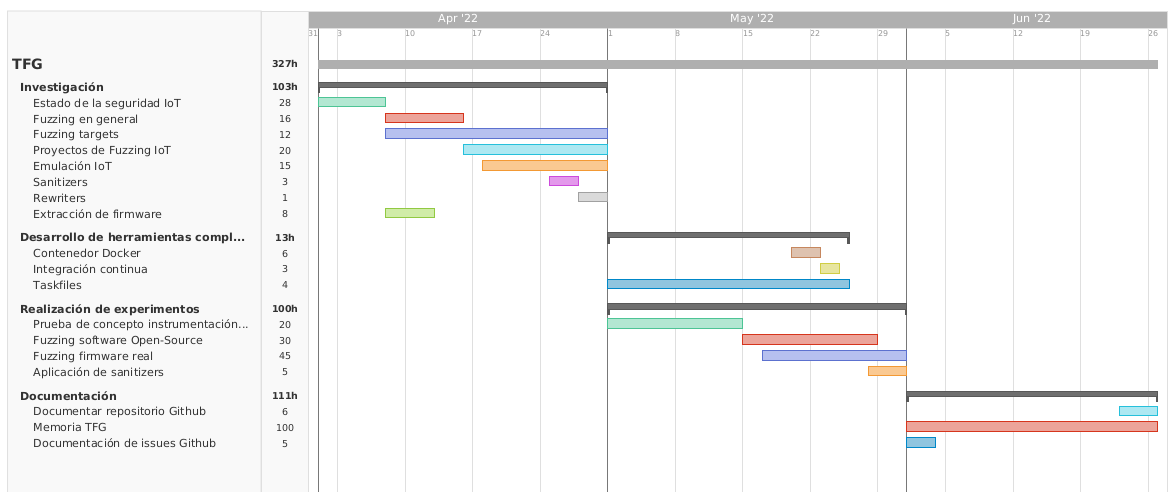
\includegraphics[scale=0.3]{Gantt.png}}
    \caption{Diagrama de Gantt con la planificación preliminar del proyecto.}
    \label{fig:gantt}
\end{figure}

La realización del proyecto se reparte en tres meses durante los cuales se plantean una serie de tareas generales a completar,
agrupadas en cuatro categorías principales, ''Investigación'', ''Desarrollo de herramientas complementarias'', ''Realización de 
experimentos'' y ''Documentación''. El siguiente listado de tareas queda reflejado en \ref{fig:gantt}:
\begin{itemize}
    \item \textbf{Investigación}: 
    \begin{itemize}
        \item \textbf{Estado de la seguridad IoT}: Como primera tarea del proyecto se ha de investigar la situación actual de la seguridad
        en el campo del internet de las cosas para tener un punto de partida.
        \item \textbf{Fuzzing en general}: Es necesario investigar el funcionamiento de la técnica del fuzzing en sí antes de proceder a 
        investigar sobre su aplicación al campo del IoT.
        \item \textbf{Fuzzing targets}: Se investigarán distintos dispositivos y sus respectivos firmwares para descubrir software de interés
        sobre el que realizar fuzzing.
        \item \textbf{Proyectos de fuzzing IoT}: Como parte del estudio del estado del arte se investigarán las distintas técnicas y herramientas 
        aplicadas actualmente en la materia.
        \item \textbf{Emulación IoT}: Dado que la emulación es un factor clave en el fuzzing IoT será necesario profundizar en las distintas 
        técnicas disponibles.
        \item \textbf{Sanitizers}: Los sanitizers o desinfectantes suelen ser utilizados para agilizar el proceso de fuzzing. Debemos de investigar cómo difiere
        su aplicación en dispositivos IoT con respecto a su uso tradicional.
        \item \textbf{Rewriters}: Investigar sobre esta nueva técnica que puede aumentar la eficiencia del fuzzing instrumentando estáticamente binarios.
        \item \textbf{Extracción de firmware}: Como paso previo a aplicar fuzzing es necesario obtener los binarios que serán objeto de
        experimento. Investigaremos la metodología actual para extraer firmware y los binarios incluidos en este.
    \end{itemize}
    \item \textbf{Desarrollo de herramientas complementarias}:
    \begin{itemize}
        \item \textbf{Contenedor Docker}: Querremos desarrollar un contenedor Docker que evite tener que lidiar con la gran cantidad de dependencias 
        y paquetes software necesarios para realizar fuzzing orientado a IoT.
        \item \textbf{Integración continua}: Se automatizará la publicación del contenedor Docker a DockerHub mediante CI/CD.
        \item \textbf{Taskfiles}: Aplicando también los conocimientos obtenidos en la asignatura de IV, se hará uso de un gestor de tareas que 
        facilitará la reproducibilidad de los experimentos. 
    \end{itemize}
    \item \textbf{Realización de experimentos}:
    \begin{itemize}
        \item \textbf{Prueba de concepto instrumentación dinámica}: Como introducción al fuzzing IoT, crearemos una prueba de concepto sobre
        un binario simple que nos permita familiarizarnos con las herramientas utilizadas y conocer las capacidades de la instrumentación dinámica.
        \item \textbf{Fuzzing software Open-Source}: Una vez se ha ganado algo de soltura con las herramientas a utilizar, se aplicará fuzzing 
        sobre un proyecto de código abierto orientado a sistemas empotrados.
        \item \textbf{Fuzzing firmware real}: Se llevará a cabo un experimento donde se aplique fuzzing a binarios extraídos del firmware de un 
        dispositivo real con el fin de identificar una vulnerabilidad conocida. 
        \item \textbf{Aplicación de sanitizers}: Para finalizar, se hará uso de desinfectantes para analizar de qué forma 
        su uso influye en el proceso de fuzzing.
    \end{itemize}
    \item \textbf{documentación}:
    \begin{itemize}
        \item \textbf{Documentar repositorio Github}: El repositorio donde llevar a cabo el control de cambios del proyecto será 
        adecuadamente documentado a través de la redacción de diversos READMEs para sus distintas secciones.
        \item \textbf{Documentación de issues Github}: Dado que van a usarse diversas herramientas de código abierto activamente 
        desarrolladas a día de hoy, será necesario documentar a través de issues en los repositorios de proyecto correspondientes
        los distintos fallos de software que se encuentren en estos durante la realización de los experimentos.
        \item \textbf{Memoria TFG}: Todo el desarrollo del proyecto de principio a fin deberá de quedar reflejado en una memoria final.
    \end{itemize}
\end{itemize}

\section{Estimación de costes}
Previamente a comenzar con el proyecto, estimaremos los costes de su realización en base a diferentes factores como el número estimado de horas necesarias, el sueldo medio de un ingeniero informático junior, los costes del hardware que necesitaremos para llevarlo a cabo o servicios necesarios
que también necesitan ser sufragados como internet o la electricidad utilizada.\bigskip

Empezamos partiendo del dato de las 327 horas estimadas en el diagrama de Gantt (figura \ref{fig:gantt}) durante 3 meses.
De esta cifra descontamos el número de horas dedicado al aprendizaje personal e investigación llevados a cabo durante el primer mes del
proyecto y utilizaremos el número de horas restantes para realizar una estimación de los costes de este proyecto. Respecto al coste de la 
mano de obra, teniendo en cuenta un 
salario medio de ingeniero informático junior de 20.000 euros brutos al año y que para llevar a cabo el proyecto se planea dedicar una media de 
4 horas diarias durante todos los días de la semana, podemos calcular un coste de $\sim13'7\euro$ la hora. Los costes de hardware se limitan al
ordenador sobre el que se va a realizar el proyecto, ya que al basar este en técnicas de emulación no va a ser requerido hardware adicional 
como podrían ser dispositivos IoT de domótica sobre los que aplicar el fuzzing. El fuzzing no requiere de ningún hardware específico para el 
ordenador con el que se va a realizar, aunque si ayuda considerablemente el tener suficiente RAM e hilos de CPU para poder aumentar el número de ejecuciones por segundo 
poniendo en marcha varias instancias en paralelo del fuzzer. Un ordenador de sobremesa como el que va a ser utilizado con 16GB de RAM, un 
Ryzen 5 3600 de 6 núcleos y 12 hilos junto con una GPU cualquiera (exclusivamente utilizada como salida de vídeo, ya que el Ryzen 5 3600 carece de GPU integrada) puede ser
conseguido por $\sim600\euro$.

Por último, el coste del servicio de internet en el lugar de trabajo actualmente es de $30\euro$ mensuales mientas 
que el coste de la luz es difícil de estimar debido a las constantes fluctuaciones en el precio de la electricidad, aunque estimaremos que 
para un un ordenador de dichas características que en el peor de los casos con la CPU trabajando al 100\% consume $\sim400W$ junto a sus 
periféricos, se produce un gasto de 1'6 KWh para 4 horas diarias de trabajo. Esto se traduce a $\sim0'37\euro$ diarios ($10'36\euro$ mensuales)
con un precio de $0'23\euro$ el KW/h. Generamos la siguiente tabla con el presupuesto estipulado:

\begin{table}[H]
    \begin{tabular}{llll}
    \rowcolor[HTML]{C0C0C0} 
    \textbf{Descripción}           & \textbf{Uds.} & \textbf{Precio/Unidad ($\euro$)} & \textbf{Total ($\euro$)} \\
    Mano de obra                   & 224           & 13'70                  & 3.068'80               \\
    Ordenador de sobremesa         & 1             & 600                    & 600                    \\
    Servicio de internet (mensual) & 2             & 30                     & 60                     \\
    Servicio de luz (mensual)      & 2             & 10'36                  & 20'72                  \\\hline
                                   &               & \textbf{Total sumado:} & 3.749'52$\euro$              
    \end{tabular}
    \caption{Presupuesto para la realización del proyecto.}
    \label{table:presupuesto}
\end{table}

Como conclusión comentar que no se trata de un presupuesto competitivo para la labor de investigación que se desea realizar. Estas tareas suelen 
ser llevadas a cabo por expertos de la materia a tratar mientras que este proyecto fue planteado para ser llevado a cabo sin experiencia previa al 
respecto con el objetivo de aprender en el proceso. Es por ello que tareas que podrían ser realizadas en menor tiempo por un investigador ya formado previamente, se prolongan 
en el tiempo con el consecuente incremento en costes.

\section{Seguimiento del desarrollo}
\label{seguimiento}
Github ha sido la plataforma de control de cambios elegida debido a que junto con Git, han sido ampliamente utilizados
en las distintas asignaturas del grado de Ingeniería Informática y ya se parte conociendo su funcionamiento y dinámica de 
trabajo. Github proporciona una funcionalidad de tablero Kanban (Figura \ref{fig:kanban}) que combinado con lo comentado en ''\nameref{metodologia}''
nos permite de un vistazo ver el estado actual de las tareas del proyecto mediante su clasificación en una serie de columnas 
definidas que agrupan las issues según si se tratan de issues por comenzar, issues en progreso, issues bloqueadas a espera 
de arreglos en software de terceros o issues completadas. Podemos observar un ejemplo de issue creada durante la realización de los 
experimentos planteados en la figura \ref{fig:issue}.
\begin{figure}[H]
    \centering{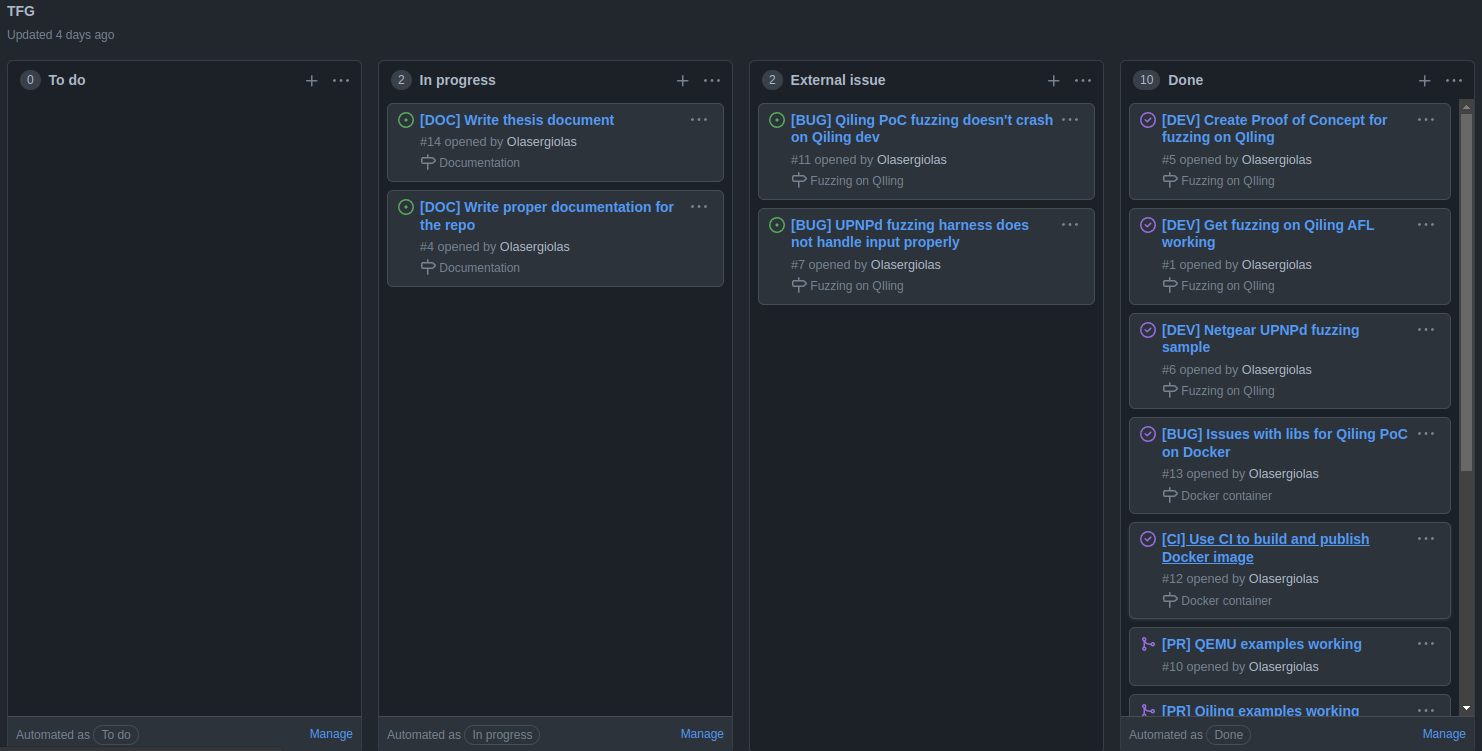
\includegraphics[scale=0.2]{kanban.png}}
    \caption{Funcionalidad de tablero Kanban de Github.}
    \label{fig:kanban}
\end{figure}

\begin{figure}[H]
    \centering{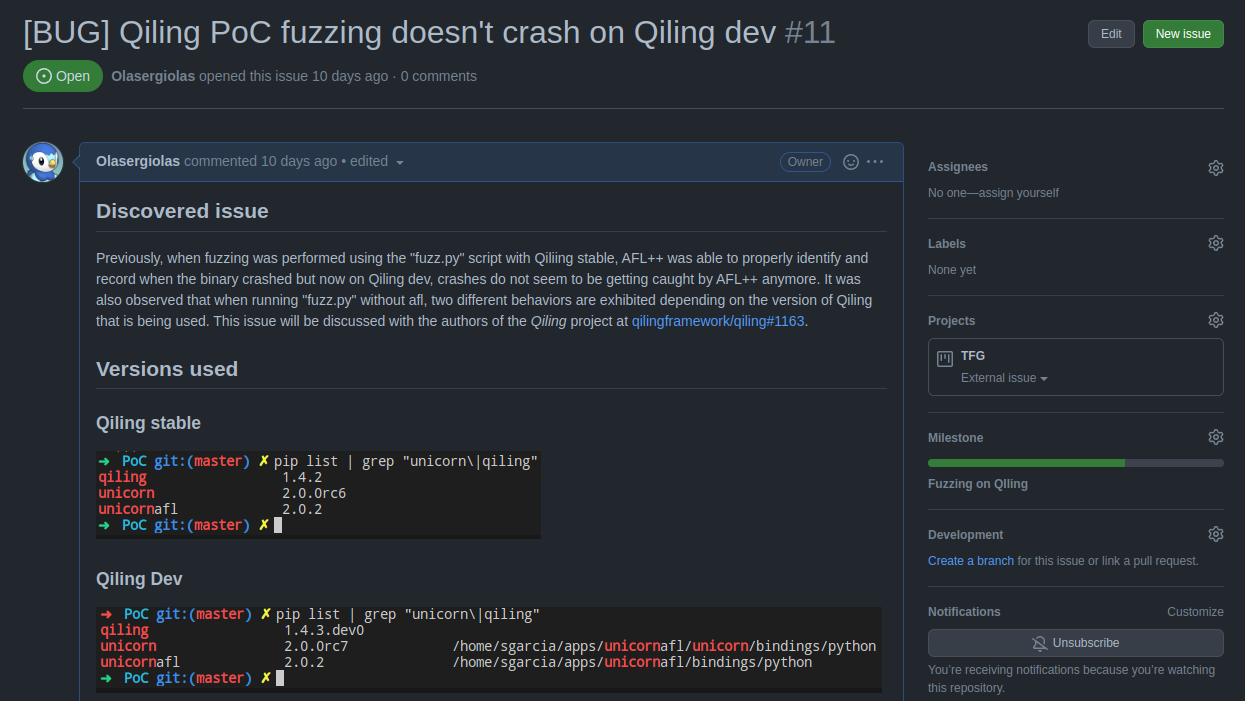
\includegraphics[scale=0.24]{issue.png}}
    \caption{Emisión de \href{https://github.com/Olasergiolas/TFG/issues/11}{informe} de error software en el repositorio del proyecto.}
    \label{fig:issue}
\end{figure}

Todo el contenido de este proyecto estará disponible públicamente en el siguiente repositorio de Github \href{https://github.com/Olasergiolas/TFG}{https://github.com/Olasergiolas/TFG}. 

	
	\chapter{Herramientas complementarias}
\label{herramientas}
\section{Introducción}
En este capítulo trataremos muy brevemente las dos herramientas que han sido implementadas con el objetivo de facilitar el proceso de llevar a cabo los 
experimentos que hemos comentado. Aún no teniendo relación directa con la temática que estamos tratando, estas herramientas complementarias no solo 
hacen nuestra labor más sencilla sino que también ayudan enormemente a todo aquel que esté interesado en reproducir el trabajo realizado en este proyecto
o incluso en poner en práctica nuevos experimentos. Con este objetivo, se decide hacer uso de un gestor de tareas y de un contenedor Docker cuyos contenidos estarán
publicados junto con el resto del proyecto en nuestro repositorio de Github.

\section{Contenedor Docker e integración continua}
Dado que todo lo relacionado con trabajar con binarios de arquitecturas distintas puede suponer un reto a la hora de gestionar todas las dependencias
y paquetes requeridos, se decide crear un contenedor Docker que contenga todo lo necesario para compilar, depurar y fuzzear binarios de arquitecturas como 
ARM o MIPS. En primer lugar recopilamos un listado de herramientas que pudiéramos querer incluir en el contenedor como pueden ser toolchains de arquitecturas
usadas en dispositivos IoT, 
fuzzers como Radamsa y AFL++ o algunos frameworks de instrumentación dinámica como Unicorn o Qiling. En segundo lugar, decidimos sobre qué
imagen basar nuestro contenedor. Principalmente, la decisión se dividía entre expandir la imagen oficial de AFL++ o hacer uso de la imagen de Ubuntu (focal), pero se 
terminó optando por la segunda opción ya que aunque la imagen de AFL++ viene pre-instalada con un gran número de herramientas que nos son de utilidad, el 
estar basada en una versión tan reciente de Ubuntu (22.04 Jammy) hace que incluya paquetes y librerías actualmente incompatibles con algunas de las 
herramientas discutidas. Además, aplicaremos los conocimientos obtenidos en la asignatura de ''Infraestructura Virtual'' para automatizar la publicación de nuestro
contenedor a DockerHub siempre que se realice un cambio sobre el fichero Dockerfile en la rama principal del repositorio mediante Github Actions,
el sistema de integración continua de Github.

\section{Gestión de tareas con Task}
Debido a la complejidad y al gran número de órdenes que será necesario utilizar durante los experimentos, decidimos dejarlas reflejadas a modo de tareas
en ficheros locales. Estos ficheros serán luego interpretados por un gestor de tareas que se encargará de poner en marcha otras tareas sobre las que haya 
dependencia además de ejecutar todos los comandos asociados a la tarea. Para esto, usamos Task\cite{task} una alternativa moderna a GNU make escrita en Go con una sintaxis más 
amigable. Generaremos un fichero Taskfile.yml por cada experimento, los cuales incluirán tareas para llevar a cabo acciones como el compilado de código,
la configuración del entorno de fuzzing o la puesta en marcha de emuladores.

	
	\chapter{Experimentos}
\label{experimentos}
A lo largo de esta sección, se tratarán de forma detallada los distintos experimentos que se han realizado para este proyecto con el fin de 
poner en práctica los conocimientos obtenidos durante el proceso de investigación de la materia. Para los experimentos se planteará cuál es el 
objetivo a alcanzar y los posibles enfoques a aplicar para llegar a una solución, además de tratar los retos encontrados por el camino, los 
resultados del experimento y las lecciones que puedan ser aprendidas de este.

\section{Introducción al uso de Qiling: Prueba de concepto y fuzzing}
\subsection{Introducción al experimento}
En la sección de ''\nameref{estado_del_arte}'' decíamos que hay ciertos casos para los que no nos interesa fuzzear la ejecución de principio a fin 
de un programa como por ejemplo cuando hacemos frente a un software complejo y costoso en tiempo de ejecutar o cuando para ejecutarlo correctamente necesitamos de algún periférico o recurso del que carecemos. Además, la idea de poder dirigir el proceso de fuzzing a los componentes del código que más nos 
resulten de interés es de alto valor para nuestro principal objetivo al realizar fuzzing, la identificación de vulnerabilidades en el menor tiempo posible.
Frameworks de emulación como Unicorn o Qiling hacen esto posible gracias a sus capacidades no solo de emulación sino también de instrumentación dinámica de binarios.
Cuando se decidió poner en práctica esta técnica para realizar fuzzing orientado a IoT, fue necesario elegir entre estos dos proyectos, los cuales 
representan a día de hoy los principales framework multi-arquitectura centrados en la instrumentación dinámica a través de una API. Qiling terminó siendo 
la elección final gracias a que además de presentar toda la funcionalidad de Unicorn, nos permite trabajar a más alto nivel con conceptos como librerías dinámicas,
llamadas al sistema o I/O, al contrario que este otro que solo trabaja a nivel de instrucciones de CPU.\bigskip

El objetivo de este pseudo-experimento es servir de una breve toma de contacto práctica con las capacidades del framework de Qiling, para facilitar la comprensión 
del siguiente experimento a realizar, donde usaremos Qiling entre otras herramientas para analizar una vulnerabilidad real recientemente descubierta en un router
inteligente. Llevar a cabo esta toma de contacto inicial resulta de gran ayuda ya que aunque el código que vamos a emular y fuzzear a continuación 
no pertenece a un caso real, puede resultar abrumador intentar introducirnos directamente en el mundo de la instrumentación dinámica sobre binarios encontrados en 
imágenes firmware de dispositivos IoT reales debido a su complejidad. Por ello,empezaremos instrumentando un simple ejemplo de código creado por nosotros mismos que 
buscará simular comportamientos problemáticos comúnmente encontrados al realizar fuzzing de binarios de dispositivos empotrados/IoT reales.\bigskip

Más concretamente, este pseudo-experimento a modo de prueba de concepto consistirá en la emulación y fuzzing mediante Qiling de un simple binario que tras 
dormir durante cinco segundos lleva a cabo el ''cifrado'' de un string introducido como parámetro mediante la aplicación de una operación
XOR a cada byte del string. El tiempo durante el cual el binario duerme intenta simbolizar escenarios problemáticos reales de cara al fuzzing 
como la ejecución de rutinas de código previas a la funcionalidad que queremos evaluar o los posibles bloqueos parciales o completos de la ejecución ocasionados por no conseguir emular el entorno de ejecución real a la perfección. En cualquiera de los casos, este tipo de comportamientos dificulta
enormemente el obtener buenos resultados a través del fuzzing tradicional como probaremos a continuación.

\subsection{Realización del experimento}
Empezaremos por desarrollar un simple código en C que implemente la funcionalidad descrita anteriormente. Además, añadiremos a la función de 
cifrado de strings un crash forzado por una lectura de array fuera de límites que se dará cuando el string introducido empiece por el carácter
'a' y tenga una longitud mayor que diez caracteres. Esto nos servirá para evaluar la efectividad de nuestra solución de fuzzing para dar con 
el input que origina este crash. El código mostrado a continuación será compilado para ARM, que como ya sabemos se trata de una arquitectura 
comúnmente encontrada en dispositivos IoT y lo haremos usando compilación cruzada con el toolchain de GNU para ARM.

\begin{lstlisting}[language=C, caption=Código de ejemplo a fuzzear., captionpos=b,
    frame=single, breaklines, showstringspaces=false]
    #include <stdio.h>
    #include <unistd.h>
    #include <string.h>
    #include <stdlib.h>

    void printRes(char str[], unsigned len){
        printf("Ciphered output: ");
        for (unsigned i = 0; i < len; ++i)
            printf("\\x%02X", str[i]);
        printf("\n");
    }

    void processArgs(char str[]){
        unsigned len = strlen(str);
        
        if (len > 10 && str[0] == 'a'){
            printf("CRASH");
            char dst[2];
            dst[6] = str[0];
        }

        for (unsigned i = 0; i < len; ++i){
            str[i] = (char)(str[i] ^ 'c');
        }

        printRes(str, len);
    }

    int main(int argc, char* argv[]){
        if (argc != 2){
            printf("Usage: %s <input_string>\n", argv[0]);
            exit(1);
        }
        
        sleep(5);
        processArgs(argv[1]);
    }
\end{lstlisting}

\subsubsection{Intento de fuzzing mediante AFL++ en modo QEMU}
Con el fin de ejemplificar como un comportamiento como este puede resultar desastroso de cara a fuzzear un binario, intentamos fuzzear el 
código mostrado mediante técnicas más tradicionales como puede ser el uso de AFL++ en su modo QEMU (emulación user-mode). Este modo de AFL++ es el 
modo por defecto recomendado cuando se desea hacer fuzzing sobre un binario que no ha sido instrumentado. Para ello, preparamos un input 
básico con la cadena ''BBBBBB'' e iniciamos el fuzzing (figura \ref{fig:QEMUPoC}) con la siguiente orden (Fijamos la variable de entorno
''QEMU\_LD\_PREFIX'' a la ruta que contiene las librerías necesarias en tiempo de ejecución, -Q indica a AFL++ que ha de usarse el modo QEMU y
-t el valor del timeout en milisegundos el cual deberá ser mayor que el valor utilizado en la llamada a \textit{sleep}):

\begin{lstlisting}[language=bash]
    $ QEMU_LD_PREFIX=/usr/arm-linux-gnueabi afl-fuzz -i fuzz_setup/in -o fuzz_setup/out -Q -t 7000 -- ./bin/main_arm @@
\end{lstlisting}

\begin{figure}[H]
    \centering
    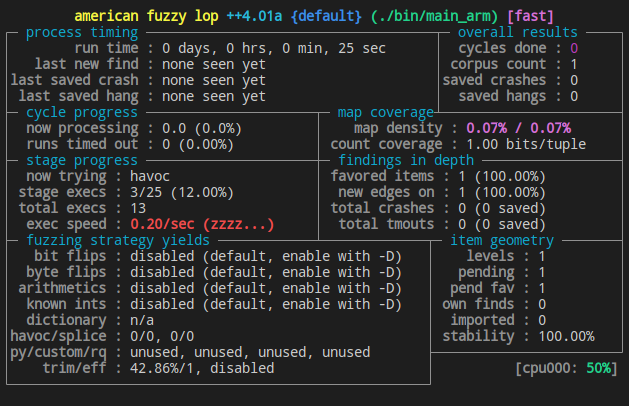
\includegraphics[scale=0.59]{QEMUPoC.png}
    \caption{AFL++ fuzzeando código problemático en modo QEMU.}
    \label{fig:QEMUPoC}
\end{figure}

Observando la información reportada por AFL++, salta a la vista que el número de ejecuciones por segundo (0.2/s en la figura \ref{fig:QEMUPoC}) es demasiado bajo como para encontrar 
el crash que buscamos en un tiempo razonable y por ello, procedemos a hacer uso de técnicas alternativos como Qiling para solucionarlo.

\subsubsection{Uso de Qiling}
Qiling proporciona funciones en su API para llevar a cabo diversas tareas de instrumentación dinámica que pueden sernos de utilidad en este 
tipo de casos en los que métodos más tradicionales de fuzzing pueden no ser viables. Ejemplos de funcionalidades interesantes son los snapshots,
que pueden acelerar el fuzzing guardando el estado de la CPU y la memoria en un momento dado y restaurarlo para cada iteración, las operaciones 
con memoria y registros, que nos permiten trabajar con los parámetros de las funciones, los hooks, que hacen posible ejecutar código propio al 
llegar a una dirección del programa específica o el mapeo de dispositivos del host al entorno de emulación. De todo esto haremos uso de las 
operaciones con memoria y registros de la CPU para modificar el punto de entrada del binario a la función de cifrado que deseamos fuzzear e 
instrumentar, además de usar hooks para automáticamente realizar dichas operaciones al alcanzar puntos estratégicos del binario durante la 
ejecución.\bigskip

Dado que estamos ante un binario simple, su emulación con Qiling no requiere de ninguna instrumentación adicional. Para emular el binario 
hacemos uso de ''qltool'', la herramienta proporcionada por Qiling para emular rápidamente binarios sin aplicar instrumentación. Utilizamos la 
siguiente orden usando ''abc'' como cadena de entrada y observamos como el binario compilado para ARM se ejecuta correctamente, mostrando tras cinco segundos de espera los
bytes de la cadena resultante en hexadecimal (figura \ref{fig:qltool}).

\begin{lstlisting}[language=bash]
    $ qltool run --rootfs /usr/arm-linux-gnueabi -f bin/main_arm --args abc
\end{lstlisting}

\begin{figure}[H]
    \centering
    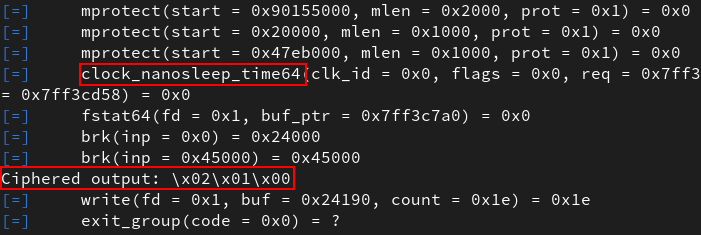
\includegraphics[scale=0.59]{qltool.png}
    \caption{Emulación de código ARM con qltool.}
    \label{fig:qltool}
\end{figure}

Ahora, para aplicar fuzzing consiguiendo buenos resultados necesitaremos hacer uso de instrumentación dinámica que nos permita saltar esa pausa que 
simula una sección de código problemática. Para esto, crearemos un script de Python en el que haremos uso de la API de Qiling para modificar
el flujo de ejecución del binario y usar como ''main'' del programa la función de cifrado de cadenas de texto. Como fuzzer a utilizar junto a Qiling, 
haremos uso de AFL++ gracias a su fácil integración con Unicorn y Qiling a través de Unicornafl lo cual nos permitirá realizar fuzzing aprovechando la 
información de cobertura de código proporcionada por Qiling. Además, ya que durante el fuzzing 
no nos interesa que la cadena resultante se muestre por pantalla, también podemos finalizar la ejecución en la dirección donde se encuentre la instrucción
de retorno de la función ''processArgs()'', reduciendo así el número de instrucciones a ejecutar. En la figura \ref{fig:QilingFuzzDiagram} observamos el
flujo de ejecución que se desea llevar a cabo para fuzzear el código.

\begin{figure}[H]
    \centering
    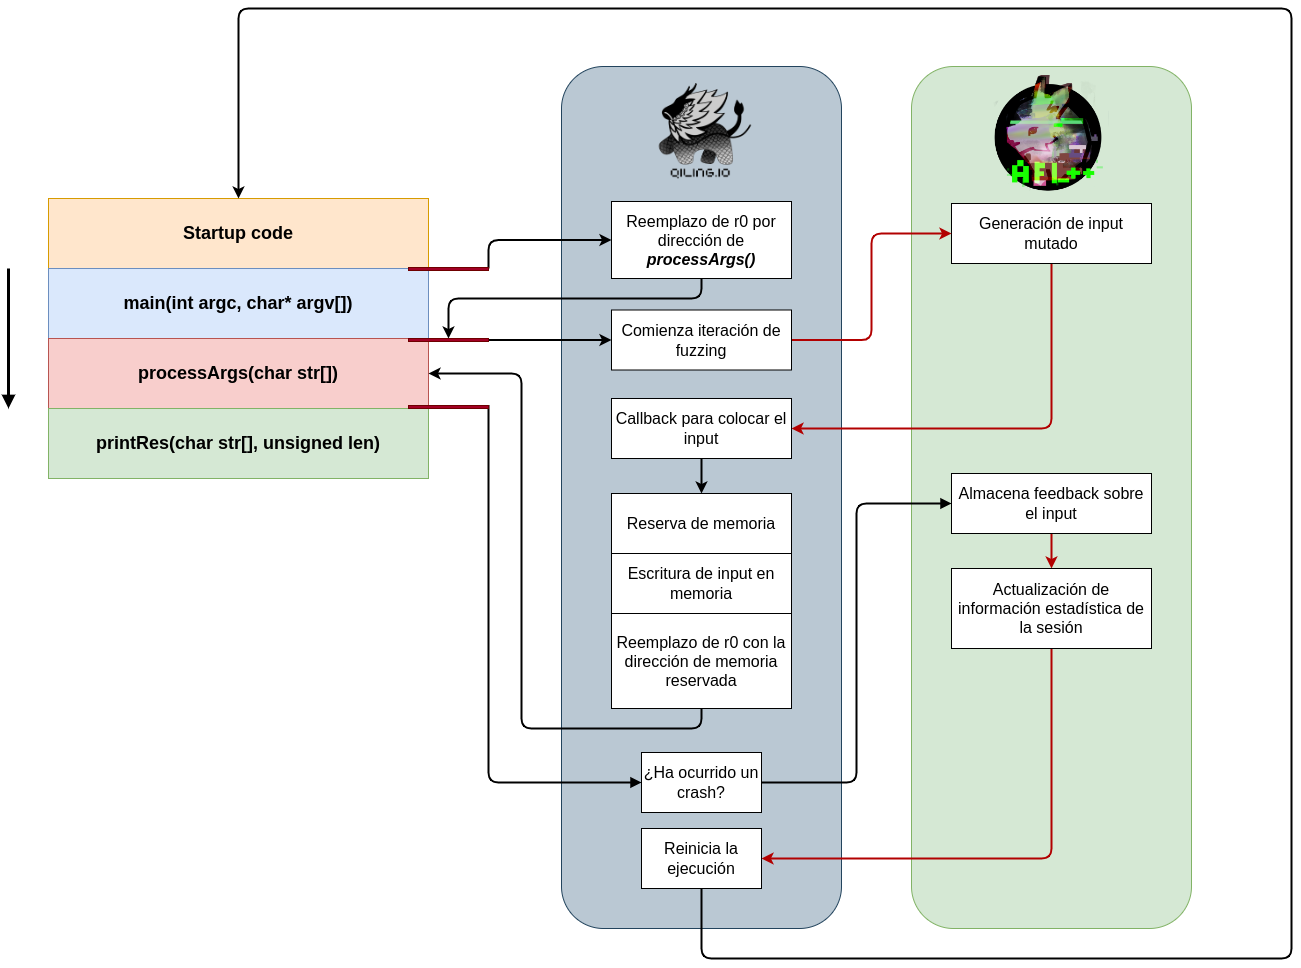
\includegraphics[scale=0.26]{QilingFuzzDiagram.png}
    \caption{Diagrama simplificado del proceso de fuzzing a implementar en Qiling.}
    \label{fig:QilingFuzzDiagram}
\end{figure}

Para llevar a cabo el diagrama mostrado, empezamos estableciendo el hook y el callback que cambie el punto de entrada de ''main()'' por ''processArgs()''.
La API de Qiling ofrece la función ''hook\_address(callback, trigger\_address)'' que toma como parámetros la función de Python a llamar a modo de callback 
y la dirección de una instrucción dentro del binario para la cual llamar al callback previamente a su ejecución. La dirección elegida para fijar el callback 
será la de la llamada a ''\_\_libc\_start\_main()'' como parte del proceso de setup realizado por el binario previamente a ejecutar su main. El callback
simplemente usará la función ''ql.arch.regs.write(register\_id, value)'' de la API de registros de CPU de Qiling para fijar el valor del registro R0 a la dirección de la primera 
instrucción de ''processArgs()''. Lo que se consigue modificando R0 es alterar el primer parámetro de la llamada a una función en ARM32. Aplicamos esta
técnica en lugar de fijar directamente el contador de programa a la primera instrucción de ''processArgs()'' para conservar el código 
de inicialización del entorno de ejecución y evitar así diversos problemas como errores de enlazado de librerías dinámicas.\bigskip

Por último, integramos la ejecución de la función con AFL++ mediante un hook adicional que inicie la iteración de fuzzing y un callback que pueda ser 
llamado por AFL++ para introducir el input mutado en memoria. En el snippet de código mostrado a continuación vemos también como el callback ha de 
reservar y escribir en memoria los bytes del input ya que la función a fuzzear utiliza un string como parámetro.

\begin{lstlisting}[language=python, caption=Integración de AFL++ con nuestro script de Qiling., captionpos=b,
    frame=single, breaklines]
    ...
    def place_input_callback(_ql: Qiling, input: bytes, _):
        address = _ql.mem.map_anywhere(len(input))
        _ql.mem.write(address, input)
        _ql.arch.regs.write("r0", address)

    def start_afl(_ql: Qiling):
        ql_afl_fuzz(_ql, param_file, place_input_callback, exits=[ql.os.exit_point])

    ql.hook_address(start_afl, TARGET_FUNC_ADDR)

    ...
\end{lstlisting}

Para comenzar la sesión de fuzzing utilizamos como input inicial un fichero con la cadena ''BBBBBB'' y la siguiente orden para 
indicar a AFL++ que utilice nuestro script en modo Unicorn (figura \ref{fig:QilingPoCfuzz}). 

\begin{lstlisting}[language=bash]
    $ afl-fuzz -i fuzz_setup/in -o fuzz_setup/out -U -- python3 src/fuzz.py @@
\end{lstlisting}

\begin{figure}[H]
    \centering
    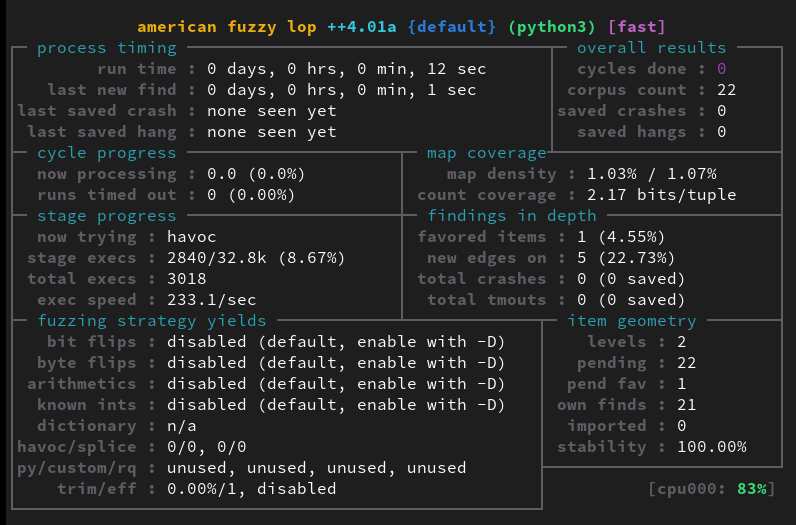
\includegraphics[scale=0.40]{QilingPoCfuzz.png}
    \caption{Prueba de concepto de fuzzing con Qiling y AFL++.}
    \label{fig:QilingPoCfuzz}
\end{figure}

\subsection{Resultados}
Hemos podido comprobar que el fuzzing de nuestro código de prueba utilizando AFL++ en modo QEMU ha resultado ser un fracaso en términos de 
eficiencia como era de esperar. En cambio,
al aplicar técnicas de instrumentación dinámica en Qiling hemos conseguido una mejora abismal en el número de ejecuciones por segundo durante el fuzzing, 
yendo de menos de una ejecución por segundo en QEMU a alrededor de doscientas con Qiling. Pasando a la detección de la vulnerabilidad introducida, 
cabe mencionar que hubo problemas para registrar correctamente los crashes producidos en Qiling. Tras un poco de investigación, parece ser que Qiling en su versión developer
(recomendada en la documentación oficial frente a la estable) ha sufrido una regresión en el tratamiento de crashes ya que Qiling estable es capaz de 
reportar a AFL++ cuando nuestro código crashea debido a lectura fuera de límites introducida, mientras que en su versión developer el crash no es reportado.
Tras crear una \href{https://github.com/qilingframework/qiling/issues/1163}{issue} en el repositorio oficial de Qiling\cite{qiling}, el bug ha sido reconocido y está siendo corregido actualmente.


\subsection{Lecciones aprendidas}
A través de la realización de esta pequeña prueba de concepto ha quedado patente el potencial de Qiling cuando se trata de llevar a cabo tareas relacionadas
con la instrumentación dinámica de binarios, como es el fuzzing. Teniendo en cuenta que este ejemplo se trata solo de una pequeña toma de contacto con la herramienta
para introducirnos a su uso, donde realmente aprenderemos sobre casos prácticos reales de aplicación de Qiling es en el experimento a continuación.

\section{Identificación de vulnerabilidad real a través de fuzzing: Netgear R7000}\label{r7000_section}
\subsection{Introducción al dispositivo}
El Netgear R7000, también conocido como Nighthawk AC1900 es un router WIFI ''inteligente'' lanzado al mercado originalmente en 2013 con una última
revisión del hardware en 2018 que sigue en venta actualmente. Este producto de la gama de routers premium de Netgear recibe actualizaciones periódicas
a día de hoy por parte del fabricante y se trata de una elección muy popular entre aquellos consumidores que buscan un router dual-band de altas prestaciones. 
\begin{figure}[H]
    \centering
    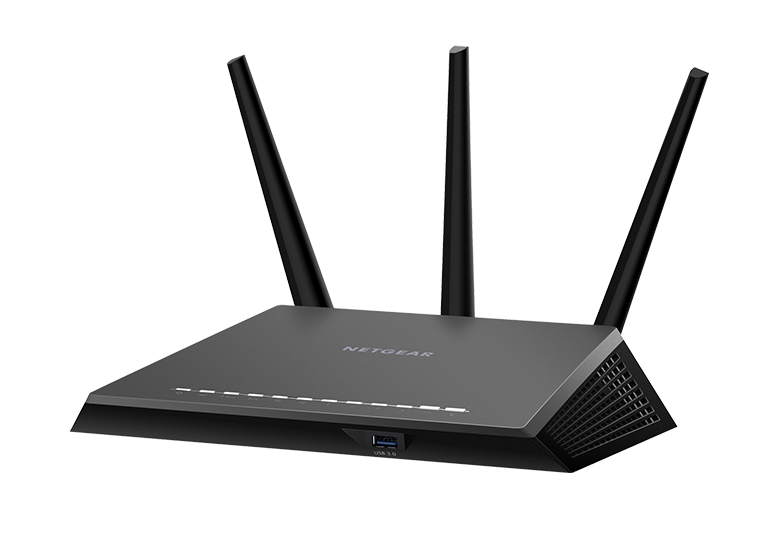
\includegraphics[scale=0.30]{r7000.png}
    \caption{Netgear R7000 (Nighthawk AC1900).}
    \label{fig:r7000}
\end{figure}

\subsection{Recopilación de información}
Consultando sus especificaciones técnicas principales 
encontramos que posee una CPU de 1GHz dual-core, 256MB de RAM, 128MB de memoria flash y soporte para dual-band de 2'4GHz a 600Mbps y de 5GHz a 
1300Mbps. Aunque estas especificaciones son interesantes a la hora de conocer cómo de restringido respecto a rendimiento está el dispositivo,
no son lo suficientemente detalladas como para aportarnos información clave que necesitamos conocer para aplicar emulación sobre este.
Principalmente, desconocemos el procesador que está siendo utilizado y su arquitectura, ya que el fabricante no proporciona dicha información.
Cuando nos encontramos en esta situación en la que deseamos conocer información más detallada sobre los componentes internos de un dispositivo, 
una posible solución es consultar su informe de aceptación para la certificación del FCC\cite{fcc} en la base de datos \hyperlink{fccid.io}{fccid.io}.
El FCC es un organismo de certificación encargado de evaluar todo producto que vaya a ser comercializado en los Estados Unidos que emita 
radiofrecuencias con el fin de asegurar que dichos dispositivos no produzcan interferencias dañinas que pudieran afectar al correcto
funcionamiento de otros dispositivos como equipamiento médico, aeronáutico o sistemas de telecomunicaciones.\bigskip

Accediendo a la base de datos podemos encontrar información de los reportes que se han ido realizando sobre las distintas iteraciones del producto,
concretamente, el reporte de mayor interés para nuestra tarea es el titulado ''Internal Photos'' publicado para la revisión lanzada en 2018\cite{netgearFCCid}.
Buscando lo que pudiera ser la CPU principal nos llaman la atención dos chips mostrados en el informe. El primero (figura \ref{fig:r7000transceptor}), al 
consultar la ficha técnica del BCM4360 descubrimos que se trata de un transceptor WIFI del fabricante Broadcom, por lo tanto no es lo que tratamos de 
encontrar. Respecto al segundo chip (figura \ref{fig:r7000cpu}), consultando las especificaciones presentes en la ficha técnica del Netgear R7000 
(tabla \ref{table:r7000}) proporcionada por OpenWRT podemos ver que se trata de un System on a Chip (SoC) WIFI lanzado al mercado en 2013\cite{broadcomSOCs} 
que en su interior contiene un procesador dual core ARM Cortex A9 de 32 bits.

\begin{figure}[H]
    \centering
    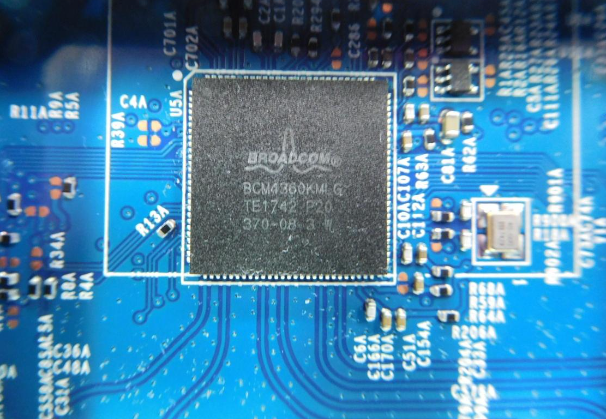
\includegraphics[scale=0.45]{r7000transceptor.png}
    \caption{Broadcom BCM4360 en el interior del Netgear R7000.\cite{netgearFCCid}}
    \label{fig:r7000transceptor}
\end{figure}

\begin{figure}[H]
    \centering
    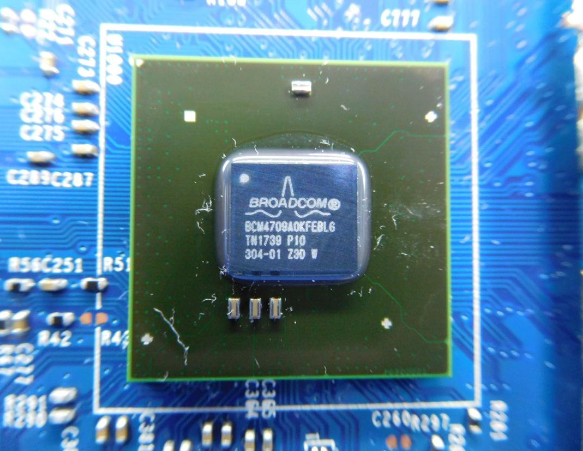
\includegraphics[scale=0.59]{r7000cpu.png}
    \caption{Broadcom BCM47 en el interior del Netgear R7000.\cite{netgearFCCid}}
    \label{fig:r7000cpu}
\end{figure}

\begin{table}[H]
    \centering
    \begin{tabular}{ |l|m{20em}| }
    \hline
    FCC ID                      & PY313200233                      \\\hline
    Industry Canada ID          & 4054A-13200233                   \\\hline
    Voltaje                     & 12 VDC, 3.5 A                    \\\hline
    CPU/SoC                     & Broadcom BCM4709A0 @1 GHz        \\\hline
    Arquitectura CPU            & ARM Cortex A9 (2 cores)          \\\hline
    Flash / RAM                 & 128 MiB / 256 MiB                \\\hline
    Chip WI1 \& WI2             & Broadcom BCM4360                 \\\hline
    Protocolos WI1 \& WI2       & an+ac / bgn                      \\\hline
    Configuración MIMO wireless & 3x3:3                            \\\hline
    Conector de antena          & U.FL, RP-SMA                     \\\hline
    Switch \& Ethernet          & Broadcom BCM4709A0               \\\hline
    Puertos WAN/LAN             & 1 / 4 (up to 1 Gb/s)             \\\hline
    Puertos USB                 & 1x USB 3.0, 1x USB 2.0           \\\hline
    Puerto serie                & 4-pin header, internal, 3.3V TTL \\\hline
    \end{tabular}
    \caption{Especificaciones del Netgear R7000.\cite{r7000datasheet}}
    \label{table:r7000}
\end{table}

Aunque Broadcom no proporciona una ficha técnica con las especificaciones del SoC, 
si que podemos consultar información más detallada sobre el Cortex A9 a través de la documentación oficial de ARM\cite{cortexA9}. Gracias a esto podemos 
conocer detalles como información sobre la Memory Management Unit (MMU) que utiliza la CPU. Esta información es de gran importancia ya que como explicaban
Muench et al.\cite{Muench2018}, la presencia de una MMU en un dispositivo empotrado puede alterar drásticamente el comportamiento de este ante corrupciones de 
memoria. Un dispositivo sin MMU puede no detectar fallas de memoria y seguir funcionando en un estado indefinido mientras que uno con MMU provoca un 
crash al detectar corrupción de memoria o la realización de alguna operación ilegal. Según la documentación oficial de la CPU, el procesador utiliza la MMU 
diseñada para la arquitectura Armv7, por lo que podemos deducir que un crash que encontremos aplicando fuzzing al firmware mediante emulación, podría ser replicado
en el dispositivo real.

\subsection{Obtención del firmware}
Una vez hemos recopilado información sobre el objeto de estudio, necesitaremos conseguir el firmware del dispositivo para proceder a su análisis y posterior 
emulación. A la hora de conseguir el firmware de un dispositivo IoT podemos enfrentarnos a una serie de retos dependiendo de cómo el fabricante distribuya
las imágenes del firmware. Podemos categorizarlos de la siguiente mantera:
\begin{itemize}
    \item \textbf{Medio de distribución}: En el mejor de los casos, el fabricante provee un enlace de descarga del firmware a través de su portal de soporte oficial. Aunque
    este suele ser el caso para dispositivos como routers o cámaras IP, no es común en otros dispositivos aún más limitados como bombillas inteligentes o asistentes de voz.
    También hay fabricantes que con el objetivo de intentar evitar que usuarios puedan aplicar técnicas de ingeniería inversa sobre los paquetes de actualización, integran 
    todo el proceso de actualización a través de una aplicación móvil o desde el propio dispositivo. Ante esto, es posible hacer uso de iptables para redirigir el tráfico
    de la aplicación o del dispositivo e intentar interceptar las peticiones al servidor de descargas de firmware. Por último, existe la posibilidad de que el fabricante no 
    haya provisto al dispositivo de un mecanismo de actualización para el usuario. Como último recurso, sería posible desmontar el dispositivo e intentar extraer el firmware 
    a través de la interfaz JTAG o leyendo los contenidos de la memoria EEPROM utilizando un programador (figura \ref{fig:programador}).
    \begin{figure}[H]
        \centering
        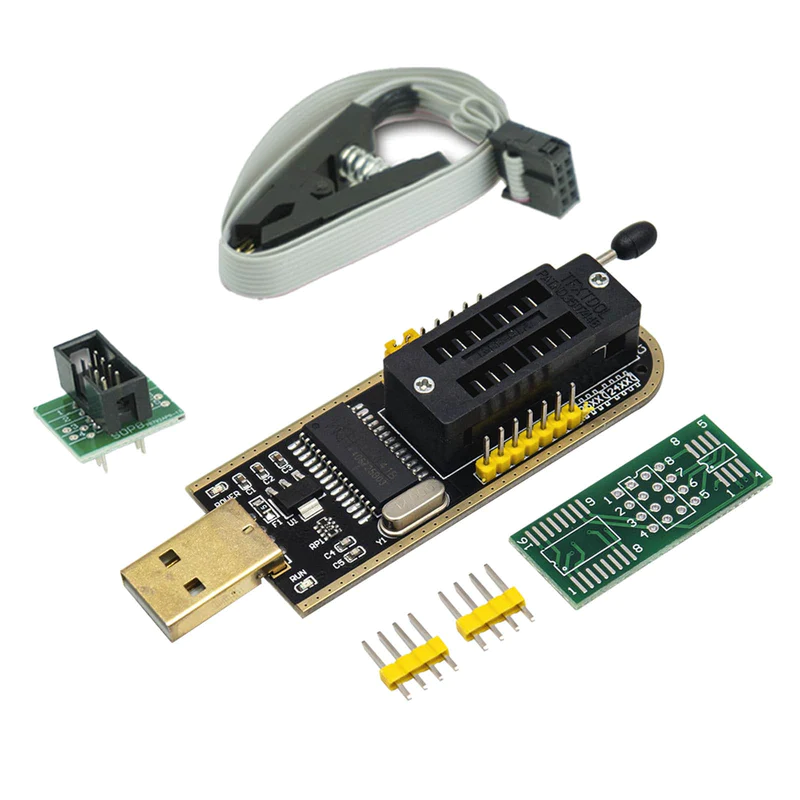
\includegraphics[scale=0.35]{programmer.png}
        \caption{Programador EEPROM CH341A genérico.}
        \label{fig:programador}
    \end{figure}
    \item \textbf{Cifrado}: Además de no proporcionar un portal de descargas de firmware, los fabricantes también suelen cifrar sus paquetes de actualización para dificultar las 
    tareas de análisis e ingeniería inversa. Dicho firmware es posteriormente descifrado por la rutina de actualización del dispositivo. Cuando se da este caso desgraciadamente 
    solo quedan dos opciones, o extraer el firmware del mismo dispositivo como se ha comentado en el punto anterior o intentar obtener la versión del firmware previa a que el 
    fabricante implementara el cifrado en las actualizaciones y aplicar ingeniería inversa sobre la rutina de descifrado del firmware para llevar a cabo nuestra propia implementación. 
    \item \textbf{Formato}: Es bastante común para los fabricantes distribuir sus paquetes de firmware en formatos propietarios difíciles de tratar sin software especializado. 
    Binwalk\cite{binwalk} es una herramienta que puede ayudar con el análisis y desenpaquetado de imágenes firmware en binarios de los cuales se desconoce su estructura. El uso de esta herramienta
    será tratado a continuación. También es posible que se den casos en los que binwalk no sea capaz de identificar o extraer correctamente el contenido de la imagen firmware, 
    teniendo que recurrir al diseño de herramientas específicas para el firmware con el que se está trabajando, identificando los offsets a partir de dónde empiezan los distintos 
    componentes de este y extrayéndolos manualmente con herramientas como dd de las coreutils de GNU.
\end{itemize}

Para el Netgear R7000, es posible obtener el firmware a través de su \href{https://www.netgear.es/support/product/r7000.aspx#download}{portal oficial de soporte}. Una vez 
descargado el paquete de firmware versión 1.0.11.128, procedemos a su análisis con la herramienta Binwalk. El primer paso es comprobar si el binario se encuentra cifrado mediante 
la comprobación de su entropía. La entropía del binario es un valor que representa el nivel de aleatoriedad entre los bytes del fichero y un valor alto constante
en todo el binario es un fuerte indicativo de que o su contenido ha sido comprimido o que este ha sido cifrado. Para consultar la entropía representada en una gráfica usamos Binwalk con la siguiente orden. 
\begin{lstlisting}[language=bash]
  $ binwalk -E R7000-V1.0.11.128_10.2.112.chk
\end{lstlisting}

Como podemos apreciar en la figura \ref{fig:binwalkEnt}, Binwalk reporta una entropía alta para el firmware. Para comprobar si estamos
ante un firmware cifrado intentamos identificar el contenido de este usando la flag ''-e'' en lugar de ''-E''. Al hacerlo, Binwalk es capaz de detectar 
la presencia de tres elementos dentro del firmware (figura \ref{fig:binwalkExt}), una primera entrada de nombre ''TRX firmware header'' que contiene metadatos
del firmware en formato TRX como un magic number, la versión de TRX en uso, longitud de la cabecera o un checksum CRC32 para comprobar la integridad del paquete. Sería posible
identificar qué información corresponde a cada campo consultando la documentación sobre el formato TRX\cite{firmwareFormat}, pero Binwalk ya hace este trabajo 
por nosotros. Además, Binwalk también nos indica que estamos ante un firmware basado en Linux. A continuación identifica una sección de datos comprimidos usando LZMA, un algoritmo
de compresión sin pérdidas usado en este caso para comprimir la imagen del Kernel de Linux. Por último, tenemos el sistema de archivos del dispositivo en formato
SquashFS, un sistema de archivos de solo lectura con capacidades de compresión utilizado en dispositivos de recursos limitados. Tras la extracción, tenemos acceso 
al contenido del sistema de archivos (figura \ref{fig:R7000squashfs}), el cual sigue la jerarquía de directorios aplicada en sistemas Linux. Además, la imagen 
del Kernel también es extraída y haciendo uso de la herramienta ''strings'' de las Coreutils de GNU podemos comprobar que la versión del kernel en uso es la 
2.6.36.4\ref{fig:R7000kernel}, modificada con soporte adicional para SoCs de Broadcom basados en ARM.

\begin{figure}[H]
    \centering
    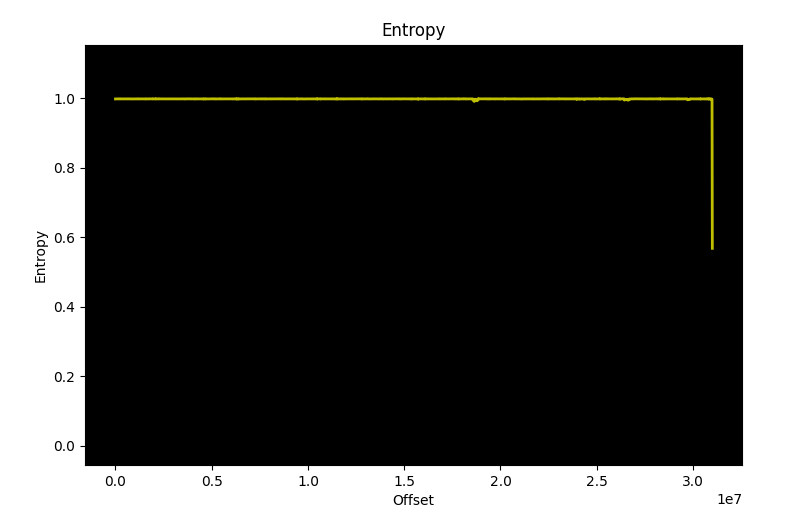
\includegraphics[scale=0.35]{r7000entropy.png}
    \caption{Gráfica de la entropía de la imagen firmware del Netgear R7000 generada por Binwalk.}
    \label{fig:binwalkEnt}
\end{figure}

\begin{figure}[H]
    \centering
    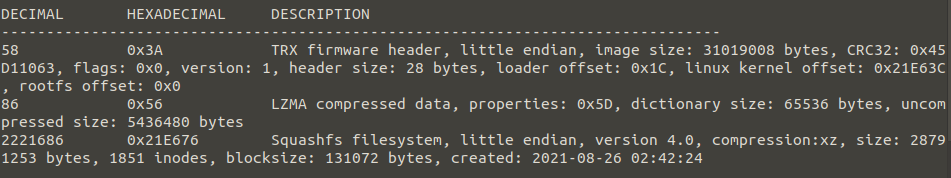
\includegraphics[scale=0.36]{r7000extraction.png}
    \caption{Extracción firmware Netgear R7000 usando Binwalk.}
    \label{fig:binwalkExt}
\end{figure}

\begin{figure}[H]
    \centering
    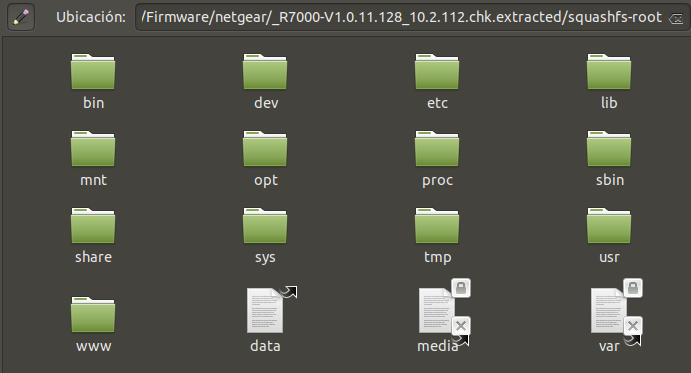
\includegraphics[scale=0.46]{r7000Squashfs.png}
    \caption{Sistema de archivos del Netgear R7000.}
    \label{fig:R7000squashfs}
\end{figure}

\begin{figure}[H]
    \centering
    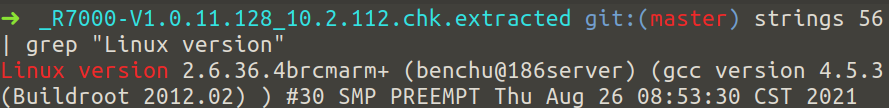
\includegraphics[scale=0.35]{r7000kernel.png}
    \caption{Versión del kernel utilizada por el R7000.}
    \label{fig:R7000kernel}
\end{figure}

Una vez extraído el firmware, podemos proceder a elegir un binario que nos resulte de interés para aplicarle fuzzing. Esto será
comentado en la siguiente sección.

\subsection{Introducción al experimento}
El experimento que va a ser llevado a cabo está basado en los descubrimientos realizados por el equipo de la firma de ciberseguridad GRIMM, publicados el
22 de Abril del 2022\cite{r7000GRIMM}. En su publicación, hacen una introducción a una vulnerabilidad detectada en el demonio UPNP presente en 
el firmware del Netgear R7000 en su versión 1.0.11.128 y anteriores. La vulnerabilidad se da concretamente en la funcionalidad de actualización de 
firmware proporcionada por el demonio UPNP y consiste en un desbordamiento de buffer que puede llevar a ejecución remota de código (RCE) por parte de un usuario 
identificado en el sistema al proporcionar un paquete de actualización de firmware malicioso. Esto es posible debido a que la rutina de actualización 
al comprobar los headers confía en los tamaños especificados en la cabecera TRX\cite{firmwareFormat} incluida en el paquete de firmware proporcionado 
por el usuario para realizar operaciones de memoria. A continuación, aplican emulación full-system en QEMU con el objetivo de recrear la vulnerabilidad 
y diseñar una prueba de concepto de un firmware malicioso.\bigskip

El equipo de GRIMM identificó la vulnerabilidad mediante análisis estático de código haciendo uso de herramientas de decompilación como Ghidra\cite{Ghidra}.
Aunque se trata de una técnica efectiva, requiere de un experto cualificado que revise manualmente el código línea a línea pudiendo potencialmente dar un veredicto incompleto. Como es lógico, no se trata de un procedimiento que pueda ser fácilmente escalable. Además, hacen uso de emulación full-system cuando solo desean
poner a prueba una pequeña parte de la funcionalidad del demonio. Es por ello que proponemos mejoras para ambos de los aspectos mencionados mediante la aplicación 
de técnicas alternativas. En primer lugar, respecto al procedimiento de identificación de la vulnerabilidad podemos hacer uso de fuzzing, realizando de forma 
automática mutaciones a la imagen del firmware que se proporciona a la rutina de actualización. Al aplicar fuzzing, posibilitamos la detección de vulnerabilidades 
similares a gran escala y ayudamos al revisor de código a evitar tener que analizar código superfluo pudiendo centrarse en analizar los crashes detectados por
el fuzzer, sabiendo ya que se trata de código problemático. En segundo lugar, podemos obtener una mejora de rendimiento sustituyendo la emulación full-system 
por el uso de técnicas basadas en Unicorn\cite{unicorn} que nos permitan instrumentar exactamente la rutina de actualización de firmware incluida en el 
demonio UPNP.\bigskip

En resumen, el objetivo del experimento es intentar identificar la misma vulnerabilidad pero haciéndolo a través de fuzzing, a la misma vez que comparamos el enfoque de 
emulación aplicado por el equipo de GRIMM con otras técnicas de emulación alternativas.

\subsection{Realización del experimento}
\subsubsection{Análisis del binario}
Comenzaremos por identificar el binario que implementa la funcionalidad del UPNP en el firmware y cargarlo en Ghidra\cite{Ghidra} para obtener una visión
decompilada o reconstruida del código original que nos permita encontrar la rutina de código que gestiona las actualizaciones del firmware. Para ello, 
accedemos al sistema de archivos que fue extraído del firmware previamente y abrimos con Ghidra el binario ubicado en ''usr/sbin/upnpd''. Una vez 
hecho esto, podemos guiar nuestra búsqueda por las cadenas de texto de mensajes de log presentes en el binario. Utilizando la funcionalidad de búsqueda 
de strings en Ghidra podemos buscar strings relacionadas con términos como ''firmware'', ''header'', ''update'' o similares. Dado que la vulnerabilidad 
se da a la hora de comprobar los headers del firmware, buscamos por ''header'' y rápidamente identificamos el string ''Header checksum error!!!'' 
siendo referenciado por dos funciones distintas (figura \ref{fig:R7000string}).

\begin{figure}[H]
    \centering
    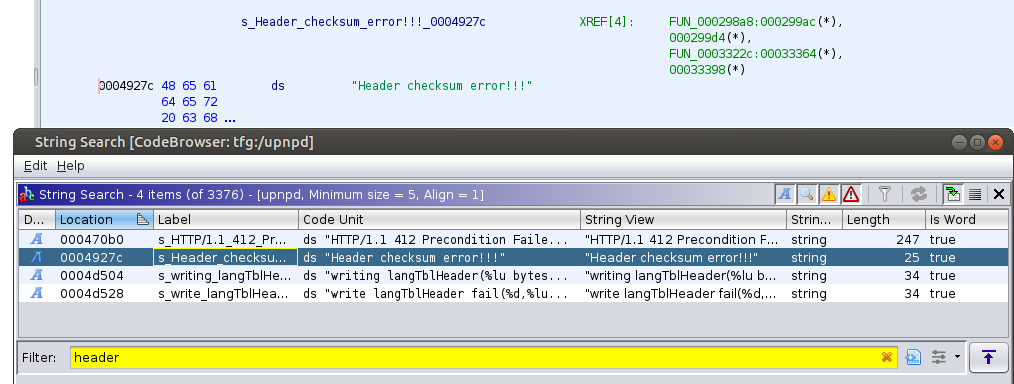
\includegraphics[scale=0.35]{r7000string.png}
    \caption{Resultados de la búsqueda de strings en Ghidra.}
    \label{fig:R7000string}
\end{figure}

Ambas funciones implementan aparentemente la misma lógica de parsing de la cabecera del firmware con la única diferencia de que ''FUN\_0003322c''
(figura \ref{fig:R7000decompilado}) contiene hardcodeado el modelo del dispositivo para compararlo con un valor incluido en el firmware. 
Ya que esta función parece destinada a nuestro modelo específico, será la función que usemos como objeto de pruebas más adelante y la apodaremos 
''check\_upd\_header'' a partir de ahora. Realizando un breve 
análisis del código decompilado, podemos observar que en la línea 17 se comprueba una cadena mágica para verificar que se trata de un firmware, 
en las líneas 29 y 30 se realizan operaciones con memoria que analizaremos más adelante y de la línea 34 a la 44 se llevan a cabo comprobaciones de que 
el firmware corresponda con el modelo de dispositivo en el que va a ser instalado.

\begin{figure}[H]
    \centering
    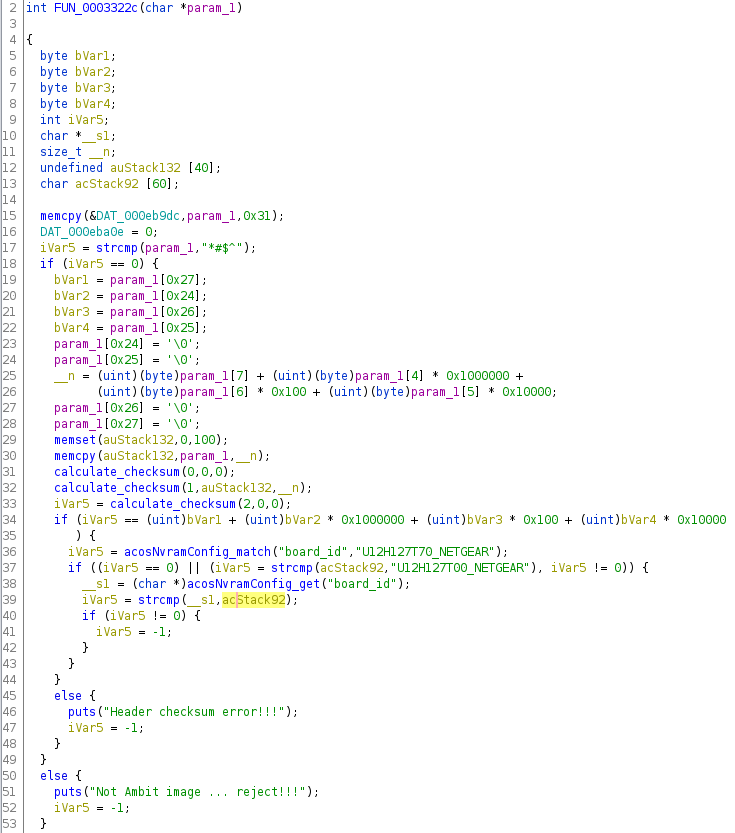
\includegraphics[scale=0.45]{r7000decompilado.png}
    \caption{Rutina de actualización de firmware decompilada por Ghidra.}
    \label{fig:R7000decompilado}
\end{figure}

\subsubsection{Emulación del binario}
Es imprescindible conseguir emular el binario como paso previo a aplicar fuzzing sin disponer del dispositivo original. Para ello, como se ha comentado 
anteriormente pondremos a prueba tanto la metodología de emulación QEMU full-system propuesta por GRIMM en su artículo como una emulación mediante 
Qiling\cite{qiling} que en lugar de emular el demonio en su totalidad, instrumente el binario para ejecutar exclusivamente la función que hemos identificado 
en la sección anterior. Además, pondremos a prueba la efectividad de FirmAE\cite{Kim2020} para comprobar si pudiera proporcionar una mejor experiencia de 
emulación full-system en comparación con QEMU básico.

\paragraph{Qiling}
Para emular la función deseada con Qiling, aplicaremos la misma técnica que ha sido desarrollada para instrumentar el código en la prueba de concepto anterior, es decir, se harán uso 
de dos hooks para alterar el flujo de ejecución del código. El primer hook se ejecutará al llegar al punto de entrada del ejecutable y reemplazará el primer 
parámetro de la función (registro R0 según la convención de llamada a funciones en ARM32) con la dirección en hexadecimal de check\_upd\_header() para convertir 
la función en el main del programa. El segundo hook también sigue el mismo funcionamiento, dado que check\_upd\_header() solo recibe como parámetro un array 
de bytes representando la cabecera del firmware, solo será necesario alocar manualmente los bytes que el script de Qiling haya leído de un archivo que se le 
pase por línea de comandos. En la figura \ref{fig:R7000flowchart} podemos observar el flujo de ejecución aplicando instrumentación 
dinámica con el script de Qiling.

\begin{figure}[H]
    \centering
    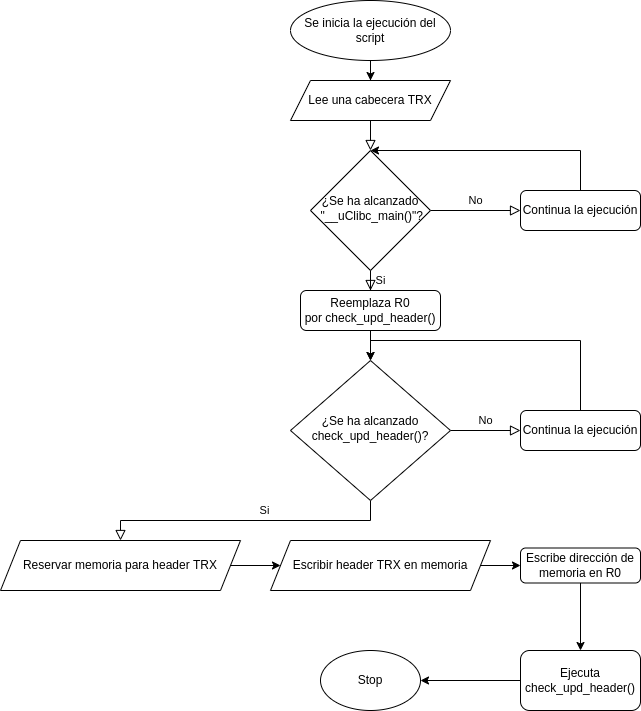
\includegraphics[scale=0.45]{r7000flowchart.png}
    \caption{Diagrama de flujo representando la instrumentación realizada sobre UPNP.}
    \label{fig:R7000flowchart}
\end{figure}

Para crear el script, empezamos consultando en Ghidra la dirección de la función ''\_\_uClibc\_main()'' y las direcciones de 
inicio y fin de la función objetivo check\_upd\_header() para crear variables reconocibles en el script. Para el caso de este 
binario, las direcciones son las siguientes:

\begin{lstlisting}[language=python, caption=Declaración de constantes: Direcciones de interés en funciones., captionpos=b,
     frame=single, breaklines]
    TARGET_FUNC_ADDR    = 0x3322c   # Address of the function we are interested in
    TARGET_END_ADDR     = 0x33360   # End fuzzing when reaching this address
    LIBC_START_ADDR     = 0x0c460   # Address where __uClibc_main is being called
\end{lstlisting}

Gracias a la intuitiva API de Qiling, establecer los hooks es tan fácil como asociar la dirección de una instrucción del binario
con una función del script. También cabe mencionar que definiremos como ''rootfs'' la ruta al sistema de archivos extraído del
firmware previamente para que el enlazado dinámico de librerías se produzca correctamente. Definimos de la siguiente manera los
hooks y sus callbacks asociados.

\begin{lstlisting}[language=python, caption=Definición de hooks del script de emulación para Qiling., captionpos=b,
    frame=single, breaklines]
    def libc_start_main_redirect(ql: Qiling, func_addr = TARGET_FUNC_ADDR):
    ql.reg.write("r0", func_addr)
    
    def indirect_write_reg_bytes(ql: Qiling, register_id, bytes):
        address = ql.mem.map_anywhere(len(bytes))
        ql.mem.write(address, bytes)
        ql.reg.write(register_id, address) # == (ql.reg.r0 = address) 

    def target_hook(ql: Qiling):    
        print("\n--------------\n")
        print("HOOK, PC: 0x%x" % ql.reg.arch_pc)
        print("Using", PAYLOAD, "as payload\n")
        indirect_write_reg_bytes(ql, "r0", PAYLOAD)
        print("\n--------------\n")
        
    def sandbox(path, rootfs, debug):    
        ql = Qiling(path, rootfs)
        ql.hook_address(libc_start_main_redirect, LIBC_START_ADDR)
        ql.hook_address(target_hook, TARGET_FUNC_ADDR)     
        ql.debugger = debug
        ql.run(end=TARGET_END_ADDR)

    ...
\end{lstlisting}

Tras crear el script, necesitaremos un ejemplo real de cabecera de firmware para pasarle a este como parámetro y comprobar así
su funcionamiento. Para ello, simularemos un caso de actualización de firmware real, es decir, descargaremos el paquete de 
firmware correspondiente a la siguiente versión (1.0.11.128 -> 1.0.11.134) y extraeremos los 1024 primeros bytes de este ya que 
solo estamos interesados en las cabeceras y el inicio del fichero. DD permite hacer esto con la siguiente orden:

\begin{lstlisting}[language=bash, breaklines]
    $ dd if=R7000-V1.0.11.134_10.2.119.chk of=header134.chk count=1 bs=1K
\end{lstlisting}

Mirando el volcado en hexadecimal del fichero resultante (figura \ref{fig:R7000header}), saltan rápidamente a la vista dos de
los campos descritos anteriormente al tratar la estructura de una cabecera TRX y las comprobaciones previas que realiza 
check\_upd\_header(), el magic number o cadena mágica al inicio del fichero con el valor ''*\#\$\textasciicircum'' y el modelo de dispositivo
para el que va destinada la actualización ''U12H270T00\_NETGEARHDR0''.

\begin{figure}[H]
    \centering
    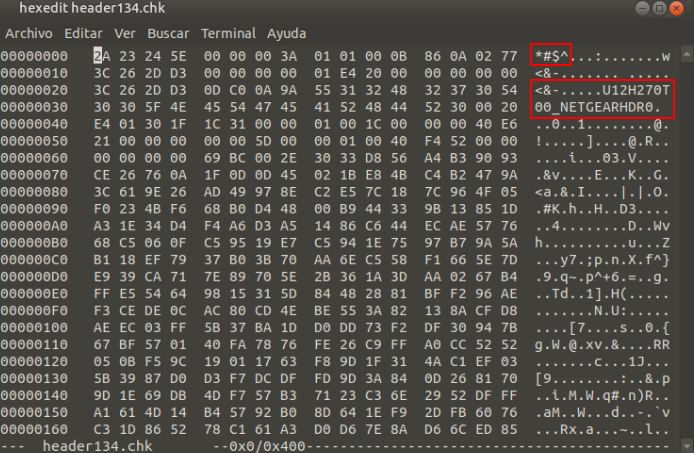
\includegraphics[scale=0.5]{r7000header.png}
    \caption{Representación hexadecimal del contenido del firmware.}
    \label{fig:R7000header}
\end{figure}

A continuación, podemos ejecutar el script y comprobar su funcionamiento. Al ejecutarlo pasando como parámetro 
''header134.chk'' (figura \ref{fig:R7000qiling}), observamos que los hooks se aplican correctamente y aunque la ejecución 
parece finalizar correctamente se muestran errores ENOENT debido a la ausencia de una NVRAM en ''/dev/nvram''. Esto se produce cuando la función emulada
intenta consultar en la NVRAM la variable ''board\_id'' para compararla con el string del modelo en el firmware comentado
anteriormente. Dado que no estamos emulando la NVRAM ni haciendo uso de librerías alternativas como nvram-faker\cite{nvram}
para interceptar las operaciones con este dispositivo, se producen errores al intentar consultar variables en este pero ya
que solo se utiliza para realizar la comparación de ambas cadenas, podemos ignorar los errores por el momento.

\begin{figure}[H]
    \centering
    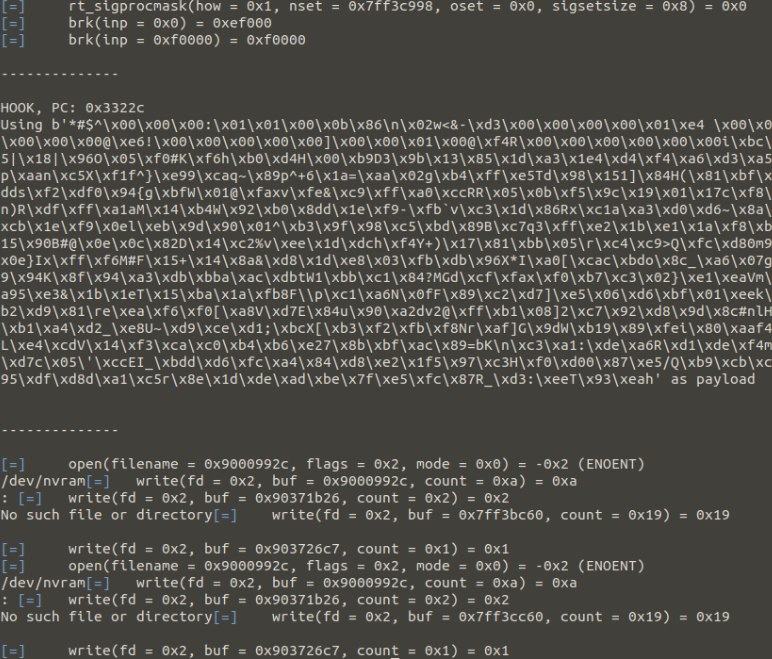
\includegraphics[scale=0.4]{r7000qiling.png}
    \caption{Resultado de la emulación de check\_upd\_header() con Qiling.}
    \label{fig:R7000qiling}
\end{figure}

Si probamos a modificar la cadena mágica del firmware y a pasárselo al script, comprobamos que efectivamente se avisa de que 
el fichero no se trata de una actualización de firmware válida (figura \ref{fig:R7000magic}), cancelando así el proceso de actualización si estuviéramos 
emulando el binario al completo.

\begin{figure}[H]
    \centering
    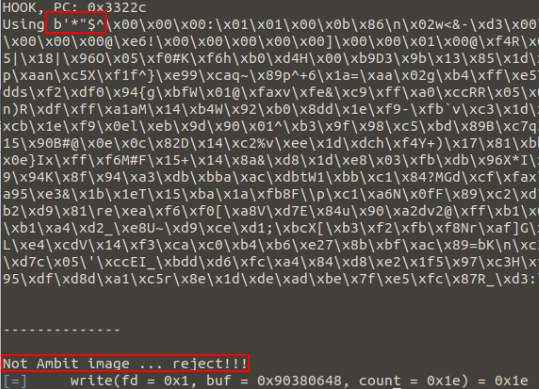
\includegraphics[scale=0.65]{r7000magic.png}
    \caption{Fallo al comprobar la cadena mágica en Qiling.}
    \label{fig:R7000magic}
\end{figure}

\paragraph{QEMU}
Para emular el firmware aplicando emulación full-system en QEMU, es más viable obtener una máquina virtual Linux para sistemas ARM 
y ejecutar en esta los binarios de interés antes que intentar emular el firmware del dispositivo al completo. Esto se debe a que para emular el firmware al completo sería necesario solucionar manualmente los problemas de compatibilidad que surgieran como diferencias en la configuración 
de interfaces red o la ausencia de dispositivos necesarios durante el arranque del sistema y su uso como hemos comprobado anteriormente 
con el NVRAM. Por ello, partimos de una VM de Debian ARM (debian-10-openstack-arm64.qcow2) obtenida de su  
\href{https://cdimage.debian.org/cdimage/cloud/OpenStack/}{web oficial} en la que introduciremos el sistema de archivos extraído del firmware 
del R7000 para ejecutar el binario del servicio UPNP teniendo todas las librerías necesarias para ello. Utilizamos la siguiente 
orden para arrancar la máquina virtual descargada con 2GB de RAM, todos los núcleos disponibles de la CPU, almacenamiento, un 
adaptador de red y los puertos 22 y 5000 redirigidos a la máquina host. El puerto 22 será de utilidad para acceder 
mediante SSH a la máquina virtual mientras que el 5000 lo necesitamos para poder realizar peticiones por el protocolo SOAP, el protocolo utilizado por el demonio UPNP para interactuar con este desde el exterior.

\begin{lstlisting}[language=bash, breaklines]
    $ qemu-system-aarch64 -m 2G -M virt -cpu max -bios /usr/share/qemu-efi-aarch64/QEMU_EFI.fd -drive if=none,file=debian-10-openstack-arm64.qcow2,id=hd0 -device virtio-blk-device,drive=hd0 -device e1000,netdev=net0 -netdev user,id=net0,hostfwd=tcp:127.0.0.1:1234-:22,hostfwd=tcp::5000-:5000 -nographic
\end{lstlisting}

\begin{figure}[H]
    \centering
    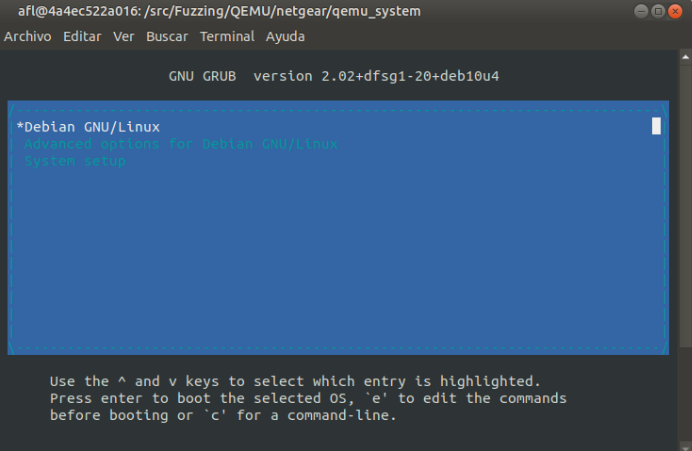
\includegraphics[scale=0.55]{r7000QemuBoot.png}
    \caption{Menú de la GRUB en la VM Debian ARM para QEMU.}
    \label{fig:R7000QemuBoot}
\end{figure}

Al finalizar el arranque de la máquina virtual, podemos utilizar \textit{chroot} para cambiar el directorio raíz actual al directorio 
del sistema de archivos extraído del router previamente (figura \ref{fig:R7000shell}). Desafortunadamente, al poner en marcha el 
servicio del UPNP comprobamos que no es capaz de funcionar correctamente en el entorno virtual actual. Como documenta GRIMM\cite{r7000GRIMM}
en sus descubrimientos, esto se debe a una mala configuración de las interfaces red y a la falta de una NVRAM desde la que leer los 
parámetros de configuración del servicio. Este tipo de problemas son de esperar al aplicar técnicas de emulación full-system y han 
de ser solventados para conseguir que el demonio se ejecute correctamente.

\begin{figure}[H]
    \centering
    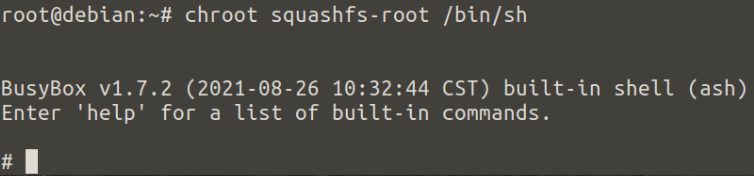
\includegraphics[scale=0.55]{r7000shell.png}
    \caption{Busybox shell desde el sistema de archivos del R7000.}
    \label{fig:R7000shell}
\end{figure}

Para solucionar estos problemas haremos uso de las soluciones proporcionadas por el equipo de GRIMM\cite{r7000GRIMM}. En primer
lugar, modificaremos el flujo de ejecución del binario con GDB para evitar llamar a \textit{exit()} al fallar el bloque de código 
que realizar la comprobación de las interfaces de red. Como podemos ver en la versión decompilada del código que realiza dicha 
comprobación mostrada en la figura \ref{fig:R7000iffix}, será necesario establecer un breakpoint al llegar a ''FUN\_0000e4c8''
para que cuando esto suceda, cambiar el contador de programa a la dirección del return de la función con el objetivo de saltarnos 
la comprobación. Para solucionar la falta de una NVRAM, reemplazaremos la librería dinámica ''libnvram.so'' del sistema de archivos 
por una versión modificada de nvram-faker\cite{nvram} que GRIMM proporciona con las variables extraídas de un dispositivo original.
Esto resulta un claro punto negativo para la aplicación de emulación full-system, ya que para conseguir que nuestro binario de 
interés se ejecute correctamente, hubiéramos necesitado disponer del dispositivo original para identificar todas las variables 
consultadas en la NVRAM y volcar sus valores esperados a través de ingeniería inversa.

\begin{figure}[H]
    \centering
    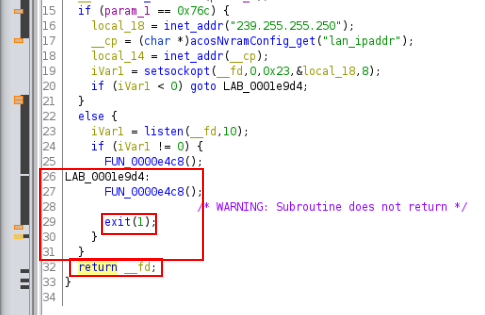
\includegraphics[scale=0.65]{r7000iffix.png}
    \caption{Rutina de comprobación de interfaces de red R7000.}
    \label{fig:R7000iffix}
\end{figure}

Tras solucionar los problemas encontrados, hacemos uso de la siguiente orden para automatizar el proceso de hacer \textit{chroot}
al sistema de archivos, ejecutar UPNP en segundo plano, attachear GDB a este proceso y llevar a cabo el cambio de flujo descrito mediante un script de GDB.
Esta vez, ya es posible realizar peticiones por el puerto 5000 al servicio a través de CURL (figura \ref{fig:R7000QemuWorking}). Por ahora nos sirve 
con saber que el servicio está operativo y es capaz de responder peticiones pero más adelante, crearemos un script para llevar a cabo las peticiones 
SOAP necesarias a través de HTTP para iniciar la funcionalidad de actualización de firmware.

\begin{lstlisting}[language=bash, breaklines]
    $ chroot squashfs-root /bin/sh -c "/usr/sbin/upnpd&" && gdb -x ./gdb_script -q -p `pgrep upnpd`
\end{lstlisting}

\begin{figure}[H]
    \centering
    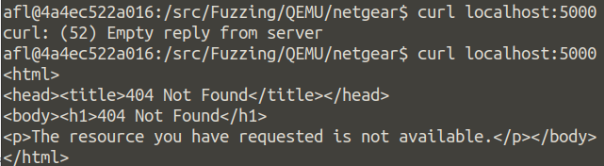
\includegraphics[scale=0.65]{r7000QemuWorking.png}
    \caption{UPNP respondiendo una petición GET básica.}
    \label{fig:R7000QemuWorking}
\end{figure}

\paragraph{FirmAE}
Como se comentó en el apartado ''\nameref{estado_del_arte}'', FirmAE fue desarrollado con el objetivo de poder solucionar mediante heurísticas 
pequeños problemas de configuración como los que hemos experimentado al intentar emular el binario con QEMU básico. Por ello, 
procederemos a poner esta herramienta en práctica para comprobar si emular el firmware en su totalidad con esta herramienta supone alguna mejoría con respecto a la metodología seguida
por GRIMM\cite{r7000GRIMM}.

Iniciar la emulación del firmware con FirmAE es tan simple como indicarle la ruta a la imagen firmware del dispositivo. A continuación, 
FirmAE extrae y analiza dinámicamente el firmware durante aproximadamente diez minutos para intentar detectar problemas de configuración y 
ajustar el entorno de emulación con el objetivo de satisfacer sus necesidades (figura \ref{fig:R7000FirmAE}). 

\begin{figure}[H]
    \centering
    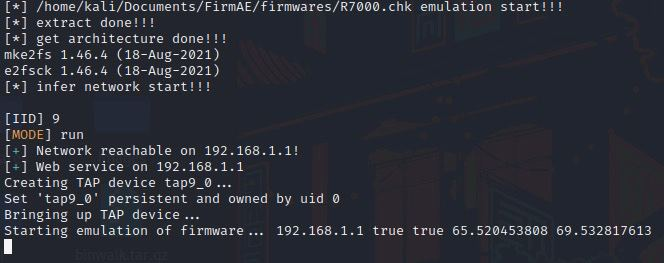
\includegraphics[scale=0.54]{r7000FirmAE.png}
    \caption{Instancia de FirmAE emulando el firmware de un R7000.}
    \label{fig:R7000FirmAE}
\end{figure}

Al intentar acceder a la dirección IP local que ha habilitado FirmAE para el portal web del dispositivo, nos encontramos con el proceso de 
configuración original de Netgear (figura \ref{fig:R7000Setup}) el cual no podemos completar porque el resto del proceso de configuración se lleva a cabo
en la dirección ''www.routerlogin.net'' y el firmware asume que se está utilizando el servidor DNS del router emulado, por lo que no se nos redirige 
correctamente a la configuración al visitar dicha dirección. Esto puede solucionarse editando el fichero ''/etc/hosts'' en Linux para que 
el hostname ''routerlogin.net'' resuelva a la dirección IP asignada por FirmAE. Tras este cambio somos capaces de finalizar la configuración inicial 
y de acceder al panel de control del router (figura \ref{fig:R7000panel}). 

\begin{figure}[H]
    \centering
    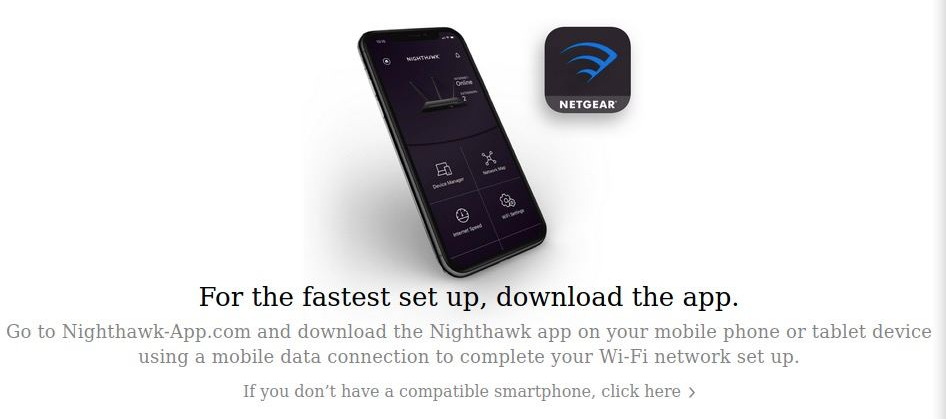
\includegraphics[scale=0.5]{r7000Setup.png}
    \caption{Setup de configuración del R7000.}
    \label{fig:R7000Setup}
\end{figure}

\begin{figure}[H]
    \centering
    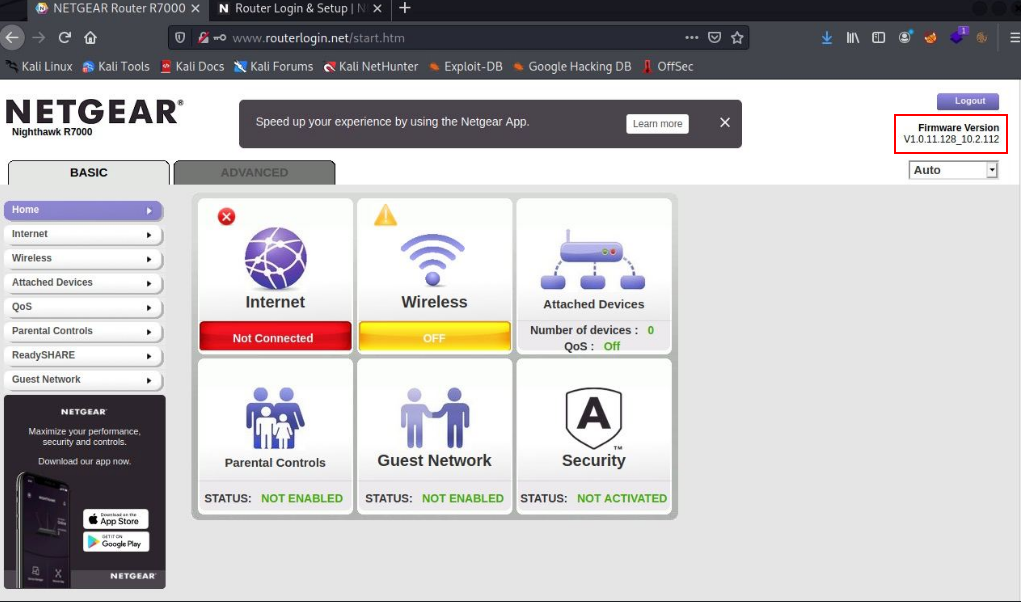
\includegraphics[scale=0.45]{r7000panel.png}
    \caption{Panel de control del R7000.}
    \label{fig:R7000panel}
\end{figure}

Por desgracia, aunque el portal web principal parece estar siendo correctamente emulado, solo obtenemos ''empty response'' al realizar peticiones
por el puerto 5000 al demonio UPNP. Ejecutando manualmente el binario desde la shell proporcionada por FirmAE, observamos que la ejecución 
entra en un bucle infinito intentando llevar a cabo operaciones en exclusión mutua relacionadas con el uso de variables de la NVRAM 
(figura \ref{fig:R7000FirmAEupnp}). Dado que el problema sigue presente incluso al usar nvram-faker\cite{nvram} de la misma forma que se ha aplicado anteriormente para QEMU básico, la emulación del firmware
a través de FirmAE queda descartada.

\begin{figure}[H]
    \centering
    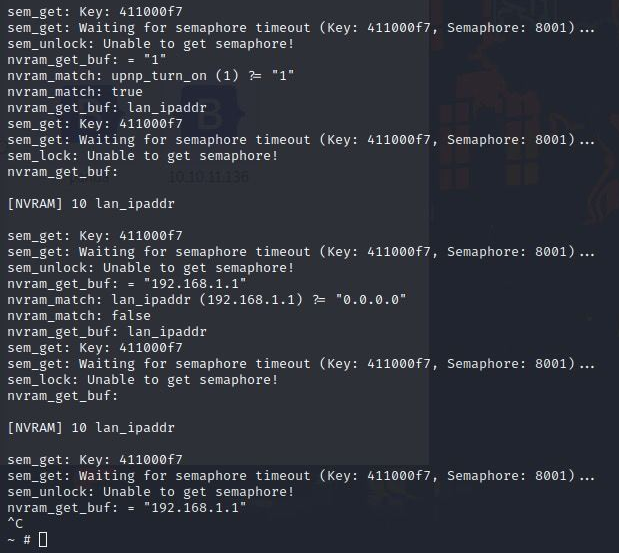
\includegraphics[scale=0.5]{r7000FirmAEupnp.png}
    \caption{Bucle infinito al ejecutar UPNP con FirmAE.}
    \label{fig:R7000FirmAEupnp}
\end{figure}

\subsubsection{Aplicación de fuzzing}
Tras conseguir emular el servicio UPNP del firmware aplicando tanto emulación full-system en QEMU como emulación basada en Unicorn\cite{unicorn}
con Qiling\cite{qiling}, procederemos a aplicar fuzzing sobre dicho servicio con el objetivo de explorar otras técnicas a partir de las cuales 
se podría haber llegado a esta vulnerabilidad además de compararlas entre sí.

\paragraph{Vulnerabilidad a identificar} Como se ha comentado en la introducción al experimento, buscamos alcanzar a través de fuzzing una 
vulnerabilidad previamente conocida y gracias a que partimos sabiendo qué se trata buscar, procederemos a analizar brevemente dicha vulnerabilidad
sobre el código decompilado (figura \ref{fig:UpnpCheckHeader}) con el objetivo de facilitar al lector la comprensión del experimento, los problemas encontrados y los resultados de este. 
El funcionamiento de ''check\_upd\_header()'' puede dividirse en cinco pasos principales. En primer lugar, se comprueba que el firmware tenga 
la cadena mágica ''*\#\$\textasciicircum'' al inicio mediante una llamada a la función \textit{strcmp} sobre el array de bytes que representa al 
firmware. Esto es posible debido a que las cadenas de caracteres en C vienen delimitadas por un byte nulo al final y recordemos que los campos de 
las cabeceras TRX\cite{firmwareFormat} vienen también delimitadas por bytes nulos. En el segundo paso se utiliza la siguiente 
sección de la cabecera para consultar el tamaño de esta. El principal problema de este paso y el factor que causa la vulnerabilidad que estamos tratando
es la ausencia de validación de los datos que están siendo recibidos del exterior los cuales nunca deberían de ser confiados, aún menos cuando van a ser utilizado como parámetro en operaciones con memoria a continuación en el tercer paso. Dado que el usuario desde el exterior
puede fijar cuantos bytes van a ser copiados sobre el buffer de destino, este podría provocar un desbordamiento de la pila, pudiendo también modificar la 
dirección de retorno de la función además de diversos registros usados para almacenar variables locales en ARM32 (R4-R11). Por último, en los pasos 
cuatro y cinco se llevan a cabo comprobaciones adicionales sobre el checksum y el modelo del dispositivo para evitar que el usuario aplique un paquete
de firmware incorrecto o corrupto.

Para que un fuzzer sea capaz de identificar el crash producido por el desbordamiento de la pila, este tendrá que generar un input mutado que respete la 
cadena mágica inicial además de incluir en el campo del tamaño de la cabecera un valor superior al admitido por el buffer de destino ubicado en la pila.

\begin{figure}[H]
    \centering
    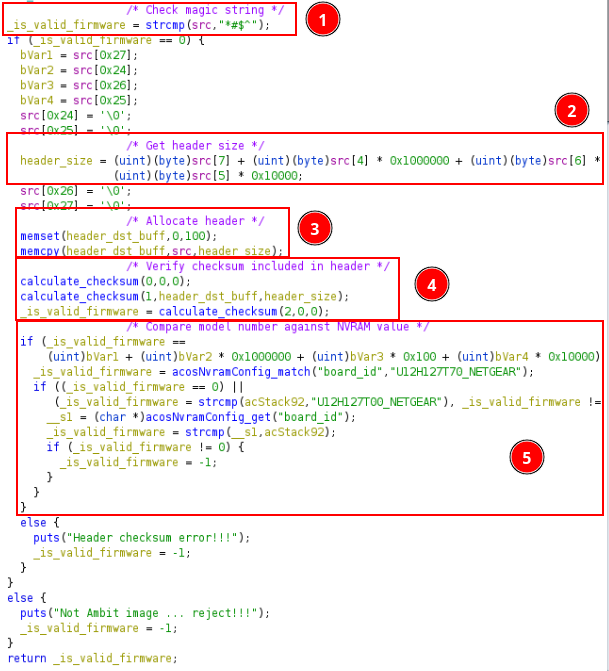
\includegraphics[scale=0.55]{UpnpCheckHeader.png}
    \caption{Decompilado de la función ''check\_upd\_header()'' comentado.}
    \label{fig:UpnpCheckHeader}
\end{figure}

\paragraph{Fuzzing con Qiling}
Para realizar fuzzing usando Qiling, partimos del script que ha sido desarrollado previamente para la emulación e instrumentación del binario al
cual se le realizarán algunas modificaciones para integrar la lectura de inputs con un fuzzer de caja gris como es AFL++\cite{afl++}. Además, también se 
creará una versión del script que utilice a Radamsa\cite{radamsa} como generador de inputs para poder comprobar si un fuzzer de caja negra
pudiera dar mejores resultados que uno de caja gris en determinadas situaciones.\bigskip

Empezando por integrar el script de Qiling con AFL++, haremos uso de los bindings para Python que proporciona AFL++ como parte de su integración
con Unicorn (Unicornafl). El flujo de ejecución será el mismo, con la diferencia de que el almacenamiento de los bytes de la cabecera en memoria se hará ahora 
dentro de un callback que será llamado por AFL++ cada vez que este desee realizar una nueva iteración durante el fuzzing. De esta forma hacemos
uso de dos hooks, un primer hook que lleva a cabo el cambio del punto de entrada del binario de la misma manera que en el script de emulación y un 
segundo que llama a una función encargada de reportar a AFL++ que se ha llegado al punto de inicio para el fuzzing. Por último, adelantamos la 
dirección en la que finaliza la ejecución del binario modificando ''TARGET\_END\_ADDR'' para evitar realizar las comparaciones del modelo del 
dispositivo, ya que de todas formas no estaban siendo emuladas correctamente al carecer de una NVRAM. Tener que emular un menor número de 
instrucciones por ejecución del script supone una mejora en el número de ejecuciones por segundo. El script resultante es el siguiente donde 
''place\_input\_callback()'' es la función llamada por AFL++ para almacenar los inputs mutados en memoria y ''start\_afl()'' la función a ejecutar 
al llegar ''check\_upd\_header()'' para comenzar una nueva iteración de fuzzing.

\begin{lstlisting}[language=python, caption=Script de fuzzing de UPNP para Qiling., captionpos=b,
    frame=single, breaklines, showstringspaces=false]
    import sys, os
    from qiling import Qiling
    from qiling.extensions.afl import ql_afl_fuzz
    
    TARGET_FUNC_ADDR    = 0x3322c   # Address of the function we are interested in
    TARGET_END_ADDR     = 0x3330c   # End fuzzing when reaching this address
    LIBC_START_ADDR     = 0x0c460   # Address where __libc_start_main is being called
        
    def libc_start_main_redirect(ql: Qiling, func_addr = TARGET_FUNC_ADDR):
        ql.arch.regs.write("r0", func_addr)
        
    def sandbox(path, rootfs, debug, param_file):
        ql = Qiling(path, rootfs)
        ql.hook_address(libc_start_main_redirect, LIBC_START_ADDR)
        
        def place_input_callback(_ql: Qiling, input: bytes, _):
            address = _ql.mem.map_anywhere(len(input))
            
            print("\n\n FILE LENGTH (bytes): ", len(input))
            
            _ql.mem.write(address, input)
            _ql.arch.regs.write("r0", address)
            
            res = _ql.mem.read(address, len(input));
            print("\n\n FUNCTION INPUT BYTES: \n\n", input)
            print("\n\n BYTES STORED IN MEMORY: \n\n", res)
            
        def start_afl(_ql: Qiling):
            ql_afl_fuzz(_ql, param_file, place_input_callback, exits=[ql.os.exit_point])
        
        ql.hook_address(start_afl, TARGET_FUNC_ADDR)
    
        try:
            ql.run()
            os._exit(0)
        except:
            os._exit(1)
        
        ...
\end{lstlisting}

Gracias a nuestro script, podemos iniciar una sesión de fuzzing en AFL++ (figura \ref{fig:R7000QilingFuzz}) con la siguiente orden, donde ''fuzz\_setup/in''
es un directorio que contiene un corpus formado por los primeros 1024 bytes de las dos imágenes del firmware en sus versiones 1.0.11.128 y 1.0.11.134,
mientras que ''fuzz\_setup/out'' será el directorio donde AFL++ almacene los resultados de la sesión de fuzzing (crashes o timeouts identificados, estadísticas de 
la sesión\dots). Además, con el objetivo de reducir el número de inputs que son descartados prematuramente en la comprobación de la cadena mágica, 
hacemos uso de la funcionalidad de diccionarios de AFL++ (flag -x) con un diccionario que contenga la cadena ''*\#\$\textasciicircum''.
\begin{lstlisting}[language=bash, breaklines]
    $ afl-fuzz -i fuzz_setup/in -o fuzz_setup/out -x dict/dictionary -U -- python3 ./src/dev/fuzz.py @@
\end{lstlisting}

Viendo que el fuzzing se realiza correctamente y que se descubren nuevos caminos a explorar en el código (la variable ''last new find'' se reinicia frecuentemente en AFL++), procedemos a dejar la 
sesión de fuzzing corriendo hasta que llegue al punto en el que AFL++ no detecte nuevos sucesos durante el fuzzing. AFL++ indica cuándo
esto sucede a través del color de la variable ''cycles done'', la cual cambia a color verde cuando no se ha alcanzado nuevo código 
ni se han visto diferencias en el comportamiento de este durante un tiempo. En este caso, el tiempo que se dedicó al proceso de fuzzing 
fue un total de 20 horas y 31 minutos corriendo en modo paralelo con 3 instancias del fuzzer simultáneas (\ref{fig:R7000parallel}).

\begin{figure}[H]
    \centering
    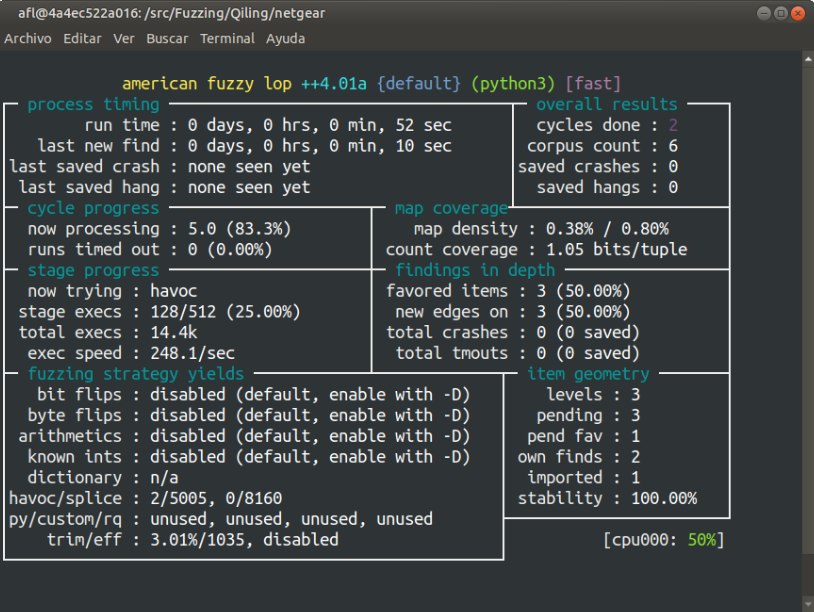
\includegraphics[scale=0.5]{r7000QilingFuzz.png}
    \caption{Sesión de fuzzing sobre UPNP usando Qiling.}
    \label{fig:R7000QilingFuzz}
\end{figure}

\begin{figure}[H]
    \centering
    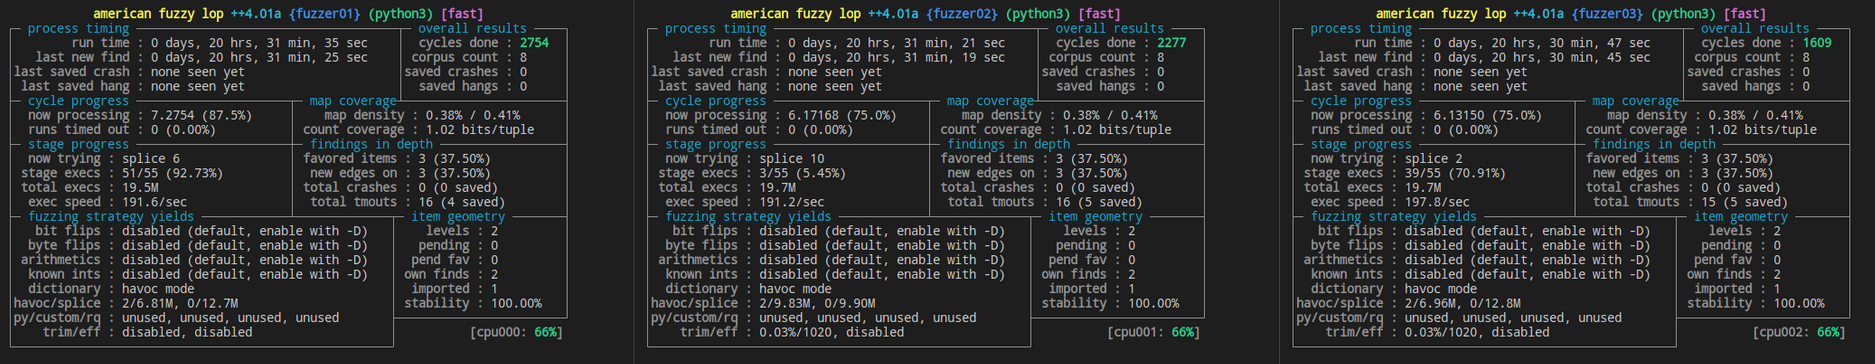
\includegraphics[scale=0.25]{AFLparallel.png}
    \caption{Sesión de fuzzing sobre UPNP con tres instancias en paralelo.}
    \label{fig:R7000parallel}
\end{figure}

\paragraph{Fuzzing con QEMU full-system}
Para este caso desarrollaremos un script en Python que nos permita llevar a cabo repetidas peticiones HTTP
al servicio UPNP mutando exclusivamente el firmware enviado. Para el aspecto de la generación de
inputs utilizaremos el fuzzer de caja negra Radamsa\cite{radamsa} debido a su excelente algoritmo 
de mutación además de estar diseñado para ser fácilmente integrable con scripts. Este experimento nos 
permitirá comprobar si la información adicional de feedback utilizada en el fuzzing de caja gris es 
de utilidad para este caso en comparación con el fuzzing de caja negra.\bigskip

El script a desarrollar deberá de en primer lugar, iniciar sesión en el servicio UPNP para obtener una cookie de sesión
previamente a mutar el firmware y enviarlo. Ya que UPNP trabaja en este caso mediante el protocolo SOAP a través de HTTP,
tendremos que realizar peticiones que sigan el formato correspondiente como podemos observar en la figura \ref{fig:SOAPlogin}
para la obtención de la cookie de sesión y en la figura \ref{fig:SOAPupdate} para iniciar la actualización de firmware.
Ambas peticiones serán tratadas más en profundidad a continuación con el desarrollo del script.

\begin{figure}[H]
    \centering
    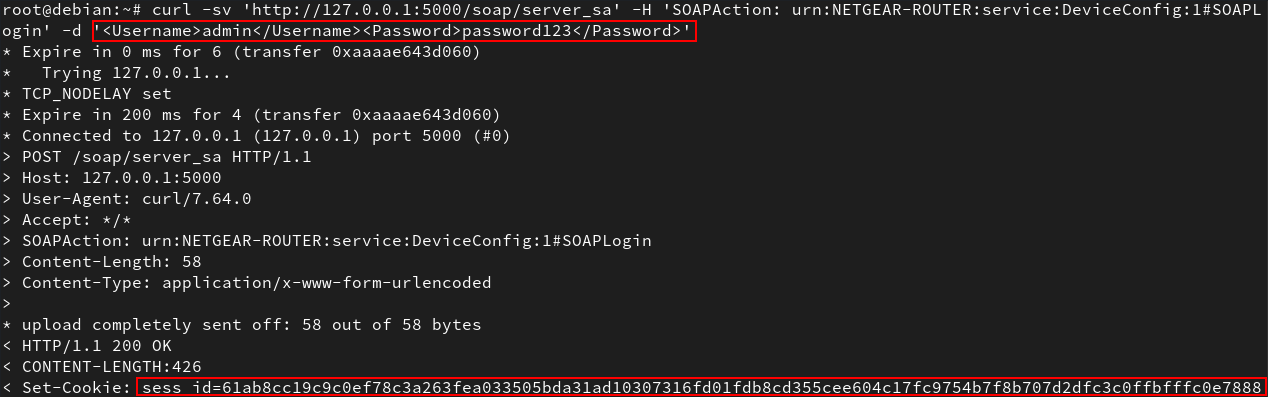
\includegraphics[scale=0.35]{SOAPlogin.png}
    \caption{Petición de login al servicio UPNP.}
    \label{fig:SOAPlogin}
\end{figure}

\begin{figure}[H]
    \centering
    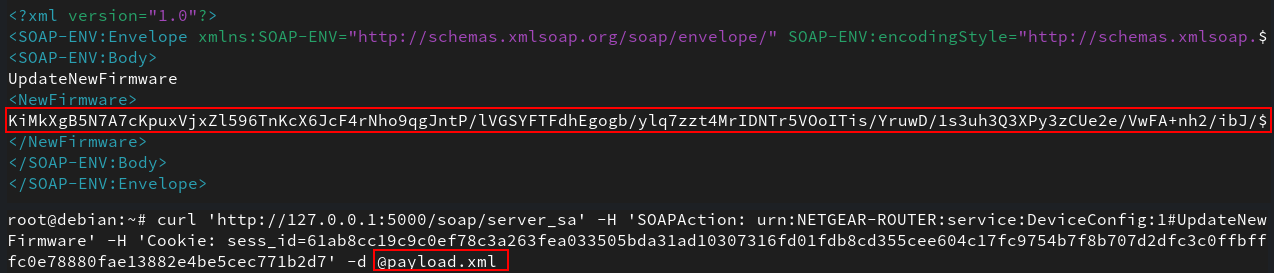
\includegraphics[scale=0.35]{SOAPupdate.png}
    \caption{Petición de actualización de firmware al servicio UPNP.}
    \label{fig:SOAPupdate}
\end{figure}

La función ''login()'' de nuestro script enviará una petición HTTP al endpoint 
''http://127.0.0.1:5000/soap/server\_sa'', indicando en la cabecera que la acción SOAP a realizar es ''SOAPLogin''
e incluyendo en los datos de la petición el usuario y contraseña por defecto del administrador. Una vez 
recibida la respuesta, extraemos el valor de la cookie ''sess\_id'' para realizar posteriormente peticiones
autenticadas.

\begin{lstlisting}[language=python, caption=Función para realizar login en el servicio UPNP., captionpos=b,
    frame=single, breaklines, showstringspaces=false]
    def login():
        url = 'http://127.0.0.1:5000/soap/server_sa'
        header = {'SOAPAction': 'urn:NETGEAR-ROUTER:service:DeviceConfig:1#SOAPLogin'}
        data = '<Username>admin</Username><Password>password123</Password>'
        
        response = requests.post(url, headers=header, data=data)
        cookie = response.cookies.get_dict()["sess_id"]
        return cookie
\end{lstlisting}

La función ''sendUpdate()'' iniciará el proceso de actualización de firmware mandando la petición correspondiente al 
UPNP. Para ello, se enviará otra petición al mismo endpoint ahora con la acción SOAP ''UpdateNewFirmware'' en el header,
incluyendo la cookie de sesión obtenida por la función ''login()'', además del firmware codificado en base64 como parámetro 
de la petición dentro de un XML. Dado el enfoque de caja negra que estamos aplicando en este caso, la forma en la que comprobamos 
si la petición realizada ha producido algún efecto adverso en el servicio es realizando un liveness-check con la función ''crashTest()''
cuando el servicio no ha respondido correctamente nuestra petición de actualización de firmware. De esta forma, si se produce algún error
en la conexión, se realizará una simple petición HTTP al servicio UPNP para verificar si este sigue operativo. En caso de fallar la 
verificación asumimos que se ha producido un crash, registramos el timestamp y almacenamos el input mutado que lo ha generado con la función
''dumpCrash()''.

\begin{lstlisting}[language=python, caption=Envío de actualización de firmware al servicio UPNP., captionpos=b,
    frame=single, breaklines, showstringspaces=false]
    def sendUpdate(loginCookie, xml):
        timeout = 10
        url = 'http://127.0.0.1:5000/soap/server_sa'
        header = {'SOAPAction': 'urn:NETGEAR-ROUTER:service:DeviceConfig:1#UpdateNewFirmware'}
        cookie = {'sess_id': loginCookie}
        data = xml
        
        try:
            response = requests.post(url, data=data, headers=header, cookies=cookie, timeout=timeout)
            print(response.text)
        except requests.exceptions.ConnectionError:
            print("Connection aborted :(\n")
            if (crashTest()):
                dumpCrash(xml)
                
        except requests.exceptions.ReadTimeout:
            dumpCrash(xml)

    def crashTest():
        url = 'http://127.0.0.1:5000/soap/server_sa'
        try:
            requests.get(url)
            return False
        except:
            return True

    def dumpCrash(xml):
        print("\nFOUND POTENTIAL CRASH\n")
        ts = datetime.datetime.now().strftime("%m-%d-%Y_%H:%M:%S") + ".dmp"
        print("Saving dump at ./"+ts)
        f = open(ts, "w+")
        f.write(xml)
        f.close()
        exit(1)
\end{lstlisting}

Respecto a la generación del XML, la API SOAP requiere que los datos incluidos como parte de la petición han de estar estructurados 
dentro de un SOAP Envelope. Concretamente, necesitaremos incluir el firmware dentro del cuerpo del envelope indicando también en este 
la acción de ''UpdateNewFirmware''. Esta funcionalidad queda implementada en la función ''craftXML()''.

\begin{lstlisting}[language=python, caption=Generación del XML envelope con el firmware para la actualización desde UPNP., captionpos=b,
    frame=single, breaklines, showstringspaces=false]
    def craftXML(payload):
        xml = '<?xml version="1.0"?>\r\n'
        xml += '<SOAP-ENV:Envelope xmlns:SOAP-ENV="http://schemas.xmlsoap.org/soap/envelope/" SOAP-ENV:encodingStyle="http://schemas.xmlsoap.$\r\n'
        xml += '<SOAP-ENV:Body>\r\n'
        xml += 'UpdateNewFirmware\r\n'
        xml += '<NewFirmware>\r\n'
        xml += base64.b64encode(payload).decode("utf-8")
        xml += '\r\n</NewFirmware>\r\n'
        xml += '</SOAP-ENV:Body>\r\n'
        xml += '</SOAP-ENV:Envelope>\r\n'
        
        return xml
\end{lstlisting}

Por último, debemos gestionar la mutación del firmware para poder llevar a cabo el proceso de fuzzing. Radamsa realiza las 
mutaciones a partir de una semilla y de un primer input que utilizará como punto de partida. La semilla es un valor numérico 
que puede ser aleatorio o fijado manualmente si se desea que se generen mutaciones deterministas, por lo que ofreceremos en 
el script la posibilidad de fijar un valor inicial para la semilla el cual irá siendo incrementado. En resumen, se invocará
a Radamsa dentro de un bucle infinito utilizando la imagen firmware versión 1.0.11.134 como punto de partida y se utilizará 
el output generado en cada iteración para realizar una petición de actualización de firmware al servicio UPNP, intentando 
detectar si alguna de las peticiones realizadas consigue afectar al correcto funcionamiento del servicio.

\begin{lstlisting}[language=python, caption=Integración con Radamsa para mutación de inputs., captionpos=b,
    frame=single, breaklines, showstringspaces=false]
    while(True):
        command = 'radamsa '
        
        if seed:
            command += '--seed ' + "% s" % seed + ' '
            seed += 1
        
        payload = subprocess.check_output(command + firmware_path, shell=True)
        xml = craftXML(payload)
        sendUpdate(cookie, xml)
\end{lstlisting}

Con el script completado y el servicio UPNP corriendo en la máquina virtual de QEMU, solo queda ejecutar el script para 
comenzar la sesión de fuzzing. En la figura \ref{fig:SOAPfuzzing} vemos como desde el script se van recibiendo las respuestas a las peticiones 
realizadas al servicio mientras que en la figura \ref{fig:SOAPprocessing} podemos ver los mensajes generados internamente por
UPNP al procesar las peticiones.

\begin{figure}[H]
    \centering
    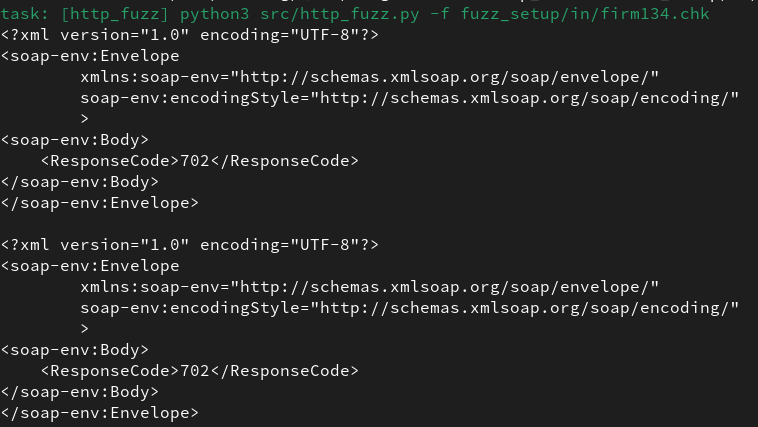
\includegraphics[scale=0.6]{SOAPfuzzing.png}
    \caption{Funcionamiento del script de fuzzing HTTP a UPNP.}
    \label{fig:SOAPfuzzing}
\end{figure}

\begin{figure}[H]
    \centering
    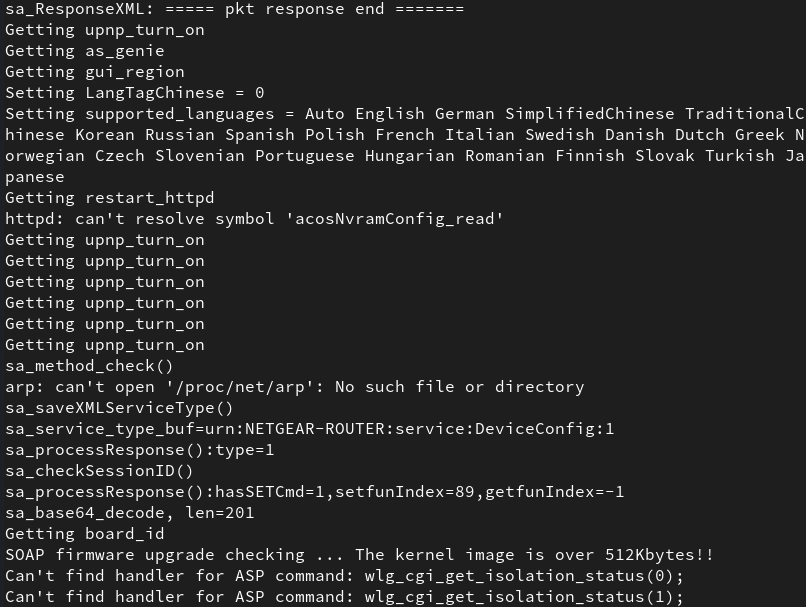
\includegraphics[scale=0.5]{SOAPprocessing.png}
    \caption{Servicio UPNP emulado procesando peticiones.}
    \label{fig:SOAPprocessing}
\end{figure}

\subsection{Resultados}
\subsubsection{Fuzzing con Qiling y AFL++}
Usar un script de Qiling con los bindings de python de Unicornafl para la integración con AFL++ ha resultado ser la opción menos efectiva. 
Aunque la parte de emulación se llevaba a cabo correctamente y con un gran incremento de velocidad gracias a tener que emular solo una función de 
código, tras las veinte horas y media de fuzzing no se detectó un solo crash ni timeout. Para analizar lo que estaba sucediendo, podemos hacer 
uso de la variable de entorno ''AFL\_DEBUG\_CHILD'' para ver el output del script en cada iteración de fuzzing. Haciendo esto, se detectaron dos 
problemas en la sesión de fuzzing causados por el mismo problema, uno a la hora de parsear los inputs del corpus y otro a la hora de mutarlos.\bigskip

Analizando el output de debugging se descubrió que Unicornafl, el componente de AFL++ que 
aporta la integración con Unicorn (y consecuentemente, Qiling) no gestiona correctamente los inputs que utilizan bytes nulos intercalados 
entre el resto de bytes. Esto provoca que por ejemplo, para las cabeceras de firmware que utilizamos como parte del corpus sus bytes sean 
tratados como una string de C y no como bytes, es decir, que a partir del primer byte nulo, el resto de bytes a continuación sean ignorados 
(figura \ref{fig:QilingDebug}). De esta forma, cuando AFL++ recibe un input para mutarlo, solo recibe los bytes de la primera sección 
de la cabecera TRX (la cadena mágica) y no es capaz 
de respetar la separación entre los campos de la cabecera mediante bytes nulos. Esto explica por qué no se ha obtenido ningún crash, ya que 
nunca se ha dado el caso de haber generado un input con la cadena mágica correcta delimitada por un byte nulo que además tuviera una valor 
excesivo en el siguiente campo del header para la longitud de este. Este problema ha sido discutido y reconocido por los principales 
desarrolladores del proyecto a través de Telegram y se ha dejado constancia a mediante la creación de un reporte a modo de issue en su repositorio
de \href{https://github.com/AFLplusplus/unicornafl/issues/13}{Github}. 
\begin{figure}[H]
    \centering
    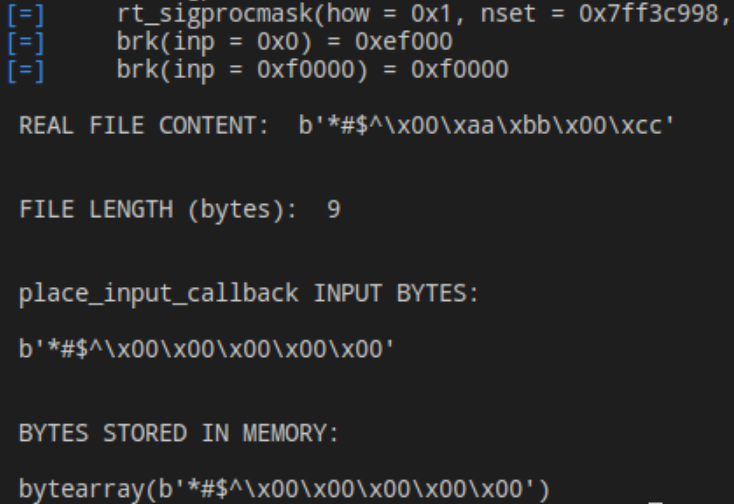
\includegraphics[scale=0.5]{QilingDebug.png}
    \caption{Mensajes de depuración en el script de Qiling mostrando la incorrecta gestión de inputs.}
    \label{fig:QilingDebug}
\end{figure}

Como solución temporal, podemos manualmente en el script de Qiling modificar el callback que almacena los inputs en memoria para fijar a 0
los bytes que actúen como delimitadores de las distintas secciones de una cabecera TRX. Por ejemplo, solo fijando a 0 el byte cuarto del input
(el que delimita la cadena mágica) ya podemos ver crashes en AFL++ en alrededor de un minuto (figura \ref{fig:QilingCheat}). Al analizar uno 
de los crashes generados (\ref{fig:UPNPQilingCrash}) apreciamos que efectivamente, AFL++ no ha introducido bytes nulos en el input para
separar las secciones y que si ha crasheado, ha sido por introducirlos manualmente desde el script previamente a almacenar los inputs en memoria.
En rojo los bytes que representan la cadena mágica, en verde el byte que será reemplazado a $\backslash$x00 como delimitador dentro del script y en
azul los bytes que indican el tamaño de la cabecera.

\begin{figure}[H]
    \centering
    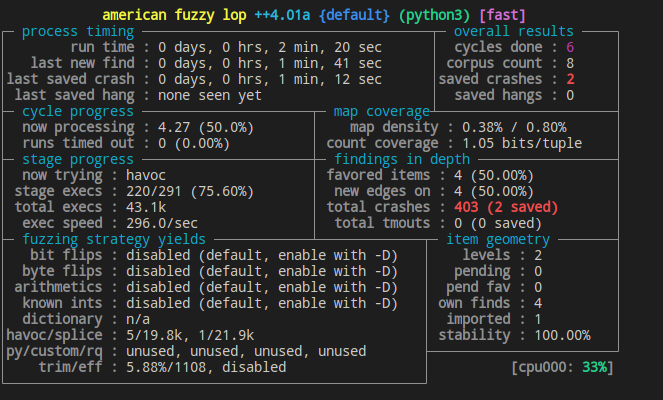
\includegraphics[scale=0.6]{QilingCheat.png}
    \caption{Fuzzing de UPNP con Qiling y AFL++ fijando manualmente el fin de la cadena mágica.}
    \label{fig:QilingCheat}
\end{figure}

\begin{figure}[H]
    \centering
    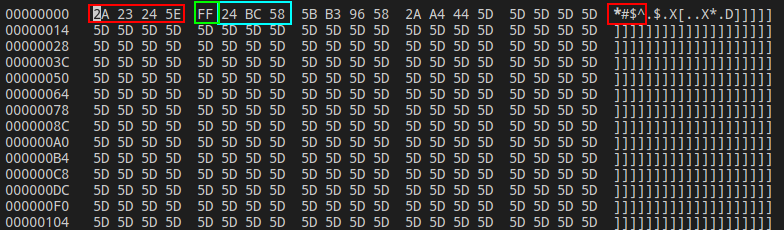
\includegraphics[scale=0.6]{UPNPQilingCrash.png}
    \caption{Cabecera firmware mutada por AFL++.}
    \label{fig:UPNPQilingCrash}
\end{figure}

Como hemos comentado, aunque la sesión de fuzzing no ha sido exitosa, Qiling ha dado muy buenos resultados a la hora de emular e instrumentar dinámicamente 
el binario. Es por ello que de estos resultados surge un pequeño experimento adicional. Esto es, integrar Radamsa con nuestro script de emulación de Qiling
para tener así un caso extra que nos permita comparar los resultados de fuzzear sobre emulación full-system en comparación con emulación basada en Unicorn 
manteniendo un mismo fuzzer. Respecto a las modificaciones del script, solo será necesario cambiar desde dónde obtiene el script el firmware por la misma
integración con Radamsa que hemos aplicado en el script de fuzzing a través de HTTP implementado anteriormente. Sorprendentemente, Radamsa
si que es capaz de identificar y respetar algunos de los campos presentes en las cabeceras, consiguiendo encontrar un crash en el binario
en aproximadamente 10 segundos haciendo uso del modo determinista y partiendo de la imagen firmware versión 1.0.11.134 (figura \ref{fig:UPNPQilingRadamsaCrash}).

\begin{figure}[H]
    \centering
    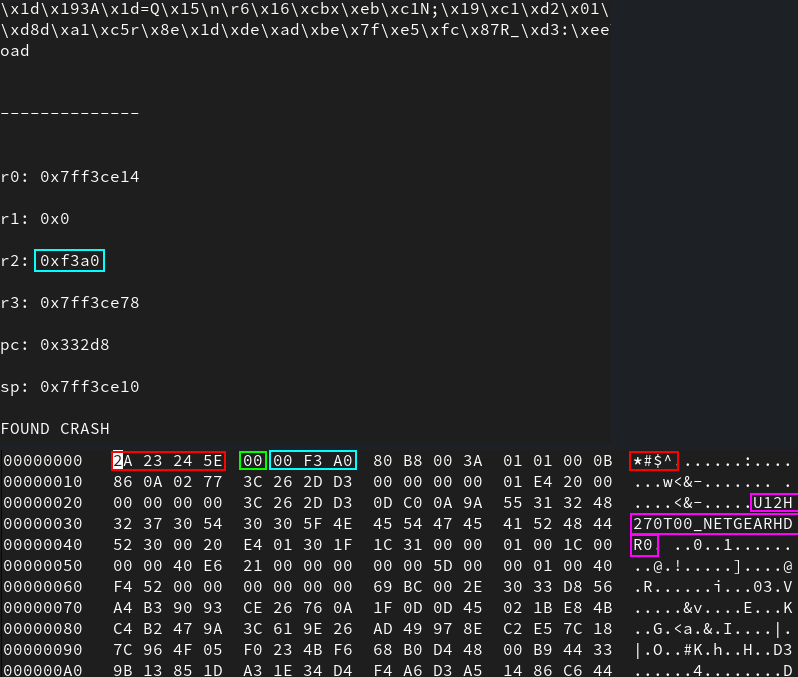
\includegraphics[scale=0.55]{UPNPQilingRadamsaCrash.png}
    \caption{Crash en UPNP identificado por Radamsa + Qiling.}
    \label{fig:UPNPQilingRadamsaCrash}
\end{figure}

\subsubsection{Fuzzing con QEMU full-system y Radamsa}
Al igual que Radamsa ha sido capaz de identificar el crash emulando el binario con Qiling en el caso anterior, también se ha llegado al mismo 
crash mediante el script desarrollado previamente que utiliza a Radamsa como fuzzer y va realizando peticiones SOAP a través de HTTP al 
demonio UPNP corriendo en la VM de QEMU ARM. La emulación tanto del sistema como del servicio ha sido estable durante todo el proceso de
fuzzing y UPNP era capaz de procesar correctamente las cabeceras del firmware enviado y de detectar si se producía algún fallo en la comprobación
de la cadena mágica o del checksum al igual que en Qiling. Para encontrar el mismo crash, partiendo de la misma semilla y funcionando en modo 
determinista, el script necesitó 1 minuto y 17 segundos (figura \ref{fig:UPNPQEMURadamsaCrash}), siendo el XML de la figura \ref{fig:UPNPQEMURadamsaCrashXML}
el causante del crash. Si comprobamos el estado del demonio en la VM (\ref{fig:UPNPsegfault}) observamos que como era de esperar, se ha producido un segmentation-fault
en la librería estándar de C (libc.so.0) mientras se realizaba la llamada a \textit{memcpy}.

\begin{figure}[H]
    \centering
    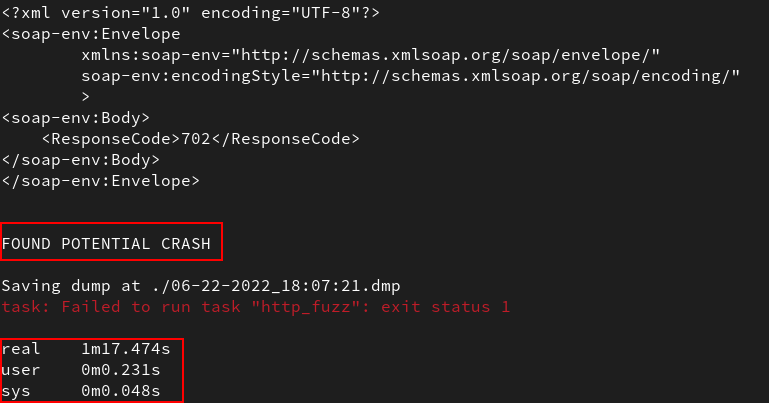
\includegraphics[scale=0.6]{UPNPQEMURadamsaCrash.png}
    \caption{Crash en UPNP identificado por Radamsa a través de peticiones HTTP.}
    \label{fig:UPNPQEMURadamsaCrash}
\end{figure}

\begin{figure}[H]
    \centering
    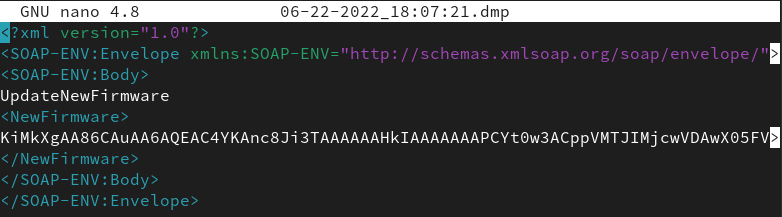
\includegraphics[scale=0.6]{UPNPQEMURadamsaCrashXML.png}
    \caption{Payload XML que ha causado el crash del servicio UPNP.}
    \label{fig:UPNPQEMURadamsaCrashXML}
\end{figure}

\begin{figure}[H]
    \centering
    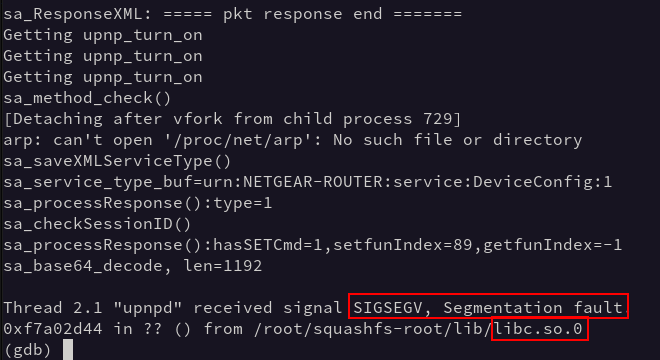
\includegraphics[scale=0.6]{UPNPsegfault.png}
    \caption{Segmentation-fault producido en UPNP durante el proceso de fuzzing HTTP.}
    \label{fig:UPNPsegfault}
\end{figure}

El gran incremento de tiempo para alcanzar la vulnerabilidad comparado con la aplicación de Radamsa junto a Qiling es comprensible, ya que 
no solo es necesario tener en cuenta el overhead de emular el sistema operativo al completo, sino que también las penalizaciones adicionales 
de rendimiento por emular el servicio al completo y por tener que enviar el firmware a través de peticiones HTTP.

\subsection{Lecciones aprendidas}
La realización de este experimento nos ha permitido sacar ciertas conclusiones respecto a la emulación y fuzzing de software orientado a IoT.
Principalmente podemos destacar los siguientes puntos:
\begin{itemize}
    \item Debido a que estamos ante una vulnerabilidad relativamente simple, hemos podido comprobar que hay casos para los que el uso de un 
    fuzzer de caja gris no aporta ninguna ventaja con respecto a aplicar fuzzing de caja negra. Obviando el bug de Unicornafl que hemos
    discutido, ambas técnicas han sido capaces de identificar la vulnerabilidad en periodos de tiempo similares.
    \item La integración de AFL++ con Unicorn/Qiling no está todavía lista para ser ampliamente adoptada por el público general. No es una 
    buena experiencia de usuario el no poder discernir si un problema encontrado durante el fuzzing es producido por un fallo personal 
    o por un fallo en la implementación de la herramienta.
    \item El uso del framework de Qiling resulta de gran utilidad cuando se quiere emular funcionalidad muy concreta de un binario y su 
    uso en combinación con otras herramientas de fuzzing facilita considerablemente el adaptar el binario al proceso de fuzzing gracias a 
    sus capacidades de instrumentación dinámica.
    \item Es recomendable depurar las sesiones de fuzzing para comprobar que el proceso se está realizando correctamente. En muchas ocasiones,
    es muy fácil cometer un error al realizar las preparaciones previas al fuzzing y es posible que aunque a primera vista el proceso se esté 
    llevando a cabo correctamente, realmente no se esté alcanzando el código que deseamos o no se estén identificando crashes que deberían de 
    ser registrados.
    \item La emulación full-system no nos permite prescindir completamente del hardware original, ya que como hemos podido comprobar, hay ciertos 
    casos para los que o se necesita extraer información del dispositivo original como variables de configuración o resulta difícil conseguir 
    emular a la perfección todos los periféricos requeridos.
\end{itemize}

\section{Análisis de un proyecto Open Source: Fuzzing de un parser JSON}
\subsection{Introducción al dispositivo}
La Wyzecam V3 (figura \ref{fig:wyzecam}) es una cámara de vigilancia WIFI de bajo coste fabricada por la empresa Wyze y lanzada al mercado
en 2020. Esta cámara representa
un claro ejemplo de dispositivo IoT, en el que toda la interacción con este se realiza a través de una aplicación móvil además de disponer de integración con 
tecnologías comúnmente encontradas en domótica como Google Assistant, Amazon Alexa e IFTT.

\begin{figure}[H]
    \centering
    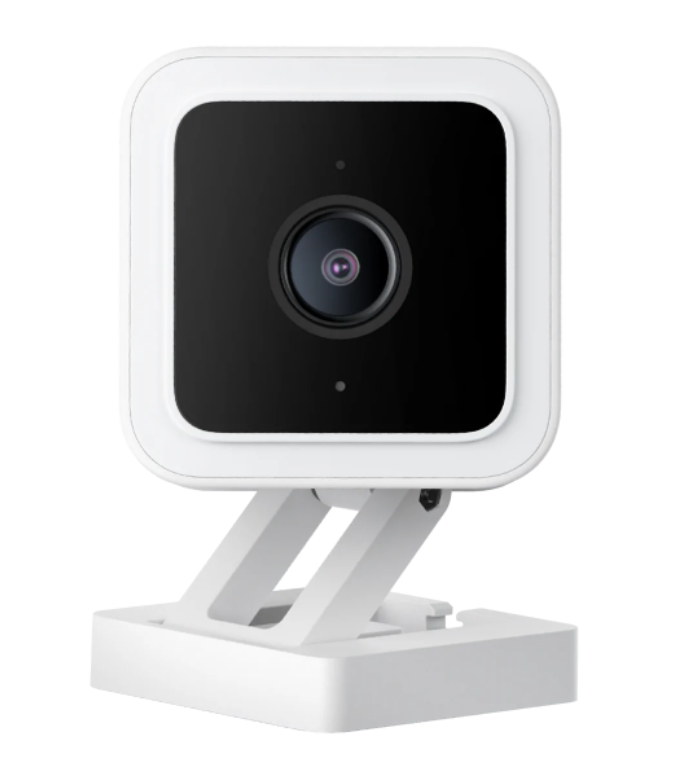
\includegraphics[scale=0.25]{wyzecam.png}
    \caption{Wyzecam V3.}
    \label{fig:wyzecam}
\end{figure}

\subsection{Recopilación de información}
Siguiendo el mismo procedimiento llevado a cabo en el apartado \ref{r7000_section} para obtener información más detallada sobre
el dispositivo, accedemos al reporte del FCC para la Wyzecam V3\cite{wyzecamFCCid} y a través de su listado de fotografías internas
identificamos su SoC. Rápidamente observamos que se trata de un ''Ingenic T31'' (figura \ref{fig:ingenict31}), un SoC orientado a procesamiento 
de vídeo. Consultando las especificaciones técnicas proporcionadas por el fabricante de este chip llegamos a un diagrama de bloques 
(figura \ref{fig:ingenicDiagram}) que nos indica que estamos ante un procesador modelo XBurst 1 con una arquitectura MIPS de 32 bits.
Para responder a la pregunta de si posee una MMU accedemos al manual de programación oficial del chip\cite{xburstmanual} y descubrimos 
que posee una MMU capaz de direccionar hasta 4GB de memoria.

\begin{figure}[H]
    \centering
    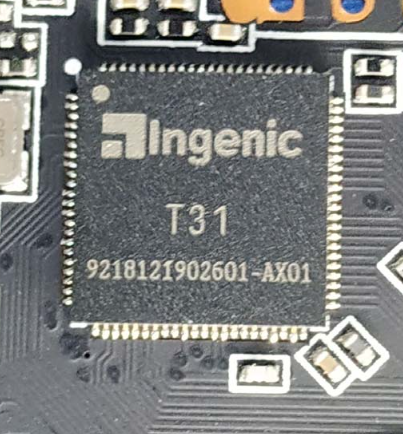
\includegraphics[scale=0.45]{ingenict31.png}
    \caption{SoC Ingenic T31 dentro de la Wyzecam V3\cite{wyzecamFCCid}.}
    \label{fig:ingenict31}
\end{figure}

\begin{figure}[H]
    \centering
    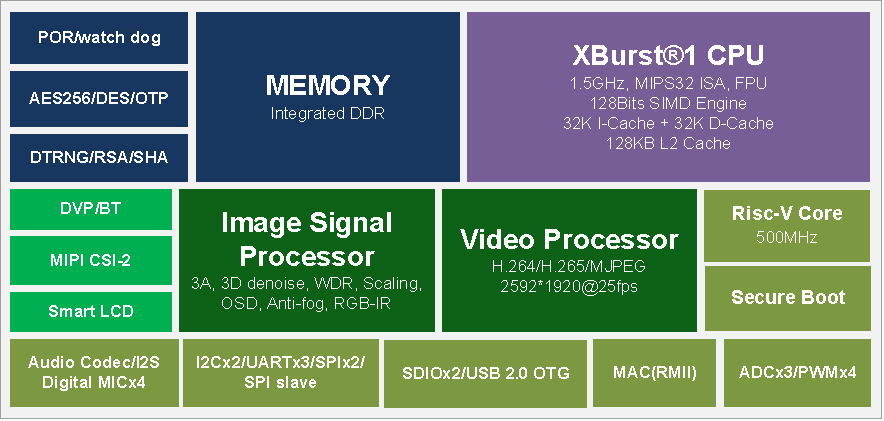
\includegraphics[scale=1.1]{ingenicDiagram.png}
    \caption{Diagrama de bloques del Ingenic T31\cite{ingenicproductpage}.}
    \label{fig:ingenicDiagram}
\end{figure}

\subsection{Obtención del firmware}
Para la obtención del firmware, accedemos al \href{https://support.wyze.com/hc/en-us/articles/360024852172-Release-Notes-Firmware}{portal de descargas}
de Wyze y descargamos la versión 4.36.8.26. El resultado es un fichero
con extensión ''.bin'' que procederemos a analizar con binwalk\cite{binwalk}. De la misma forma que anteriormente, empezamos consultando 
la entropía del firmware. Al hacerlo, como podemos observar en la figura \ref{fig:wyzeEntropy}, se muestra una entropía alta con caídas 
pronunciadas. Esto se debe a que el firmware está mayormente comprimido pero las cabeceras de sus secciones no lo están. Para comprobarlo,
utilizamos binwalk para obtener un reporte de los elementos contenidos dentro del binario y efectivamente, observamos que las caídas de 
la entropía dentro de los límites observables por binwalk se corresponden con la dirección de inicio de algunas de las secciones 
(figura \ref{fig:binwalkWyze}). También podemos ver que se utiliza un sistema de archivos SquashFS y que estamos ante un firmware basado
en Linux con un kernel versión 3.10.14 el cual fue publicado en 2013 y ha quedado ya considerablemente obsoleto. Por último, ya que se 
han detectado correctamente los contnidos del firmware, procedemos a su extracción para dar paso a la siguiente sección.

\begin{figure}[H]
    \centering
    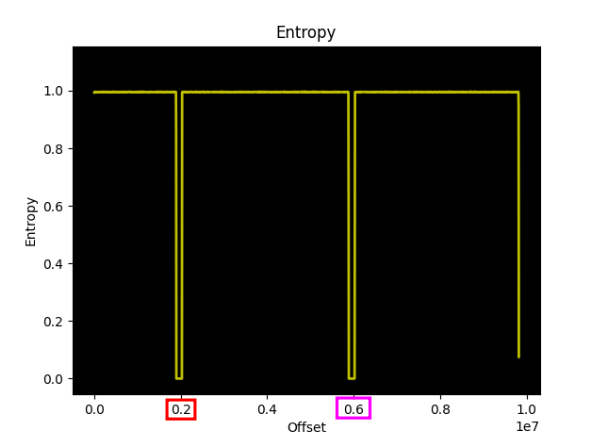
\includegraphics[scale=0.65]{wyzeEntropy.png}
    \caption{Entropía del firmware de la Wyzecam V3 versión 4.36.8.26.}
    \label{fig:wyzeEntropy}
\end{figure}

\begin{figure}[H]
    \centering
    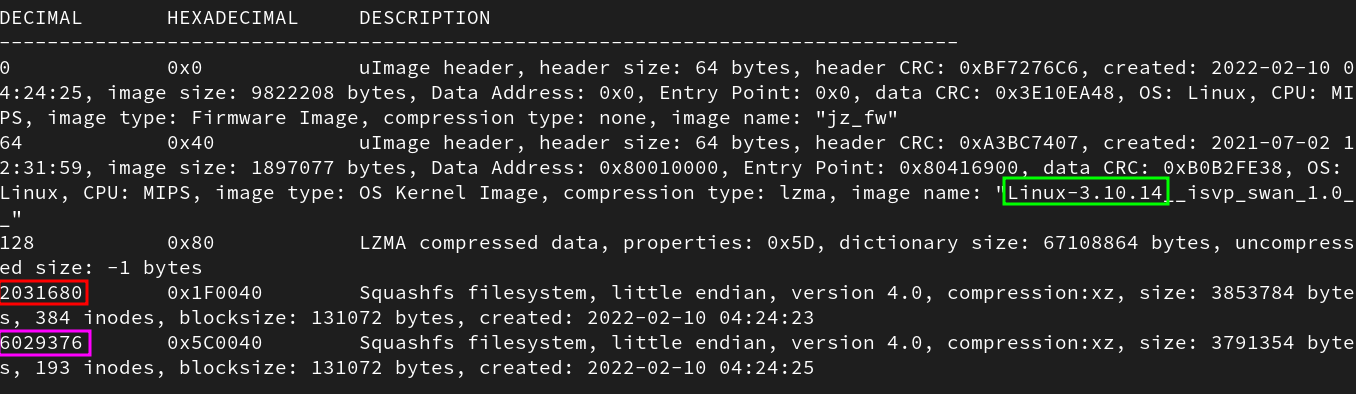
\includegraphics[scale=0.35]{binwalkWyze.png}
    \caption{Output de Binwalk sobre el firmware de la Wyzecam V3 versión 4.36.8.26.}
    \label{fig:binwalkWyze}
\end{figure}

\subsection{Introducción al experimento}
El componente software del firmware elegido para llevar a cabo este experimento es la librería cJSON\cite{cJSON}, un parser de JSON extremadamente 
ligero escrito en ANSI C. Dado su bajo impacto en los recursos del sistema, esta librería es comúnmente usada en sistemas empotrados para
ayudar con el tratamiento de información en formato JSON. La motivación principal detrás de elegir este software para aplicar fuzzing es
la siguiente:
\begin{itemize}
    \item \textbf{Distribuida como librería}: El hecho de que cJSON esté incluido en el firmware a modo de librería enlazada dinámicamente y no como un ejecutable
    como sucedía en el anterior experimento, implica la necesidad de tratar un nuevo aspecto del fuzzing, los harness.
    \item \textbf{Superficie de ataque}: Los dispositivos IoT se caracterizan entre otras cosas por tratar con órdenes y datos provenientes del exterior
    desde de otros dispositivos. Para comunicar de forma eficiente esta información se suelen utilizar formatos como JSON o XML y por tanto, se 
    requerirán parsers que traten con esos inputs externos. Un fallo en el tratamiento de estos datos puede dar lugar a comportamientos erráticos o 
    presentar una oportunidad para un atacante.
    \item \textbf{Open Source}: Teniendo en cuenta que nos estamos introduciendo por primera vez en el campo del reversing y fuzzing en este tipo de 
    dispositivos, tener acceso al código fuente original puede ayudarnos a analizar más fácilmente los crashes encontrados y sus causas. Además, 
    aunque teniendo acceso al código fuente podríamos simplemente recompilarlo para x86-64, el centrarnos en trabajar con la librería extraída del firmware 
    nos da la oportunidad de seguir expandiendo nuestros conocimientos sobre este campo pero con la ayuda adicional de poder consultar el código original.
\end{itemize}

Habiendo tratado con el experimento anterior el uso de Qiling en profundidad y dado que en esta ocasión tenemos control sobre el harness a utilizar, centraremos
este experimento en el fuzzing de caja gris a través de AFL++ en modo QEMU. Además, comprobaremos si es posible obtener una mejora de resultados mediante 
el uso de desinfectantes como QASAN en conjunción con el proceso de fuzzing. Por último, cabe destacar que en este caso no partimos buscando una vulnerabilidad
ya conocida, sino que nuestro objetivo es intentar descubrir nuevas vulnerabilidades en el producto.

\subsection{Realización del experimento}
\subsubsection{Creación del harness}
Como hemos comentado, debido a que estamos tratando con una librería enlazada dinámicamente por distintos componentes del firmware del dispositivo, necesitaremos
implementar código a modo de harness que se encargue de obtener los inputs como parámetro de la línea de comandos y llame a ciertas funciones de la librería.
Para decidir qué funciones de la librería poner a prueba, un buen criterio a seguir es tratar aquellas funciones que trabajen directamente 
con input externo. Para conocer el listado de funciones de que exporta la librería hay dos posibles rutas a seguir. En primer lugar, si tenemos acceso al código
fuente como es el caso, podemos simplemente incluir el header file de la librería en nuestro harness. En caso de no tenerlo, es posible listar las funciones
exportadas por una librería compartida con herramientas como ''objdump'' o ''nm'' (figura \ref{fig:objdump}) y definir en nuestro harness las funciones usando 
la keyword de C ''extern'' para indicar al
compilador que la función será resuelta en tiempo de enlazado. Además, querremos que las funciones elegidas sean utilizadas por el firmware del dispositivo, lo
cual podemos comprobar desde el sistema de archivos extraído del firmware haciendo uso de un ''grep'' recursivo para ver qué binarios importan la librería y usando la herramienta ''strings'' para listar
las funciones de cJSON utilizadas por el binario (en caso de que el binario no haya sido strippeado) (figura \ref{fig:cJSONimports}).

\begin{figure}[H]
    \centering
    \includegraphics[scale=0.5]{objdump.png}
    \caption{Listado de las funciones exportadas por la librería de cJSON.}
    \label{fig:objdump}
\end{figure}

\begin{figure}[H]
    \centering
    \includegraphics[scale=0.55]{cJSONimports.png}
    \caption{Listado de las funciones de la librería siendo utilizadas para un binario.}
    \label{fig:cJSONimports}
\end{figure}

Teniendo todo esto en cuenta, optamos por añadir al harness las siguientes funciones:
\begin{itemize}
    \item \textbf{cJSON\_Parse()}: Función principal encargada de parsear strings para generar una estructura de datos fácilmente manipulable que represente
    información en formato JSON. 
    \item \textbf{cJSON\_Minify()}: Función encargada de eliminar tokens innecesarios como saltos de línea de un input. Esta función va iterando sobre los
    caracteres de una string en busca de saltos de línea ($\backslash$n), retornos de carro ($\backslash$r) o tabulaciones ($\backslash$t), además de caracteres que 
    puedan indicar la presencia de comentarios de una o múltiples líneas con el fin de eliminar todo esto y generar una string solo con los datos en formato JSON.
    \item \textbf{cJSON\_Print()}: Función que imprime por pantalla el JSON parseado.
    \item \textbf{cJSON\_PrintBuffered()}: Alternativa a ''cJSON\_Print()'' que utiliza memoria dinámica.
\end{itemize}

Para la lectura de los inputs a partir de un fichero, implementamos la siguiente función que volcará el contenido del fichero en un array de bytes al que se le 
añadirá un byte nulo al final para indicar el fin del input y evitar así problemas con el tratamiento de los bytes en caso de que AFL++ genere una string mutada 
que no haya sido correctamente terminada.

\begin{lstlisting}[language=C, caption=Lectura de inputs desde fichero en el harness., captionpos=b,
    frame=single, breaklines, showstringspaces=false]
    char* read_input(char* path){
        FILE *f;
        struct stat st;
        char* content = NULL;
        size_t read_elements = 0;
    
        f = fopen(path, "rb");
        if (f == NULL)
            exit(1);
    
        stat(path, &st);
        if (st.st_size == 0)
            exit(1);
    
        content = (char*)malloc(st.st_size + 1);
        content[st.st_size] = '\0';                                                 // Avoid heap-buffer-overflow in strlen with non null terminated strings
        if (fread(content, st.st_size, 1, f) != 1 || strlen(content) == 0)
            exit(1);
        
        return content;
    }
\end{lstlisting}

Por último, compilamos el harness para MIPS indicándole al compilador que haga uso de la librería compartida de cJSON. Usaremos la 
siguiente orden con el compilador GCC de la toolchain de GNU para MIPS(el) y lo emulamos usando QEMU (figura \ref{fig:harnessRun}):

\begin{lstlisting}[language=bash]
    $ mipsel-linux-gnu-gcc -Iinclude src/harness.c -o bin/harness -lc -lcjson
\end{lstlisting}

\begin{figure}[H]
    \centering
    \includegraphics[scale=0.55]{harnessRun.png}
    \caption{Ejecución del harness en QEMU.}
    \label{fig:harnessRun}
\end{figure}

\subsubsection{Fuzzing de cJSON}
Comenzar la sesión de fuzzing con AFL++ en modo QEMU en sencillo, simplemente creamos un corpus de inputs 
con una serie de ficheros con datos en formato JSON e iniciamos AFL++ en modo QEMU (figura \ref{fig:harnessFuzz})
de la misma forma que se ha realizado en experimentos anteriores pero esta vez indicando con la variable de entorno
''AFL\_INST\_LIBS'' que deseamos que se instrumente también la ejecución de código en las librerías compartidas.

\begin{figure}[H]
    \centering
    \includegraphics[scale=0.5]{harnessFuzz.png}
    \caption{Fuzzing del harness con AFL++ en modo QEMU.}
    \label{fig:harnessFuzz}
\end{figure}

AFL++ permite activar el uso de desinfectantes en su modo QEMU utilizando la variable de entorno ''AFL\_USE\_QASAN''.
QASAN hará uso de las capacidades de instrumentación dinámica internas de QEMU para monitorizar operaciones de memoria 
en binarios que no han sido instrumentados estáticamente y forzar un crash en caso de detectar fallos de memoria. 
Sorprendentemente, al fijar esta variable de entorno AFL++ no era capaz de iniciar la sesión de fuzzing indicando que 
todas las ejecuciones realizadas con los inputs iniciales del corpus habían crasheado, como podemos 
observar en la figura \ref{fig:aflQASAN}

\begin{figure}[H]
    \centering
    \includegraphics[scale=0.5]{aflQASAN.png}
    \caption{Error mostrado por AFL++ al activar QASAN para fuzzear cJSON.}
    \label{fig:aflQASAN}
\end{figure}

\subsection{Resultados}
Durante la realización de este experimento, fue necesario hacer frente a una serie de problemas encontrados:
\begin{itemize}
    \item \textbf{Alto uso de I/O}: Cuando se realiza fuzzing, un factor que hemos de tener en cuenta es la carga 
    de I/O a la que el disco del host es sometido. En este experimento concretamente, el gran número de ejecuciones por 
    segundo y por tanto de escrituras de nuevos ficheros con inputs JSON mutados daba lugar a unos 7MB/s de escritura en 
    disco como podíamos comprobar con la herramienta ''iotop'' (figura \ref{fig:iotopBefore}). Mantener estas cifras de forma 
    prolongada durante horas puede suponer un desgaste considerable para el disco pero esto puede ser paliado haciendo uso 
    de un ramdisk. Un ramdisk consiste en asignar una sección de la RAM de un dispositivo para que actúe como si de un disco
    de almacenamiento se tratara. Para usar un ramdisk con AFL++ solo deberemos de crear un directorio en ''/dev/shm'' y usar la 
    variable de entorno ''AFL\_TMPDIR'' al iniciar la sesión de fuzzing para indicar que se desea utilizar el directorio creado para 
    la gestión de ficheros temporales durante el fuzzing. Este directorio especial se trata de un sistema de archivos temporal (tmpfs)
    encontrado en GNU/Linux que implementa el concepto de memoria compartida, utilizando RAM como medio de almacenamiento. Con este 
    cambio se consigue una reducción de escrituras en disco destacable, estando ahora ligeramente por encima de los 10KB/s 
    (figura \ref{fig:iotopAfter})
    \begin{figure}[H]
        \centering
        \includegraphics[scale=0.75]{iotopBefore.png}
        \caption{Uso de disco durante una sesión de fuzzing de cJSON.}
        \label{fig:iotopBefore}
    \end{figure}
    \begin{figure}[H]
        \centering
        \includegraphics[scale=0.54]{iotopAfter.png}
        \caption{Uso de disco tras utilizar un ramdisk durante una sesión de fuzzing de cJSON.}
        \label{fig:iotopAfter}
    \end{figure}
    \item \textbf{Aparición de falsos positivos}: Otro de los retos comúnmente encontrados durante el fuzzing es el poder diferenciar 
    cuando un crash detectado es un falso positivo y cuando se trata de un crash real, ya que pueden producirse falsos positivos por
    multitud de razones como fallos en el harness, fallos en la emulación o falta de memoria RAM en el host entre otros. Para hacer frente a esto, 
    un proceso de ''triaging'' es necesario. Este proceso consiste en un análisis más en profundidad de un crash detectado, en el que 
    el problema se intenta reproducir y posteriormente analizar con la ayuda de depuradores de código. De esta forma se descubre no solo 
    si el crash se produce realmente sino que también en qué punto del código lo está haciendo. Durante la sesión de fuzzing de nuestro 
    harness, se identificó que los crashes que estaban siendo detectados eran falsos positivos producidos en la lógica de lectura de 
    ficheros del harness y no en el código de la librería. Esto se debía a que en el harness se realizaban llamadas a funciones de 
    tratamiento de strings como \textit{strlen}, las cuales dependen de que la cadena esté adecuadamente terminada con un byte nulo y 
    como es de esperar, AFL++ realizaba ciertas mutaciones que carecían de dicho byte al final de la cadena JSON. Para solucionar esto,
    añadiremos manualmente un byte nulo al final de la cadena mutada antes de pasarla a las funciones de cJSON. 
    \item \textbf{Problemas para utilizar QASAN}: En un principio se desconocía el motivo por el cual AFL++ no era capaz de iniciar el 
    fuzzing al activar QASAN. Sabiendo que todas las ejecuciones iniciales con los inputs del corpus han crasheado pero sin saber el 
    por qué, iniciamos de nuevo un proceso de triaging en el que buscamos identificar qué origina los crashes. El primer paso es mostrar 
    el output de cada una de las ejecuciones preliminares que realiza AFL++ con la variable de entorno ''AFL\_DEBUG\_CHILD''. Tras hacer esto,
    observamos que en todas las ejecuciones QASAN detecta un heap-buffer-overflow en el código de la librería, concretamente en \textit{libcjson.so.1+0x8dc0}
    (figura \ref{fig:QASANfuzz}). Esto nos indica que estamos ante un fallo de memoria producido en cJSON que aunque en circunstancias normales
    no afecta al correcto funcionamiento del código, QASAN fuerza un crash al detectarlo. Trataremos más en profundidad este fallo a continuación.
    \begin{figure}[H]
        \centering
        \includegraphics[scale=0.42]{QASANfuzz.png}
        \caption{Resultado de la emulación del harness con QASAN activado.}
        \label{fig:QASANfuzz}
    \end{figure}
\end{itemize}
Una vez fue solucionado el problema comentado con el harness, en la sesión de fuzzing empezaron a aparecer crashes que ahora sí que sucedían dentro 
del código de la librería de cJSON. Tras tres horas de fuzzing sin QASAN, se procedió a intentar obtener más información sobre los crashes identificados con la 
sorpresa de que al intentar ejecutar el harness con los inputs problemáticos el crash no era reproducible. Dado que es posible usar QASAN para 
ejecuciones individuales fuera del fuzzing, lo utilizamos para obtener más información sobre los supuestos crashes y descubrimos que aunque el
crash en sí no puede ser reproducido, QASAN es capaz de indicarnos que se han producido tres heap-buffer-overflows en distintas funciones del código 
de cJSON.
\begin{itemize}
    \item \textbf{cJSON\_Minify()}: El reporte mostrado por QASAN (figura \ref{fig:cJSONminify}) nos indica que se ha producido un acceso 0 bytes más allá de los límites de un espacio
    de memoria reservado en el heap de 29 bytes. Podemos apreciar fácilmente lo sucedido en el mapa de ''shadow-bytes'' mostrado por QASAN, donde se 
    almacenan metadatos sobre el mapa de memoria principal. Teniendo en cuenta que cada byte mostrado en el mapa de shadow-bytes representa 8 bytes 
    de memoria principal de la aplicación y que ''00'' indica que los 8 bytes son direccionables, observamos como hay reservados 29 bytes ($3\cdot8 + 5=29$)
    siendo el acceso fuera de límites en el tramo entre los últimos ( 5 - 8 ] bytes, concretamente en el byte inmediato siguiente a los límites 
    direccionables. Si consultamos en Ghidra el código ubicado en \textit{libcjson.so.1+0x8e8c} y lo comparamos con el código fuente original, descubrimos
    que la operación se da al leer un byte más allá de la cadena de caracteres recibida como parámetro de la función (figura \ref{fig:cJSONminifySource}).
    \begin{figure}[H]
        \centering
        \includegraphics[scale=0.32]{cJSONminify.png}
        \caption{Reporte del fallo de memoria en cJSON generado por QASAN.}
        \label{fig:cJSONminify}
    \end{figure}

    \begin{figure}[H]
        \centering
        \includegraphics[scale=0.45]{cJSONminifySource.png}
        \caption{Segmento de código donde se produce el heap-buffer-overflow.}
        \label{fig:cJSONminifySource}
    \end{figure}

    \item \textbf{skip\_multiline\_comment()}: Se trata de una función utilizada por \textit{cJSON\_Minify()} encargada de eliminar de una cadena de texto
    los comentarios en formato ''/* \dots */''. Analizando el reporte de QASAN vemos en el mapa de shadow-bytes (figura \ref{fig:QASANskipMultiline}) que de nuevo,
    se ha producido un acceso al byte inmediato siguiente de la sección de memoria reservada en \textit{libcjson.so.1+0x8b78}. Si navegamos en Ghidra a la 
    dirección especificada vemos que la operación es un incremento de un puntero en una posición (figura \ref{fig:GhidraSkipMultiline}). Si consultamos el 
    código original (figura \ref{fig:SkipMultilineSource}), confirmamos que simplemente se trata de un bucle for que se excede en una iteración al operar con una string.

    \begin{figure}[H]
        \centering
        \includegraphics[scale=0.55]{QASANskipMultiline.png}
        \caption{Mapa de shadow-bytes reportado por QASAN para la función \textit{skip\_multiline\_comment()}.}
        \label{fig:QASANskipMultiline}
    \end{figure}

    \begin{figure}[H]
        \centering
        \includegraphics[scale=0.6]{GhidraSkipMultiline.png}
        \caption{Decompilado de la función \textit{skip\_multiline\_comment()} en Ghidra.}
        \label{fig:GhidraSkipMultiline}
    \end{figure}

    \begin{figure}[H]
        \centering
        \includegraphics[scale=0.46]{SkipMultilineSource.png}
        \caption{Código fuente original de la función \textit{skip\_multiline\_comment()}.}
        \label{fig:SkipMultilineSource}
    \end{figure}
\end{itemize}

Como conclusión, comentar que ambos fallos no son de gran relevancia y que no suponen una amenaza real para el software que haga uso de esta librería.
Aún así, la metodología seguida para su análisis es igual de válida para vulnerabilidades más severas y gracias a su aplicación, se ha podido 
llevar a cabo un valioso caso práctico de uso de fuzzing en combinación con desinfectantes para la identificación de vulnerabilidades en software orientado 
a IoT.
\subsection{Lecciones aprendidas}
Siendo este el experimento que concluye el proyecto, finalizamos esta sección comentando las lecciones que hemos obtenido durante su realización. El haber
tenido la oportunidad de utilizar desinfectantes y la necesidad de crear nuestro propio harness nos han servido para expandir nuestros conocimientos más allá
de lo aprendido en el experimento anterior. Destacamos los siguientes puntos:
\begin{itemize}
    \item Aunque el usar desinfectantes durante el fuzzing puede hacer que se muestren fallos de memoria irrelevantes desde el punto de vista de la búsqueda 
    de vulnerabilidades, se ha demostrado que no solo ayudan de forma efectiva a los fuzzers en su tarea reduciendo el tiempo que necesitan para llegar a un 
    crash sino que también facilitan considerablemente el proceso de análisis de estos, proporcionando información muy valiosa al respecto como el mapa de 
    shadow-bytes.
    \item Hemos aprendido que no todos los fallos de memoria llevan a un crash completo de la aplicación. Algunos como los que hemos tratado en este experimento
    resultan inofensivos mientras que otros simplemente provocan un comportamiento indefinido sin interrumpir su ejecución.
    \item Es necesario prestar especial atención durante la creación de los harness ya que su utilización implica añadir código adicional que también puede
    originar fallos, dificultando así la tarea de discernir qué fallos realmente son producidos por el código que deseamos poner a prueba.
    \item Por último, se ha demostrado como en algunos casos es recomendable el uso de un ramdisk durante el fuzzing para evitar acelerar el desgaste del
    disco del sistema en el que esté siendo realizado, aún más cuando se planea llevar a cabo sesiones de fuzzing de larga duración.
\end{itemize}

	% Conclusiones
	\chapter{Conclusiones y trabajos futuros}
\label{conclusiones}
	
	\newpage
	\bibliography{bibliografia}
	\bibliographystyle{plain}
	
\end{document}

